\section{\texorpdfstring{The $\Wln$  Signal Extraction}{The W-> l nu  Signal Extraction}}
\label{sec:WsignalExtraction}

The signal and background yields are obtained by fitting
the $\MET$ distributions for $\Wen$ and $\Wmn$ to different
functional models.
An accurate $\MET$ measurement is essential for distinguishing
a $\PW$ signal from QCD multijet backgrounds.
We profit from the application of the PF
algorithm, which provides superior $\MET$
reconstruction performance~\cite{PFMET1} with respect to alternative
algorithms at the energy scale of the $\PW$ boson.
% The energy of photons is directly obtained from the ECAL measurement,
% corrected for zero-suppression effects.
% The energy of electrons is determined from a combination of the track
% momentum at
% the main interaction vertex, the corresponding ECAL cluster energy,
% and the energy sum of
% all bremsstrahlung photons attached to the track. The energy of muons
% is obtained from the
% corresponding track momentum. The energy of charged hadrons is
% determined from a combination
% of the track momentum and the corresponding ECAL and HCAL energy,
% corrected for
% zero-suppression effects, and calibrated for the non-linear response
% of the calorimeters. Finally
% the energy of neutral hadrons is obtained from the corresponding
% calibrated ECAL and HCAL
% energy.


The $\MET$ is the magnitude of the transverse component of the missing momentum
vector, computed as the negative of the vector sum of all
reconstructed transverse momenta of particles identified with
the PF algorithm. The algorithm combines the information from
the inner tracker, the muon chambers, and the calorimeters
to classify reconstructed objects according to particle type
(electron, muon, photon, or charged or neutral hadron),
thereby allowing precise energy corrections.
The use of the tracker information reduces the sensitivity of $\MET$ to miscalibration of the calorimetry.
%also providing a significant degree of redundancy that
%reduces the sensitivity of the $\MET$ measurements
%to miscalibrations of the calorimetry.
%\par
%The impact of anomalous noise signal in the calorimeters is reduced to
%a negligible level~\cite{metPAS}.

\par
The QCD multijet background is one of the most significant backgrounds in W analyses.
At high $\MET$, EWK backgrounds, in particular $\Wtn$ and DY,
also become relevant, leading to contamination levels on the
order of $10\%$.

The $\MET$ model is fitted to the observed distribution as the sum of three contributions:
the W signal, and the QCD and EWK backgrounds.
The EWK contributions are normalized to the W signal yield in the fit
through the ratios of the theoretical cross sections.

Simultaneous fits are performed to the two $\MET$ spectra of W$^+$ and W$^-$ candidates,
fitting either the total W cross section and
the ratio of positive and negative W cross sections, or
the individual positive and negative W cross sections.
In both cases the overall normalization of QCD multijet events is determined from the fit.
The diboson and $\ttbar$ contributions,
taken from simulations, are negligible (Section~\ref{sec:EWKbkgds}).


\par
In the following sections the modeling
of the $\MET$ shape for the signal and the EWK backgrounds are presented,
and the methods used to determine
the $\MET$ shape for the QCD multijet background from data are
 described.
Finally, the extraction of the signal yields is discussed.



%\section{Missing Transverse Energy\label{sec:MET}}
An accurate $\MET$ measurement is essential for distinguishing
$\Wo$ signal from QCD backgrounds. We use $\MET$ estimate provided
by the Particle Flow (PF) algorithm which showed the best performance for the
CMS detector. Details on Particle Flow $\MET$ are provided in Ref.~\cite{PFMET}. 
\par
We have very good agreement of the $\MET$
distributions in $\Wln$ in data and simulation~\cite{metPAS}.
\par
The $\MET$ is computed as the vector sum of all PF objects.
The resolution for inclusive multi-jet samples and for
$\Wln$ events is well reproduced by the 
simulation.  A modest broadening of about $10\%$ is observed 
when there is more than one primary vertex; this occurs in less 
than $40\%$ of the events and has a negligible impact on the
extraction of the $W$ yields described below.



\subsection{\texorpdfstring{Signal ${E\!\!/}_{\!\mathrm{T}}$  Modeling}{Signal ET Modeling}}
\label{sec:WsignalMETtemplate}

The $\Wln$ signal is extracted with methods that employ
simulation predictions of the $\MET$ distribution in signal events.
These predictions
rely on the modeling of the vector-boson recoil and detector effects that
can be difficult to simulate accurately. Discrepancies could result
from deficiencies in the modeling of the
calorimeter response and resolution, and from an incomplete description of
the underlying event.
% and from simplifications made in the simulation of pile-up.
These residual effects are addressed using corrections
determined from the study of Z-boson recoil in data, discussed in the following paragraph.

The recoil to the vector boson is defined as the negative of the vector
sum of transverse energy vectors of all particles reconstructed with the PF algorithm
in W and Z events, after subtracting the contribution from the daughter lepton(s).
The recoil is determined for each event in $\Zll$ data and simulated $\Zll$
and $\Wln$ samples.
We fit the distributions of the recoil components (parallel and perpendicular to the
boson p$_T$ direction) with a double Gaussian, whose mean and width vary with the boson
transverse momentum.
For each sample, we fit polynomials to the extracted mean and width of the recoil
distributions as functions of the boson transverse momentum.
The ratios of data to simulation fit-parameters from the $\Zo$ samples are used as scale
factors to correct the polynomials parameters of the W simulated recoil curves.
For each $\Wo$ simulated event, the recoil is replaced with a value drawn from the
distribution obtained with the corrected parameters corresponding to the $\Wo$ p$_T$.
The $\MET$ value is calculated by adding back the energy of the $\Wo$ lepton.
%We fit the recoil distributions whose mean and width vary with the boson transverse
%momentum. For each sample, we fit polynomials to the extracted means and widths of the recoil
%distributions as functions of the boson transverse momentum.
%The ratios of data to simulation fit parameters from the $\Zo$ samples are used as
%scale factors to correct the simulated $\Wo$ recoil curves. The recoil in simulated $\Wo$ events
%is replaced with the values drawn from the corrected W recoil distributions,
%adding the energy of the W leptons back to recalculate the $\MET$ value for each event.
The energy of the lepton used in the
calculation is corrected for the energy-scale and resolution effects.  Statistical
uncertainties from the fits are propagated into the $\MET$ distribution as systematic
uncertainties.  An additional systematic uncertainty is included to account for possible
differences in the recoil behavior of the W and Z bosons.

The same strategy is followed for the recoil corrections in the electron and muon analyses.
As an example, Fig.~\ref{fig:Recoil} (left) shows the effect of the recoil
corrections on the $\MET$ shape for simulated events in the electron channel, while Fig.~\ref{fig:Recoil} (right)
shows the uncertainty from the recoil method propagated to the corrected $\MET$ shape
of $\Wen$ events. The distribution of the residuals, $\chi$, is shown at the bottom of each plot,
where $\chi$ is defined as the per-bin difference of the two distributions, divided by the
corresponding statistical uncertainty. The same definition is used throughout this paper.

The systematic uncertainties on the signal $\MET$ shape are propagated as systematic
uncertainties on the extracted signal yield through the fitting procedure.
Signal shapes are determined for the W$^+$ and W$^-$ separately.

%%%%%%%%%%%%%%%%%%%%%%%%%
\begin{figure}
\begin{center}
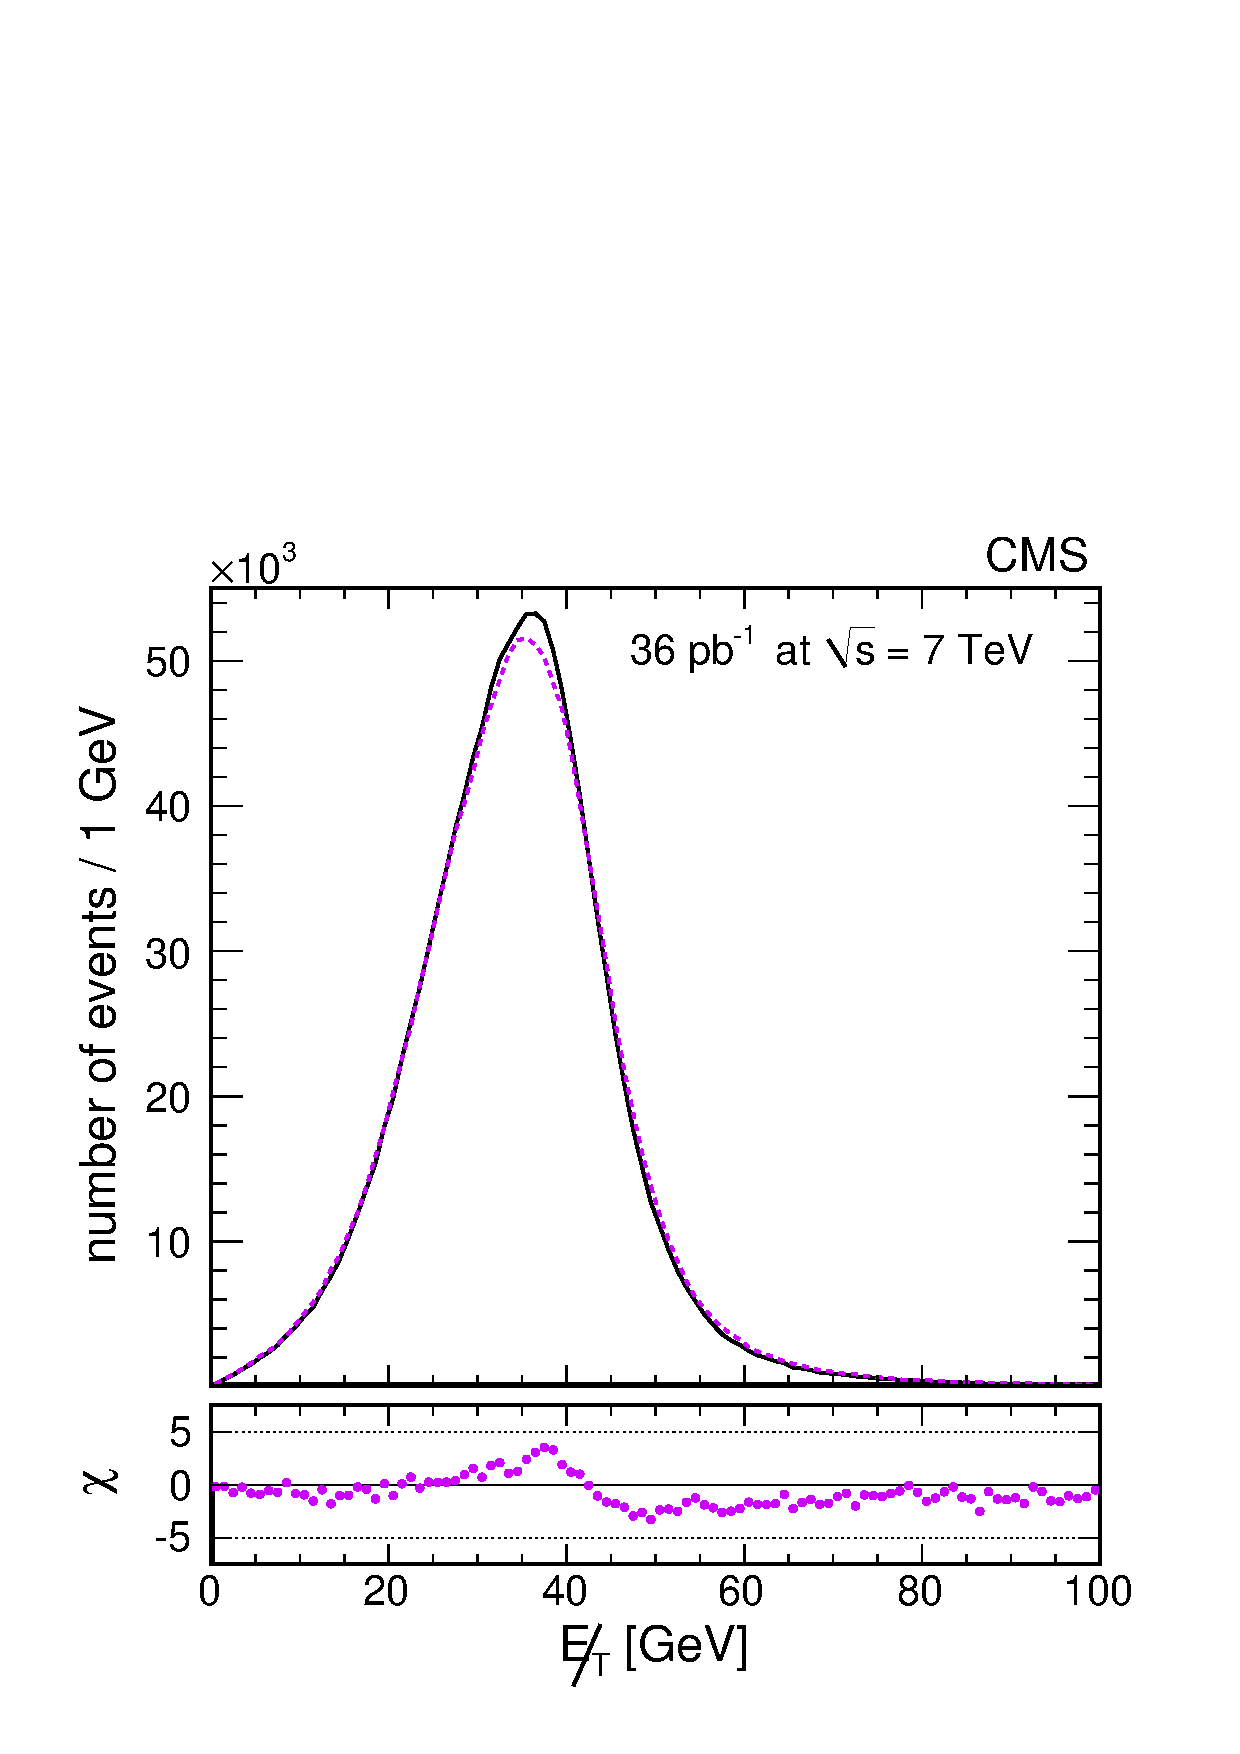
\includegraphics[width=0.48\textwidth]{figs/beforeANDafter.pdf}
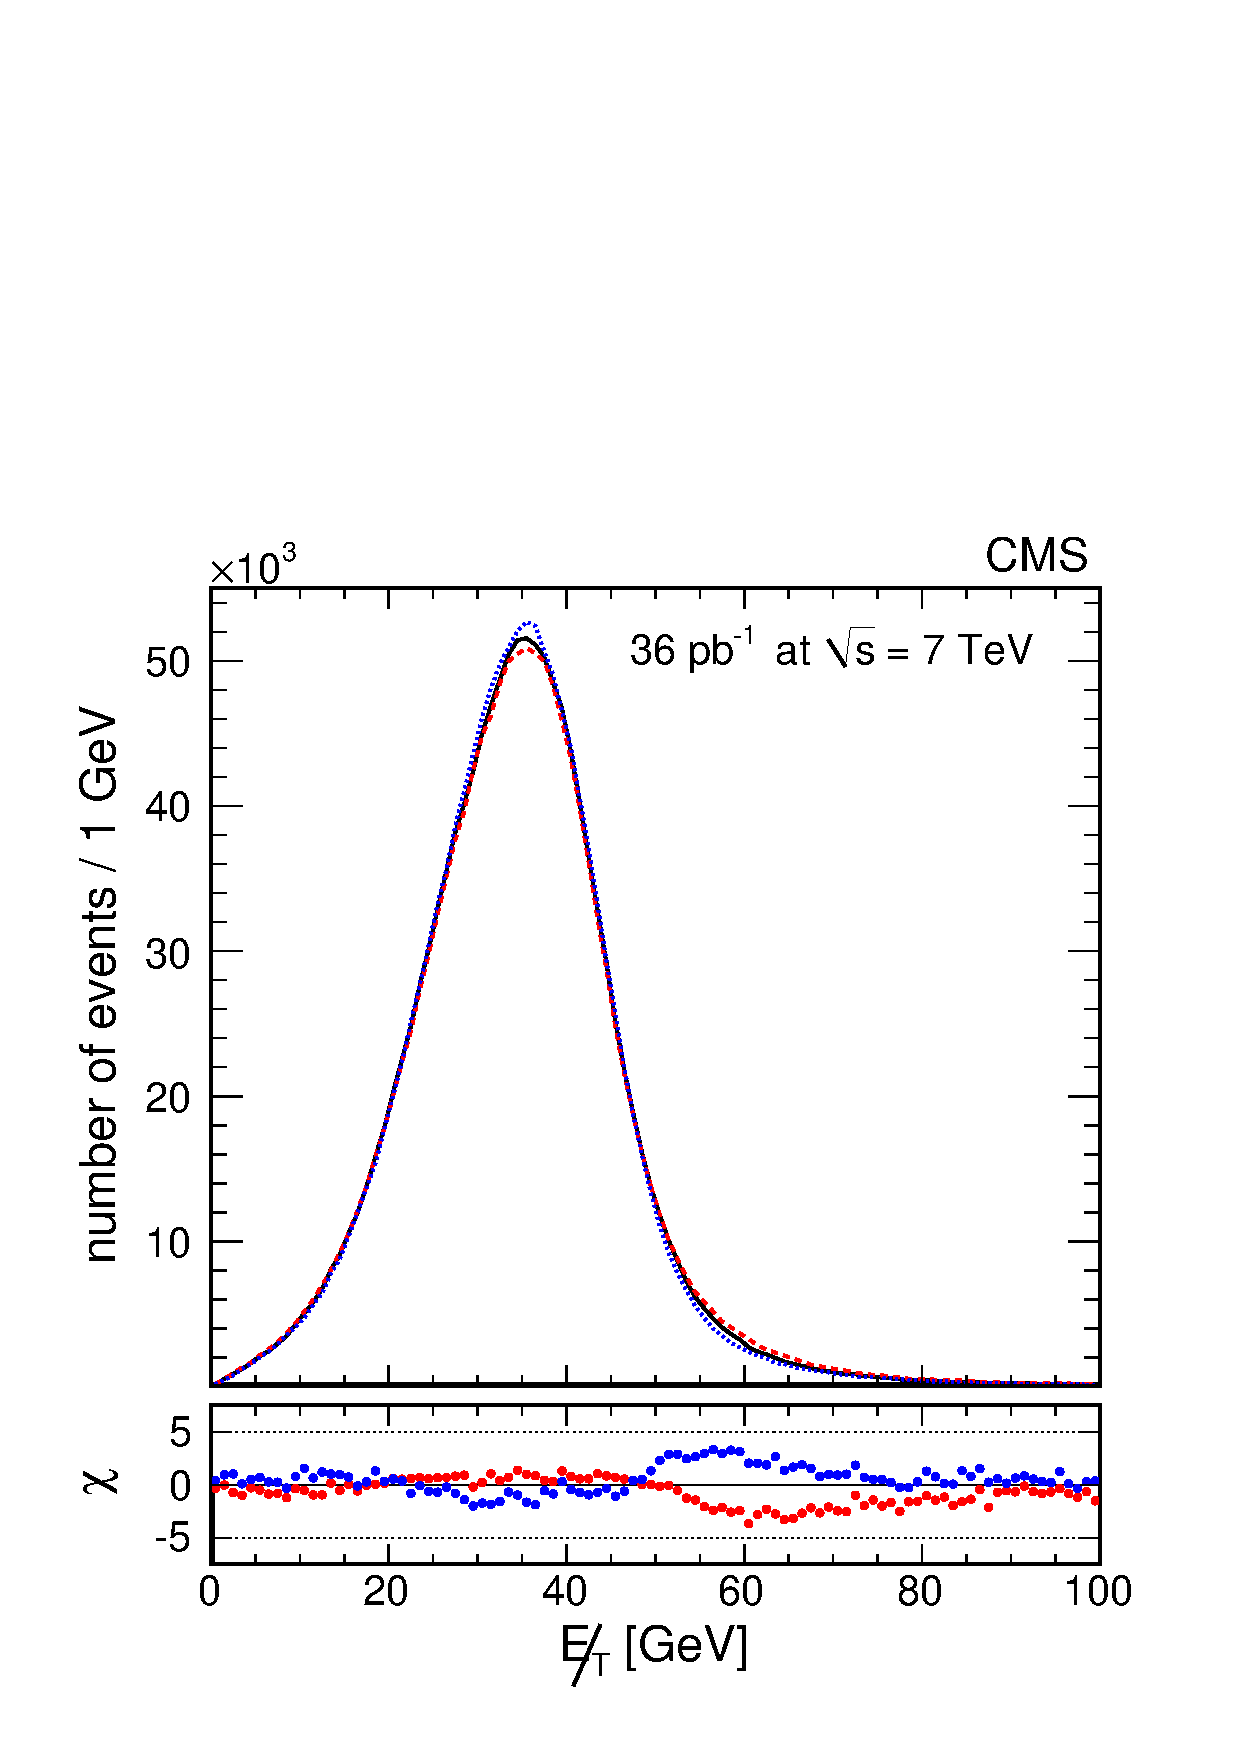
\includegraphics[width=0.48\textwidth]{figs/upANDdown.pdf}
\caption{ \label{fig:Recoil}
Left: simulated $\MET$ distribution in $\Wen$ events before (continuous black line)
and after (dashed red line) recoil corrections.
Right: the uncertainties from the recoil method propagated
to the corrected $\MET$ shape of $\Wen$ events (continuous black line, identical to the dashed
red line on the left-hand side plot) are presented with the red-dashed and blue-dotted lines.
These two shapes are obtained when the recoil systematic uncertainties are varied
by one standard deviation.
At the bottom of each plot is shown the distribution of the residuals, $\chi$, defined
as the per-bin difference of the two distributions, divided by the
corresponding statistical uncertainty.
}
\end{center}
\end{figure}
%%%%%%%%%%%%%%%%%%%%%%%%%


\subsection{Electroweak Backgrounds}
\label{sec:EWKbkgds}

A certain fraction of the events passing the selection criteria for $\Wln$
are due to other EWK processes. Several sources of
contamination have been identified. The events with $\Zll$ 
(DY background), where one of the two leptons lies
beyond the detector acceptance and escapes
detection, mimic the signature of $\Wln$ events. Events from $\Ztt$ and $\Wtn$,
with the tau decaying leptonically, have in general a lower-momentum lepton than signal
events and are strongly suppressed by the minimum $\Pt$ requirements.

The $\MET$ shape for the EWK vector boson and ${\mathrm t}\bar{\mathrm t}$ contributions are
evaluated from simulations. For the main EWK backgrounds ($\Zll$ and $\Wtn $), the $\MET$ shape is 
corrected by means of the procedure described in Section~\ref{sec:WsignalMETtemplate}.
The $\MET$ shapes are evaluated separately for $\Wptn$ and $\Wmtn$.

A summary of the background fractions in the $\Wen$ and $\Wmn$ analyses can be found in Table~\ref{tab:WlnBG}.
The fractions are similar for the $\Wen$ and $\Wmn$ channels, 
except for the DY background which is higher in the $\Wen$ channel. 
The difference is mainly due to the tighter definition of the DY veto in the $\Wmn$ channel, 
which is not compensated by the larger geometrical acceptance of electrons 
($|\eta|<2.5$) with respect to muons ($|\eta|<2.1$).
% with respect to $\Wen$ channel (the electron analysis rejects an event 
%if there is a second electron with $\Et>20.0\GeV$ while the muon analysis 
%rejects an event if there is a second muon with $\Pt>10\GeV$).

\begin{table} %
\begin{center}
\caption{\label{tab:WlnBG}
Estimated background-to-signal ratios in the $\Wen$ and $\Wmn$ channels.}

\begin{tabular}{|l|c|c|}
\hline
{\multirow{2}{*}{Processes}} & \multicolumn{2}{c|}{Bkg. to sig. ratio}  \\ \cline{2-3}
                           & $\Wen$ & $\Wmn$ \\ 
\hline \hline
$\Zee,\, \mu^+\mu^-,\, \tau^+\tau^-$ (DY)               & 7.6\%  &  4.6\% \\
$\Wtn $                    & 3.0\%  & $3.0$\%    \\
$\Wo\Wo$+$\Wo\Zo$+$\Zo\Zo$ & 0.1\% & $0.1$\%   \\
$\ttbar$                   & 0.4\% & $0.4$\%   \\
\hline
Total EWK                  & 11.2\%& $8.1$\% \\
\hline
\end{tabular}
\end{center}
\end{table}

%In the fit procedure described in the following Section, the relative normalization of the 
%EWK backgrounds is kept fixed to the values shown in Table~\ref{tab:WlnBG}.

% \begin{table}
% \begin{center}
% \begin{tabular}{|l|c|c|}
% \hline
% source & $\Nbg/(N_\Wo+\Nbg)$ & $\Nbg$ in $36.$~pb$^{-1}$ \\
% \hline\hline
% QCD multi-jet            & $5.1$\% & 8896  \\
% \hline
% $\Wtn$                   & $2.7$\%  &  4667  \\
% $\Ztt$                   & $0.5$\%  &   911  \\
% $\Wo\Wo$+$\Wo\Zo$+$\Zo\Zo$           & $0.1$\%  &   205  \\
% $\ttbar$                 & $0.3$\%  &   592  \\
% \hline
% EWK + $\ttbar$           & $7.1$\%  &  12538 \\
% \hline
% total                    & $12.2$\% &  21434 \\
% \hline
% $\Wmn$ signal            & $87.8$\%  & 153940 \\
% \hline
% \end{tabular}
% \caption{Estimates of backgrounds in the $\Wmn$ channel, based on Monte Carlo simulations.}
% \label{table:WmnBG}
% \end{center}
% \end{table}






\subsection{\texorpdfstring{Modeling of the QCD Background and $\Wen$ Signal Yield}{Modeling of the QCD Background and W-> e nu Signal Yield}}
\label{sec:WQCDbkg}

Three signal extraction methods are used, which give consistent
signal yields. The method described in Section~\ref{sec:AnalyticalFunction}
is used to extract the final result.

\subsubsection{Modeling the QCD Background Shape with an Analytical Function}
\label{sec:AnalyticalFunction}

The $\Wen$ signal is extracted using an unbinned maximum likelihood
(UML) fit to the $\MET$ distribution.
%Signal and EWK background
%distributions are derived from simulation and are validated using dedicated studies.

The shape of the $\MET$ distribution for the QCD background is modeled by a parametric function (modified Rayleigh
distribution) whose expression is
\begin{equation}
f_{\mathrm{CQD}}(\MET) = \MET\exp\left(-\frac{\MET{^2}}{2(\sigma_0+\sigma_1 \MET)^{2}}\right)\,.
\label{eq:rayleigh}
\end{equation}
The fit to a control sample, defined by inverting the track-cluster matching selection
variables $\Delta\eta$, $\Delta\phi$, shown in Fig.~\ref{fig:e-inverted}, illustrates
the quality of the description of the background shape by the parameterized function,
including the region of the signal, at high \MET.
\begin{figure}[htbp]
\begin{center}
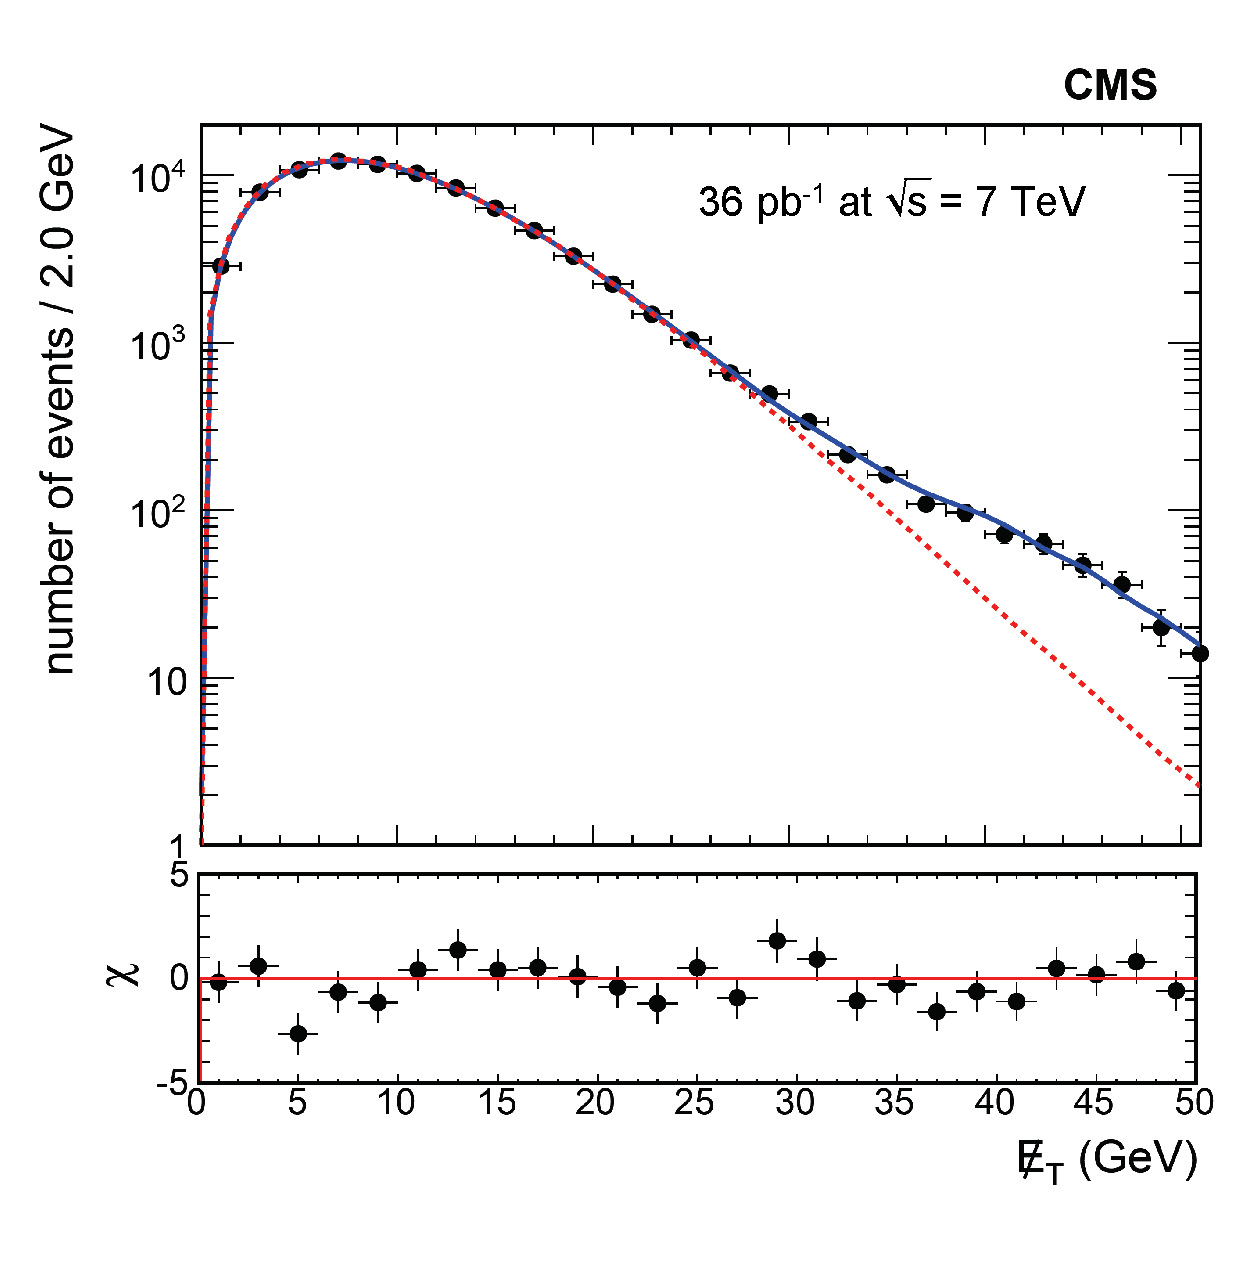
\includegraphics[width=0.50\textwidth]{figs/fixedMCyield_normal_model.pdf}
\caption{Fit to the background-dominated control sample defined by inverting
the selection on the track-match variables,
while maintaining the rest of the signal selection.
The blue solid line represents the model used to fit the control data sample. This is a Rayleigh
function plus a floating-yield signal shape that accounts for the signal contamination in the
control region. The magenta dashed line shows the Rayleigh function alone with its parameters estimated
from the combined fit.
}\label{fig:e-inverted}
\end{center}
\end{figure}
To study the systematic uncertainties associated with the background shape, the resolution term in
Eq.~(\ref{eq:rayleigh}) was changed by introducing an additional QCD shape parameter $\sigma_2$,
thus: $\sigma_0 + \sigma_1 \MET + \sigma_2 \MET^2$.

The free parameters of the UML fit are the QCD background yield,
the $\Wo$ signal yield, and the background shape
parameters $\sigma_0$ and $\sigma_1$.
The following signal yields are obtained:
$\WEIYIELD$ for the inclusive sample, $\WEPYIELD$ for the $\Wpen$ sample, and
$\WEMYIELD$ for the $\Wmen$ sample.
%with negligible correlation between the $\Wp$ and $\Wm$ yields.
The fit to the inclusive $\Wen$ sample is displayed
in Fig.~\ref{fig:Wen}, while the fits for the charge-specific
channels are displayed in Fig.~\ref{fig:WenPM}.

\begin{figure}[htbp]
\begin{center}
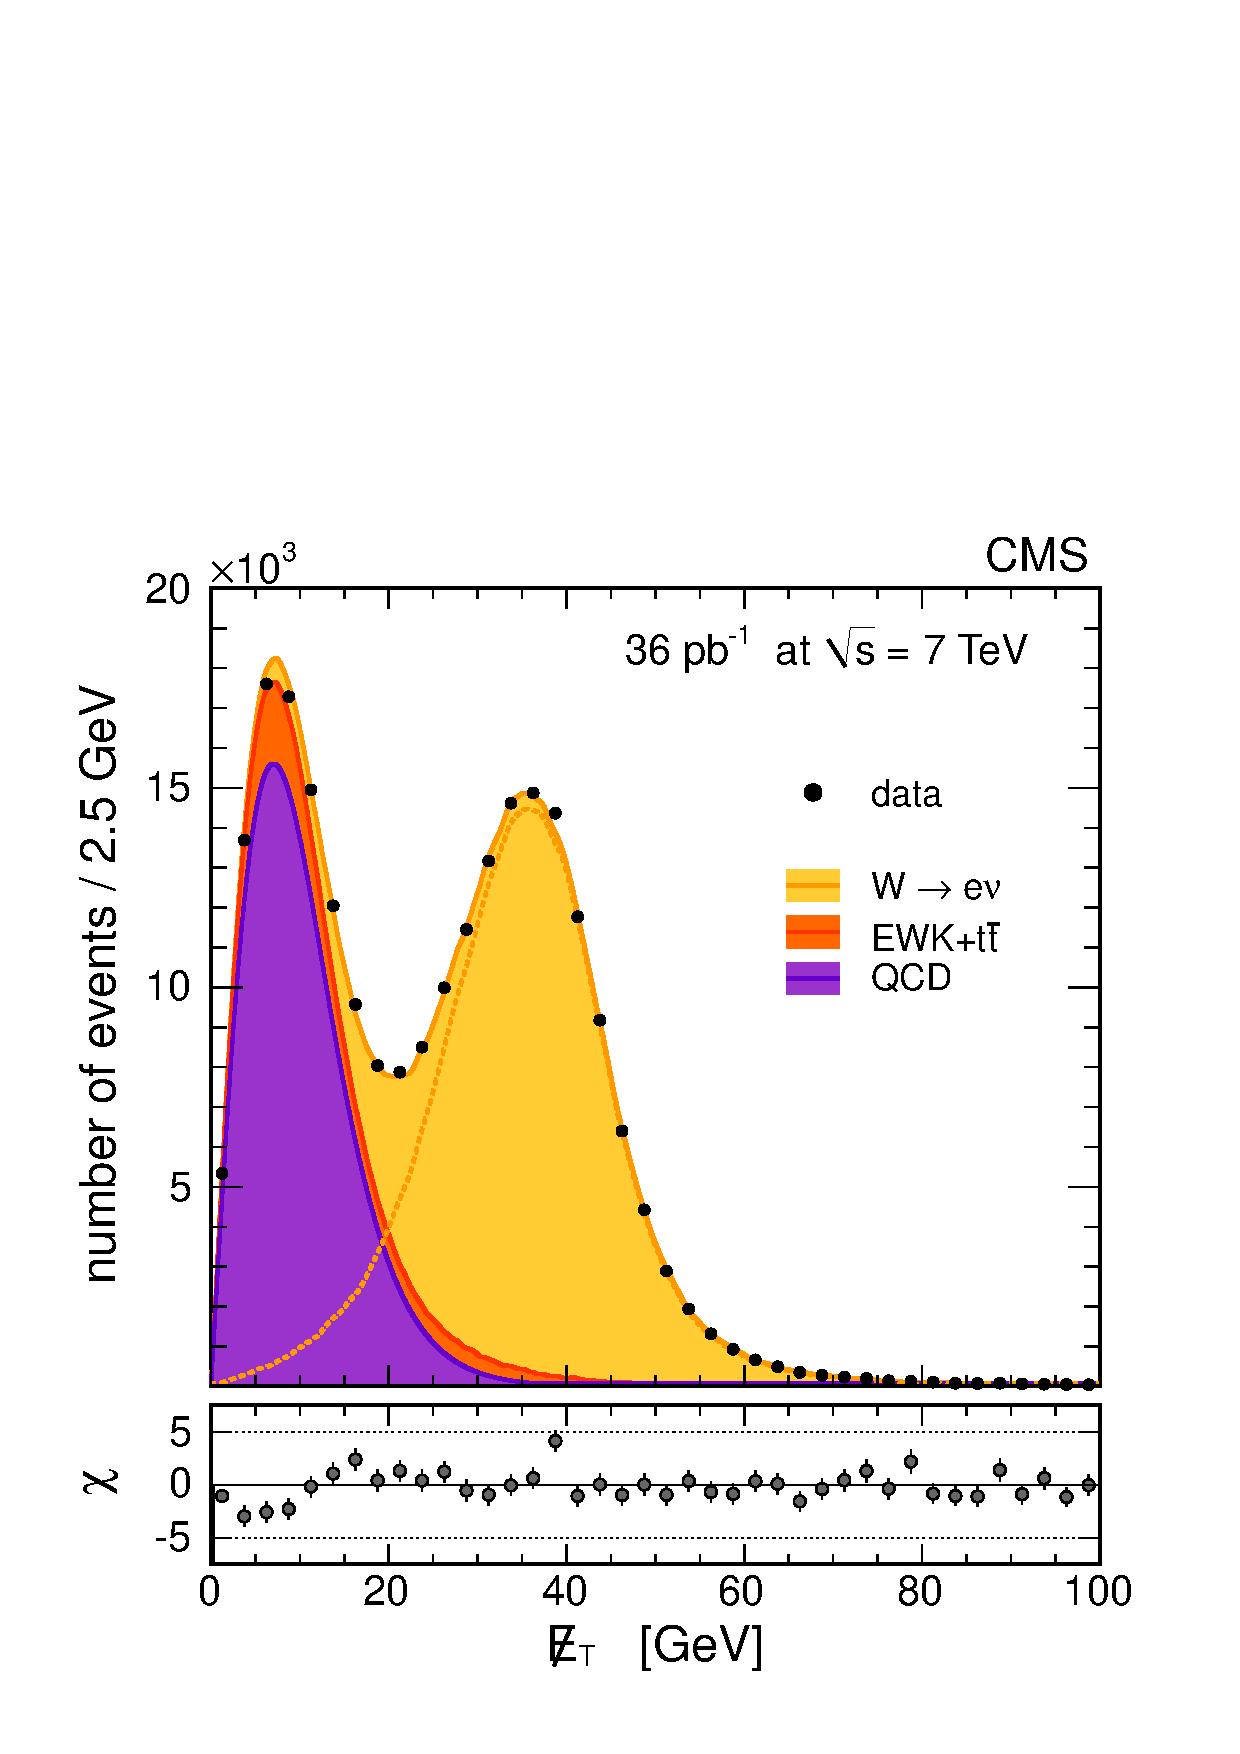
\includegraphics[width=0.48\textwidth]{figs/w_inc_36pb.pdf}
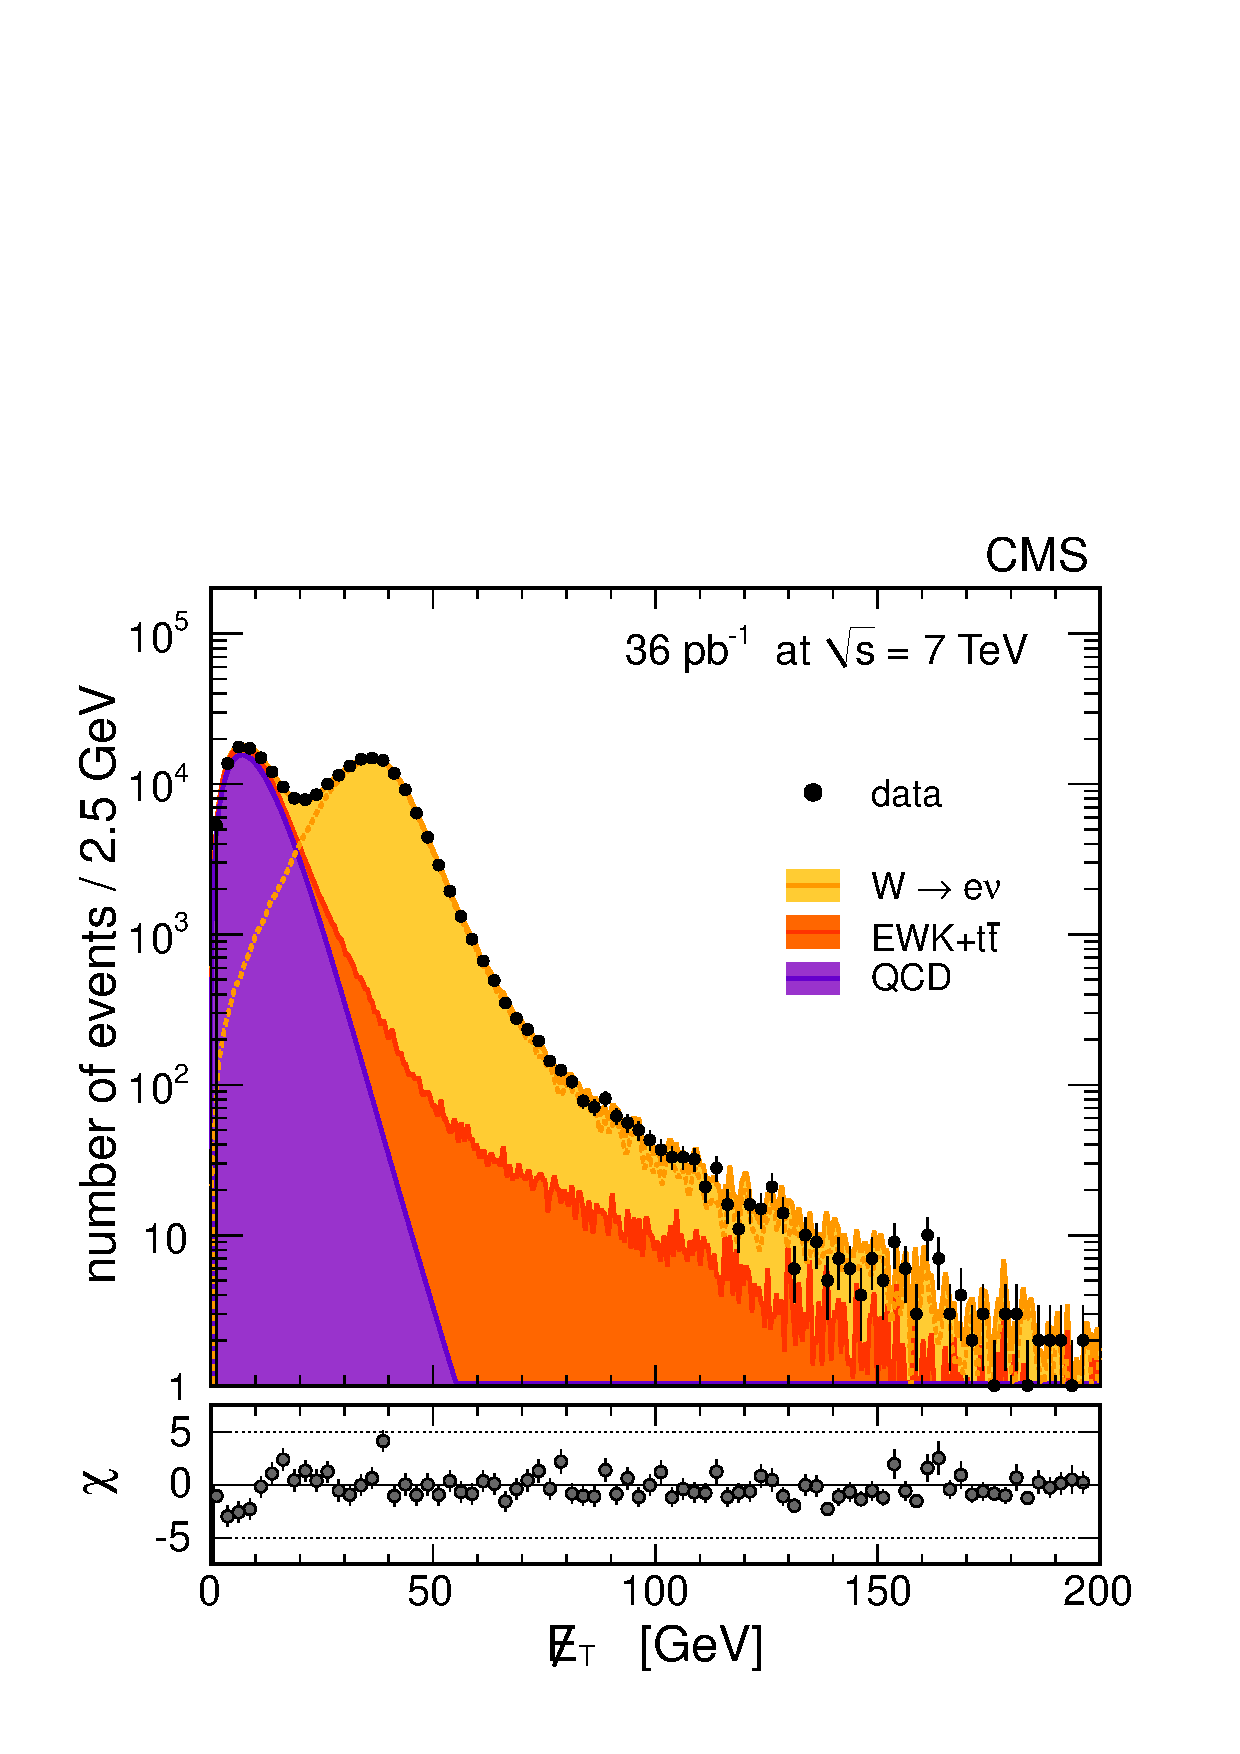
\includegraphics[width=0.48\textwidth]{figs/w_inc_36pb_log.pdf}
\caption{ \label{fig:Wen}
The $\MET$ distribution for the selected $\Wen$ candidates on
a linear scale (left) and on a logarithmic scale (right).
The points with the error bars represent the data. Superimposed are the
contributions obtained with the fit
for QCD background (violet, dark histogram), all other backgrounds
(orange, medium histogram), and signal plus  background (yellow, light histogram).
The orange dashed line is the fitted signal contribution.
}
\end{center}
\end{figure}

\begin{figure}[htbp]
\begin{center}
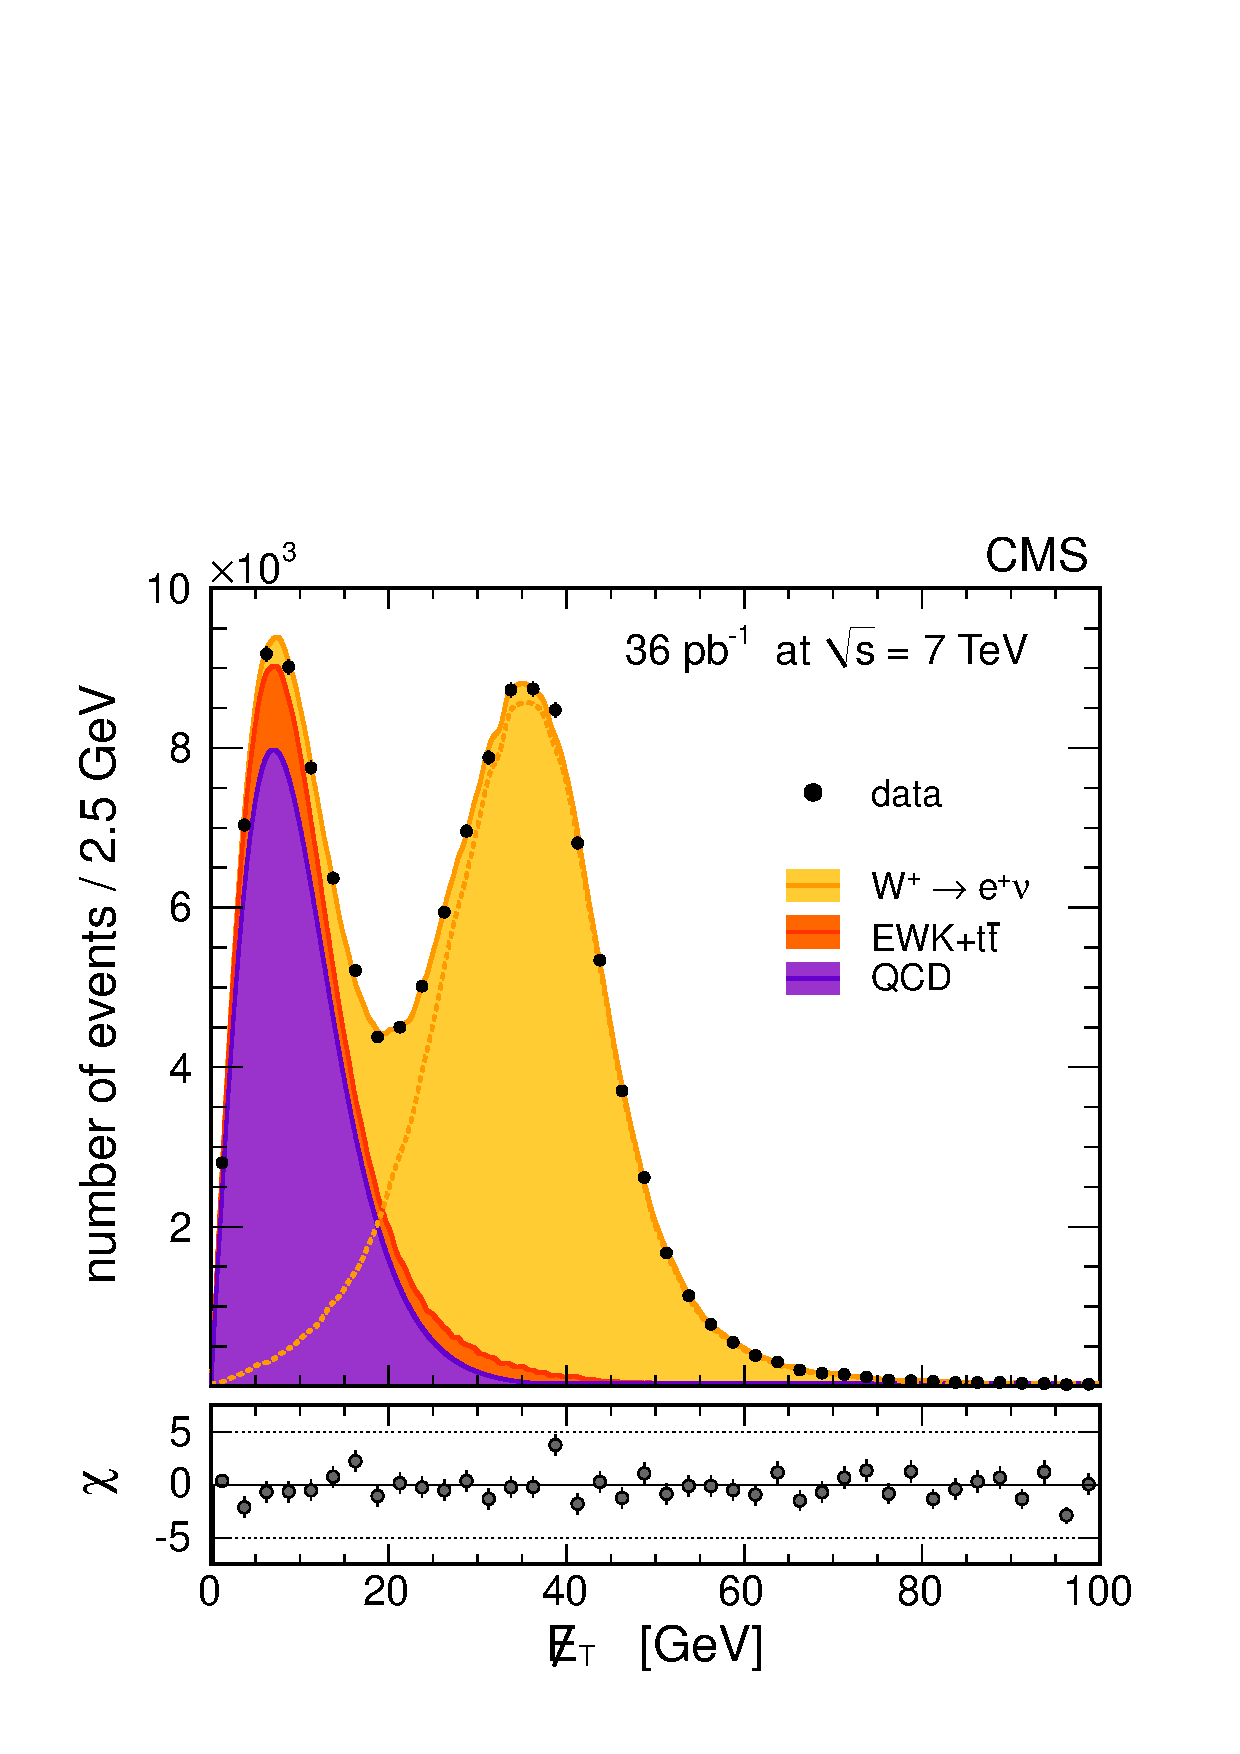
\includegraphics[width=0.48\textwidth]{figs/wp_36pb.pdf}
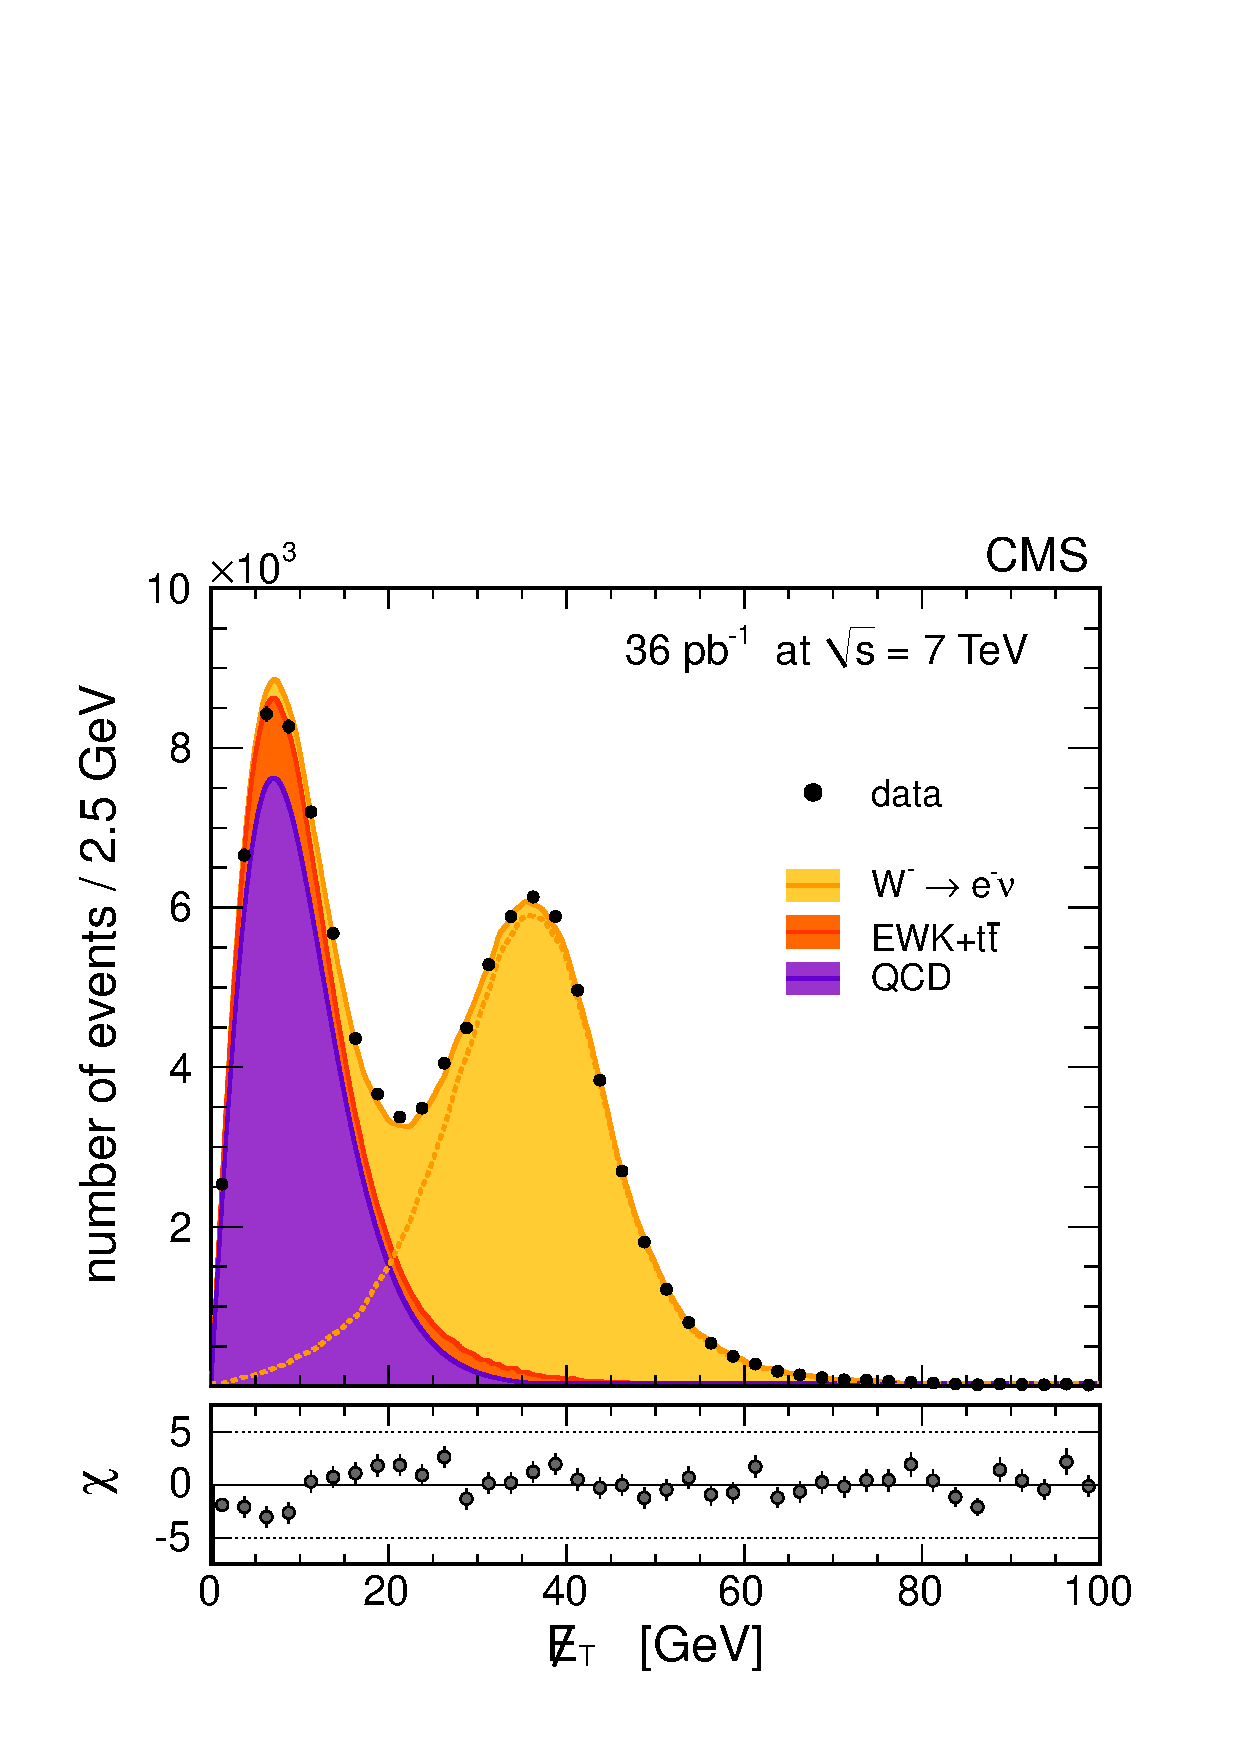
\includegraphics[width=0.48\textwidth]{figs/wm_36pb.pdf}
\caption{ \label{fig:WenPM}
The $\MET$ distributions for the selected W$^+$ (left) and W$^-$ (right) candidates.
The points with the error bars represent the data. Superimposed are the contributions
obtained with the fit for QCD background (violet, dark histogram), all other backgrounds
(orange, medium histogram), and signal plus background (yellow, light histogram).
The orange dashed line is the fitted signal contribution.
}
\end{center}
\end{figure}

The Kolmogorov--Smirnov probabilities for the fits to the charge-specific
channels are $\WEPKSPCOR$ for the $\Wp$ sample and
$\WEMKSPCOR$ for the $W^-$ sample.
\begin{figure}[t!]
\begin{center}
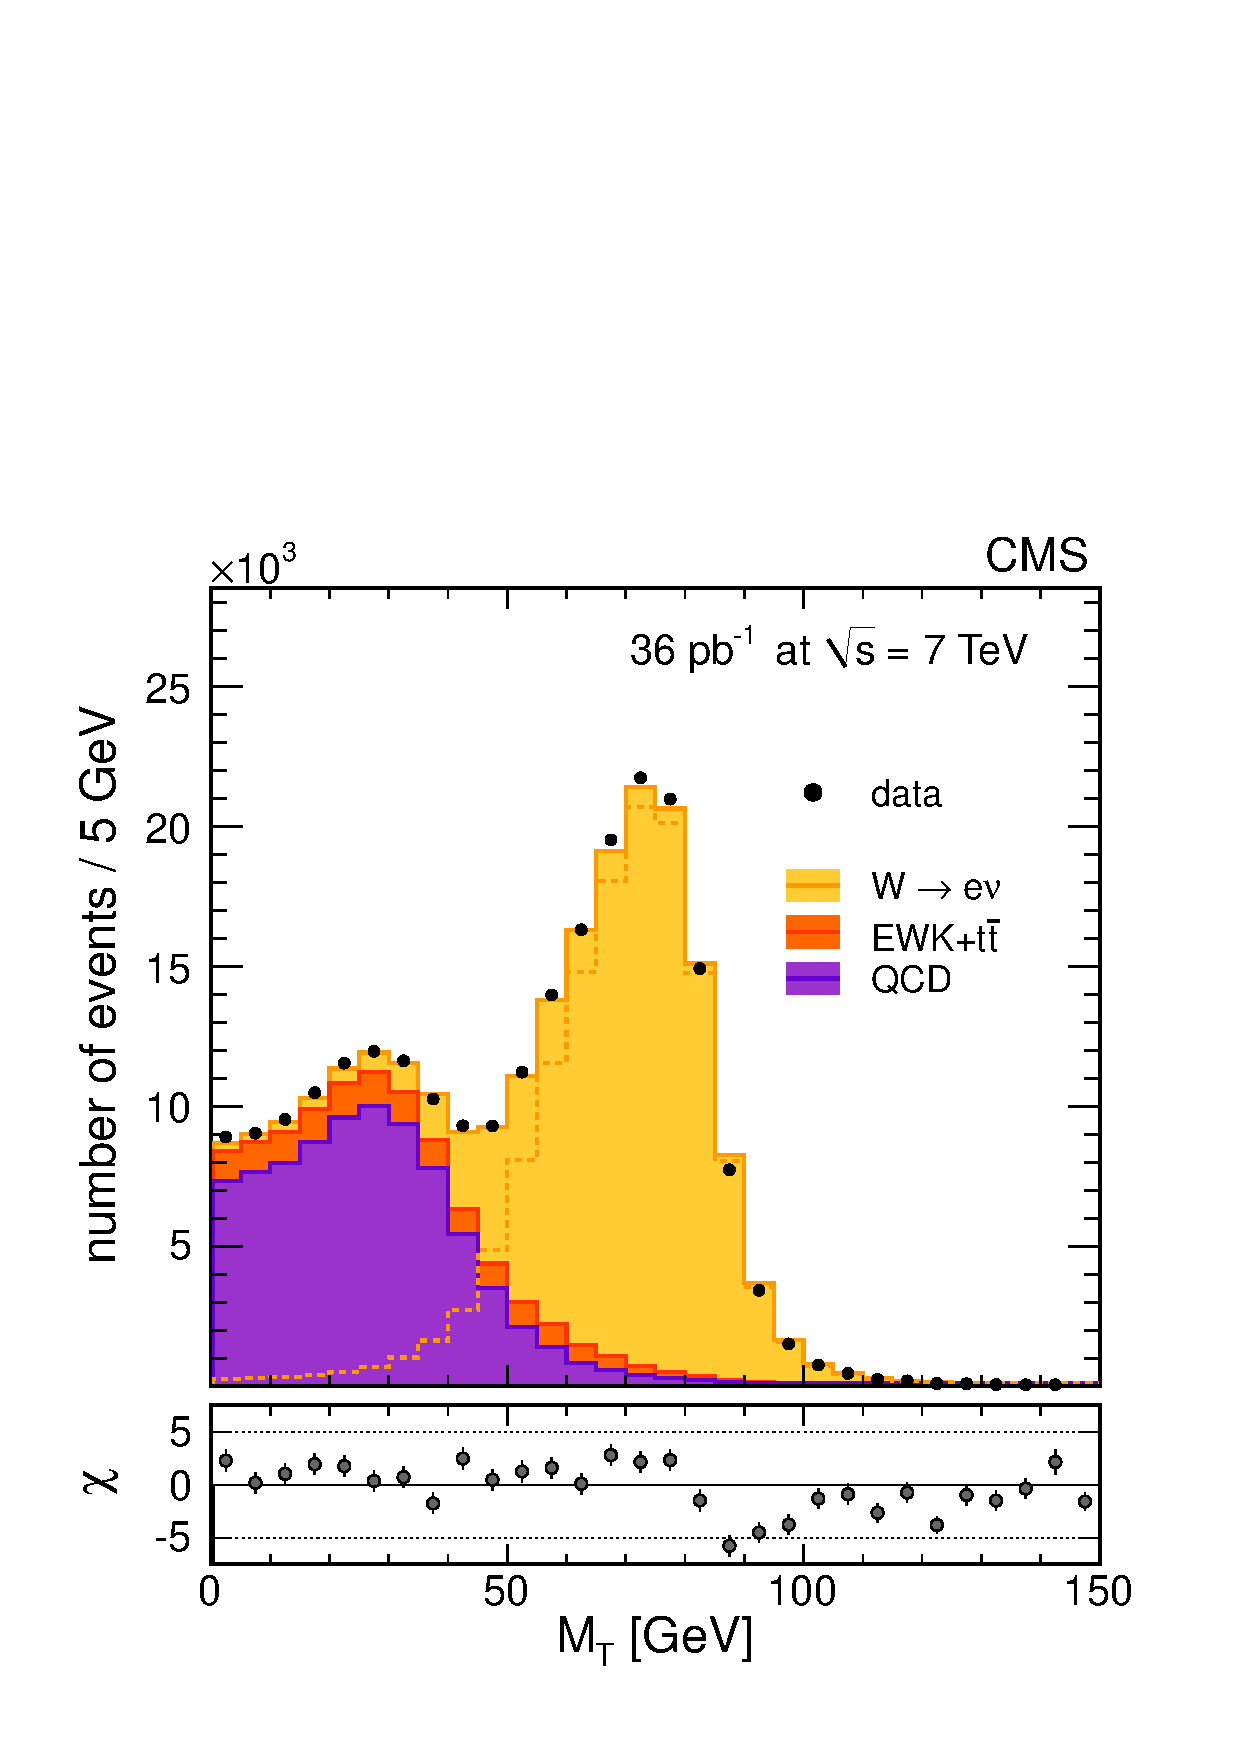
\includegraphics[width=0.48\textwidth]{figs/inc_pfmt_withMVA.pdf}
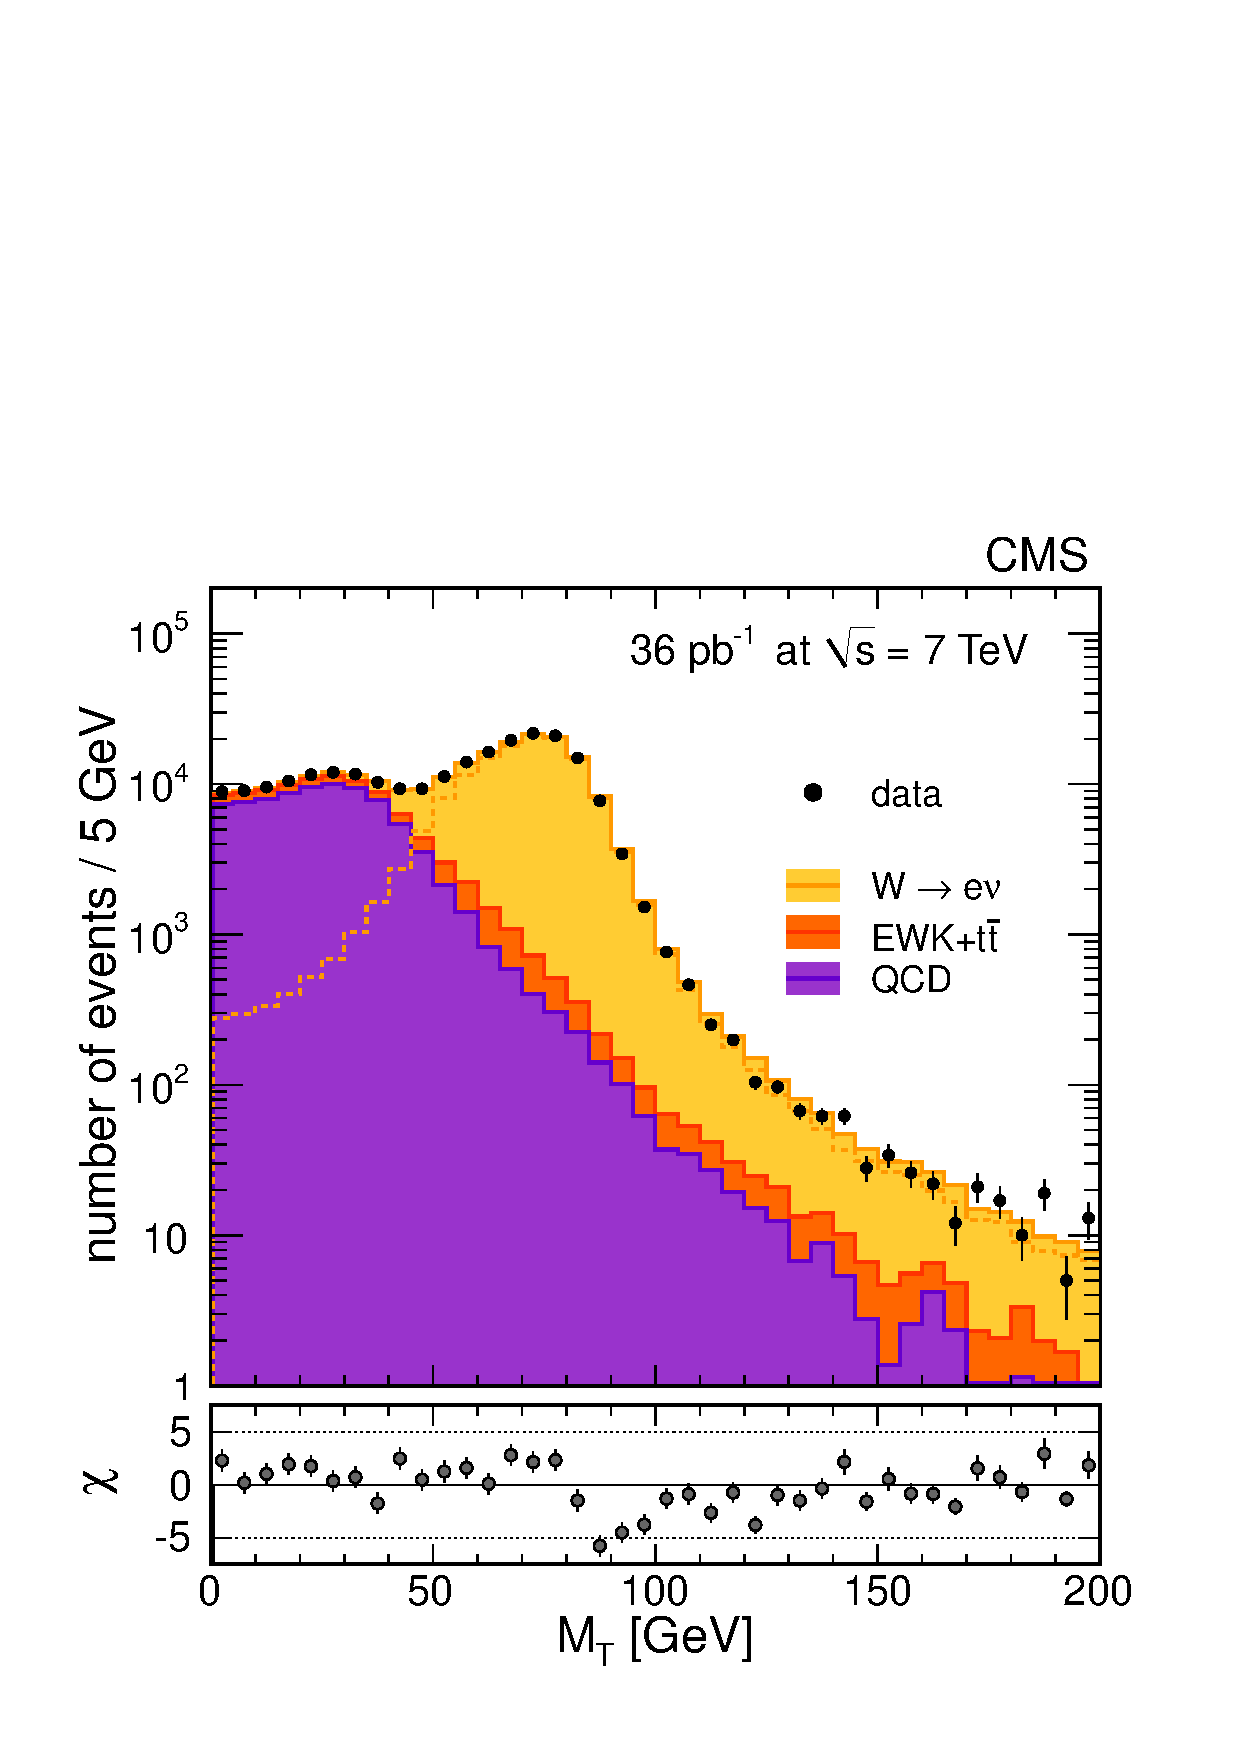
\includegraphics[width=0.48\textwidth]{figs/inc_pfmt_log_withMVA.pdf}
\caption{ \label{fig:WenMT}
The $\MT$ distribution for the selected $\Wen$ candidates on
a linear scale (left) and on a logarithmic scale (right).
The points with the error bars represent the data. Superimposed are the
contributions obtained with the fit
for QCD background (violet, dark histogram), all other backgrounds
(orange, medium histogram), and signal plus  background (yellow, light histogram).
The orange dashed line is the fitted signal contribution.
}
\end{center}
\end{figure}
Figure~\ref{fig:WenMT} shows the distribution for the inclusive $\Wo$ sample
of the transverse mass, defined as
$\MT=\sqrt{2\Pt\MET (1-\cos(\Delta\phi_{\mathrm{l},\MET}))}$,
where $\Delta\phi_{\mathrm{l},\MET}$ is the azimuthal angle between the
lepton and the $\MET$ directions.

\subsubsection{Modeling the QCD Background Shape with a Fixed Distribution}
\label{sec:e-Wsigextr-FixedTemplate}

In this approach the QCD shape is extracted directly from data using a 
control sample obtained by inverting a subset of the requirements used to select the 
signal. After fixing the shape from data,
only the normalization is allowed to float in the fit.  

The advantage of this approach 
is that detector effects, such as anomalous signals in the ca\-lo\-ri\-me\-ters or 
dead ECAL towers, are automatically reproduced in the QCD shape, since these 
effects are not affected by the selection inversion used to define the control sample.
The track-cluster matching variable $\Delta\eta$ is found
to have the smallest correlation with $\MET$ and is therefore chosen as the one 
to invert in order to suppress the signal and obtain the QCD control sample.  
Requirements on isolation and $H/E$ are the same as for the signal 
selection since these variables show significant correlation with \MET. 
\begin{figure}[h!]
  \begin{center}
    \includegraphics*[angle=-90,width=0.55\textwidth]{figs/antiselShape.pdf}
    \caption{Normalised \MET distribution for QCD and $\gamma$+jet simulated 
events passing the signal selection (solid histogram) compared 
to the normalised distribution for events from all simulated samples passing
the same inverted selection criteria used to obtain the control sample in data
(dashed histogram).}
    \label{fig:antiselShape}
  \end{center}
\end{figure}

The shape of the $\MET$ distribution for QCD and $\gamma$+jet simulated 
events passing the signal selection is compared 
to the \MET distribution for a simulated control sample composed of all simulated samples (signal and 
all backgrounds, weighted according to the 
theoretical production cross sections), after applying the same anti-selection 
as in data (Fig.~\ref{fig:antiselShape}).

\begin{figure}[htb]
  \begin{center}
    \includegraphics*[width=0.5\textwidth]{figs/Wenu_pfMET_lin.pdf}
%    \includegraphics*[width=0.48\textwidth]{figs/Wenu_pfMT_lin.pdf}
    \caption{Result of the fixed-shape fit to the $\MET$ distribution for all W candidates.
The points with the error bars represent the data.   Superimposed are the results
of the maximum likelihood fit for QCD background (violet, dark histogram), other backgrounds
(orange, medium histogram), and signal plus  background (yellow, light histogram).
The orange dashed line (left plot) is the fit contribution from signal.
}
    \label{fig:resultAll}
  \end{center}
\end{figure}

The difference in the $\MET$ distributions from the signal and inverted selections
is found to be predominantly due to two effects, which can be reduced by applying corrections.
The first effect is due to a large difference in the distribution of the output of a multivariate 
analysis (MVA) used for electron identification in the PF algorithm, between the selected events 
and the control sample. The value of the MVA output determines whether an electron candidate 
is treated by the PF algorithm as a genuine electron, or as a superposition of a charged pion and 
a photon, with track momentum and cluster energy each contributing separately to $\MET$. The control 
sample contains a higher fraction of electron candidates in the latter category, resulting in a bias on 
the $\MET$ shape. A correction is derived to account for this.
The second effect comes from the signal 
contamination in the control sample. The size of the contamination (1.17$\%$) is 
measured from data, using the \TNP technique with $\Zee$  
events, by measuring the efficiency for a signal electron to pass the 
control sample selection.


The results of the inclusive fit to the $\MET$ distribution with the fixed QCD background shape
are shown in Fig.~\ref{fig:resultAll}; the only free parameters in the extended 
maximum likelihood fit are the QCD and signal yields.
By applying this second method the following yields are obtained:
$135\,982 \pm 388$ (stat.) for the inclusive sample, $81\,286 \pm 302$ (stat.) for the $\Wpen$ sample, and
$54\,703 \pm 249$ (stat.) for the $\Wmen$ sample.
%with negligible correlation between the $\Wp$ and $\Wm$ yields.
%The quoted yields are from the $\MET$ fits. 
The ratios of the inclusive, $\Wpen$, and $\Wmen$ yields between this 
method and the parameterized
QCD shape method are $0.997 \pm 0.005$, $0.997 \pm 0.005$, and $0.999 \pm 0.005$, respectively, 
considering only the uncorrelated systematic uncertainties between the two methods.



\label{sec:e-Wsigextr-ABCDE}

\subsubsection{The ABCD Method}

%A brief summary of this method follows below. 
%A detailed description can be found 
%in the supporting document~\cite{CMS_AN_2011-009}.

In this method the data are divided into four categories defined by boundaries on $\MET$ and the relative tracker 
isolation, $\ITRK/\ET$, of the electron candidate. The boundaries of the regions are chosen to minimize the overall 
statistical and systematic uncertainties on the signal yield.
Values of $\MET$ above and below the boundary of 25 GeV, together with $\ITRK/\ET$ values below 
the boundary of 0.04, define the regions A and B, respectively.
\begin{figure}[htbp]
\begin{center}
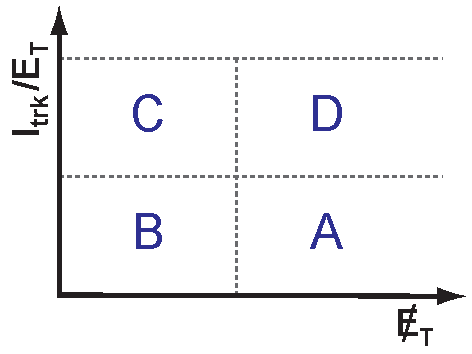
\includegraphics[width=0.35\textwidth]{figs/abcd.pdf}
\caption{The arrangement of the four categories of events used in the ABCD method. The vertical 
scale indicates increasing values of relative track isolation $\ITRK/\ET$
and the horizontal scale indicates increasing $\MET$.
%The dashed arrows show the directions of increasing signal purity.
}
\label{fig:abcde}
\end{center}
\end{figure}
Similarly, the regions above and below the $\MET$ boundary for $\ITRK/\ET$ values above 0.04, 
but below an upper $\ITRK/\ET$ bound of 0.2 (0.1) for electrons in the EB (EE), 
define the regions D and C, respectively. There is no upper bound for the $\MET$ values.
The different regions are shown graphically in Fig.~\ref{fig:abcde}, with region A 
having the greatest signal purity.
Combined regions are referred to as 'AB' (for A and B), for example.
The extracted signal corresponds to the entire ABCD region.

A system of equations is constructed relating the numbers of observed data events, $N_\mathrm{i}$, 
in each of the four regions ($\mathrm{i}$ = A, B, C and D) to the numbers 
of electroweak backgrounds, $E_\mathrm{i}$, QCD backgrounds, $Q_\mathrm{i}$, 
and signal events, $S_\mathrm{i}$. Several parameters should be determined from auxiliary 
measurements or simulations as shown in the following formulas: 

\begin{eqnarray}
 \label{eqABCD_Fa}
   f_\mathrm{A} & = & \frac{Q_\mathrm{A}}{Q_\mathrm{A} + Q_\mathrm{B}}  \\
  \label{eqABCD_Fb}
   f_\mathrm{D} & = & \frac{Q_\mathrm{D}}{Q_\mathrm{C} + Q_\mathrm{D}}  \\
  \label{eqABCD_EFFa}
   \epsilon_\mathrm{A} & = & \frac{S_\mathrm{A}}{S_\mathrm{A} + S_\mathrm{B}}  \\
  \label{eqABCD_EFFd}
   \epsilon_\mathrm{D} & = & \frac{S_\mathrm{D}}{S_\mathrm{C} + S_\mathrm{D}}  \\
  \label{eqABCD_EFFp}
   \epsilon_\mathrm{P} & = & \frac{S_\mathrm{A} + S_\mathrm{B}}{S_\mathrm{A} + S_\mathrm{B} + S_\mathrm{C} + S_\mathrm{D}} 
\end{eqnarray}

In this formulation, two parameters, $f_\mathrm{A}$ and $f_\mathrm{D}$, relate to the QCD 
backgrounds and are defined as the ratios of events with a fake electron candidate in the A and D 
regions to the number in the AB and CD regions, respectively. The two parameters represent the 
efficiency with which misidentified electrons pass the boundary on $\MET$ dividing
AD from BC. If the efficiency for passing the $\MET$ boundary is largely independent of the choice of
the boundaries on $\ITRK/\ET$, then these two parameters will be approximately equal. 
Assuming $f_\mathrm{A}=f_\mathrm{D}$ holds exactly 
leads to a simplification of the system of equations such that all direct dependence of the signal
extraction on parameters related to the QCD backgrounds is eliminated. For this idealized case there would be
no uncertainty on the extracted signal yield arising from modeling of QCD backgrounds. Detailed studies of the
data suggest this assumption holds to a good degree. A residual bias in the extracted signal arising from this
assumption is estimated directly from the data by studying a control sample 
obtained with inverted quality requirements on the electron candidate, 
and an appropriate small correction to the yield is applied (${\approx}0.37\%$).
A systematic uncertainty on the signal yield is derived from the uncertainty on this bias correction.
This contribution is small and is dominated by the uncertainty on signal
contamination in the control sample.

Three other important parameters relate to signal efficiencies: $\epsilon_\mathrm{A}$ 
and $\epsilon_\mathrm{D}$, which
are the efficiencies for signal events in the AB and CD regions, respectively, to pass the 
$\MET$ boundary, and $\epsilon_\mathrm{P}$, which is the efficiency for the electron candidate of a signal event 
to pass the boundary on relative track isolation dividing the AB region from the CD region under the 
condition that this electron already lies in the ABCD region. 
The first two of these, $\epsilon_\mathrm{A}$ and $\epsilon_\mathrm{D}$, are
estimated from models of the $\MET$ in signal events using the 
methods described in Section~\ref{sec:WsignalMETtemplate}.
The third parameter, $\epsilon_\mathrm{P}$, is measured from data using the \TNP method, described in
Section~\ref{sec:ELEefficiencies}, and is one of the dominant sources of 
uncertainty on the $\Wo$ boson yield before
considering the final acceptance corrections.

Electroweak background contributions are estimated from MC samples
with an overall normalization scaled through an iterative method with the signal yield. 
The electroweak contribution is subtracted from the observed data events in each of the four 
regions, $N_\mathrm{i} \rightarrow N_\mathrm{i} - E_\mathrm{i}$ ($\mathrm{i}$ = A, B, C and D).

Assuming that $f_\mathrm{A}$ = $f_\mathrm{B}$, the signal contained in the ABCD region, S, can 
be obtained from the following formula:

\begin{eqnarray}
 \label{eqABCD_S}
   \alpha S^2 + b S + c & = & 0 
\end{eqnarray}

with coefficients, 

\begin{eqnarray}
 \label{eqABCD_Sa}
   \alpha & = & \epsilon_\mathrm{P}(\epsilon_\mathrm{P} - 1)(\epsilon_\mathrm{A} - \epsilon_\mathrm{D})   \\
  \label{eqABCD_Sb}
   b & = & N_\mathrm{A}(1 - \epsilon_\mathrm{D})(1 - \epsilon_\mathrm{P}) - N_\mathrm{B}\epsilon_\mathrm{D}(1 - \epsilon_\mathrm{P}) + N_\mathrm{C}\epsilon_\mathrm{A}\epsilon_\mathrm{P} - N_\mathrm{D}\epsilon_\mathrm{P}(1 - \epsilon_\mathrm{A})  \\
  \label{eqABCD_Sc}
   c & = & N_\mathrm{B}N_\mathrm{D} - N_\mathrm{A}N_\mathrm{C}
\end{eqnarray}

The extracted yield with respect to the choice of boundaries in relative track isolation and $\MET$ is 
sensitive to biases in $\epsilon_\mathrm{P}$ and the QCD electron misidentification rate 
bias correction described above, respectively. 
The yield is very stable with respect to small changes in these selections, 
giving confidence that these 
important sources of systematic uncertainty are small.

The following signal yields are obtained:
$136\,003 \pm 498\,\mathrm{(stat.)}$ for the inclusive sample, $81\,525 \pm 385\,\mathrm{(stat.)}$ 
for the $\Wpen$ sample, and $54\,356 \pm 315\,\mathrm{(stat.)}$ for the $\Wmen$ sample.
%with negligible correlation between the $\Wp$ and $\Wm$ yields.
The ratios of the inclusive, $\Wpen$, and $\Wmen$ yields between this method and the parameterized
QCD shape are $0.998 \pm 0.007$, $0.999 \pm 0.007$, and $0.993 \pm 0.007$, respectively, considering
only the uncorrelated systematic uncertainties between the two methods.



The results of the three signal extraction methods are summarised in Table~\ref{tab:WsignalCollection}.

\begin{table}[htbp] %
\begin{center}
   \caption[.]{ \label{tab:WsignalCollection}
Comparison of $\Wen$ signal extraction methods. The signal yield of each method is presented together with
its statistical uncertainty.
For the fixed shape and the ABCD methods, the ratios of the signal yields with the analytical function method
are also shown taking into account only the uncorrelated systematics between the methods used in the ratios.}
\begin {tabular} {|l|l|c|c|c|}
\hline
\multicolumn{2}{|l|}{Source}        & $\Wen$           & $\Wpen$           & $\Wmen$            \\
\hline\hline
Analytical fun. &yield    & $\WEIYIELD$      &  $\WEPYIELD$      &  $\WEMYIELD$      \\
\hline
\multirow{2}{*}{Fixed shape} & yield                         & $\WEIftYIELD$    &  $\WEPftYIELD$    &  $\WEMftYIELD$      \\
 & ratio & $\rWEIftYIELD$   &  $\rWEPftYIELD$   &  $\rWEMftYIELD$      \\
\hline
\multirow{2}{*}{ABCD} & yield                                & $\WEIabYIELD$    & $\WEPabYIELD$     & $\WEMabYIELD$    \\
 & ratio       & $\rWEIabYIELD$   & $\rWEPabYIELD$    & $\rWEMabYIELD$    \\
\hline
\end {tabular}
\end{center}
\end{table}



\subsection{\texorpdfstring{Modeling of the QCD Background and $\Wmn$ Signal Yield}{Modeling of the QCD Background the W->mu nu Signal Yield}}
\label{sec:Wmunu}

The $\Wmn$ analysis is performed using fixed distributions for the $\MET$ shapes
obtained from data for the QCD background component and from simulations,
after applying proper corrections, for the signal and the remaining background components.

Different approaches to signal extraction are considered for $\Wmn$, as for $\Wen$.
The alternative methods do not demonstrate better performance than the use of fixed shapes
in the W signal fit. Given the lower backgrounds in the muon channel with respect to the
electron channel, the alternative strategies are not pursued at the same level of detail
as in the electron case.

The $\MET$ shape of the QCD background component is obtained from a high-purity QCD sample
of events that pass the signal selection, except that the isolation requirement
is inverted and set to $\IRelComb > 0.2$ (Fig.~\ref{figure:Wmunu_iso}).

Simulation studies indicate that this distribution does not accurately
reproduce the $\MET$ shape when muon isolation is required.
This is shown in Fig.~\ref{figure:Wmunu_QCD} (left),
where the solid line represents the shape for events with an isolated muon and the dashed line
the shape obtained by inverting the isolation requirement. %They are very distinct.

A positive correlation between the isolation variable $\IRelComb$ and $\MET$ is shown
in Fig.~\ref{figure:Wmunu_QCD} (right, red open circles). This behavior can be
parameterized in terms of a linear function
$\MET\propto (1+\alpha\,\IRelComb)$, as shown in the same figure.
A compensation for the correlation is subsequently made
by applying a correction of the kind of $\MET^\prime = \MET/(1+\alpha\,\IRelComb)$ to
the events selected by inverting the isolation requirement and a new corrected shape is obtained.
The agreement of this new shape (black points in Fig.~\ref{figure:Wmunu_QCD}, left)
with the prediction from events with an isolated muon is considerably improved.
It is also observed that a maximal variation in the correction factor of $\Delta \alpha =  0.08$ successfully
covers the simulation prediction for events with an isolated muon over the whole $\MET$ interval (shaded area in Fig.~\ref{figure:Wmunu_QCD}, left).
\begin{figure}[htbp] {\centering
    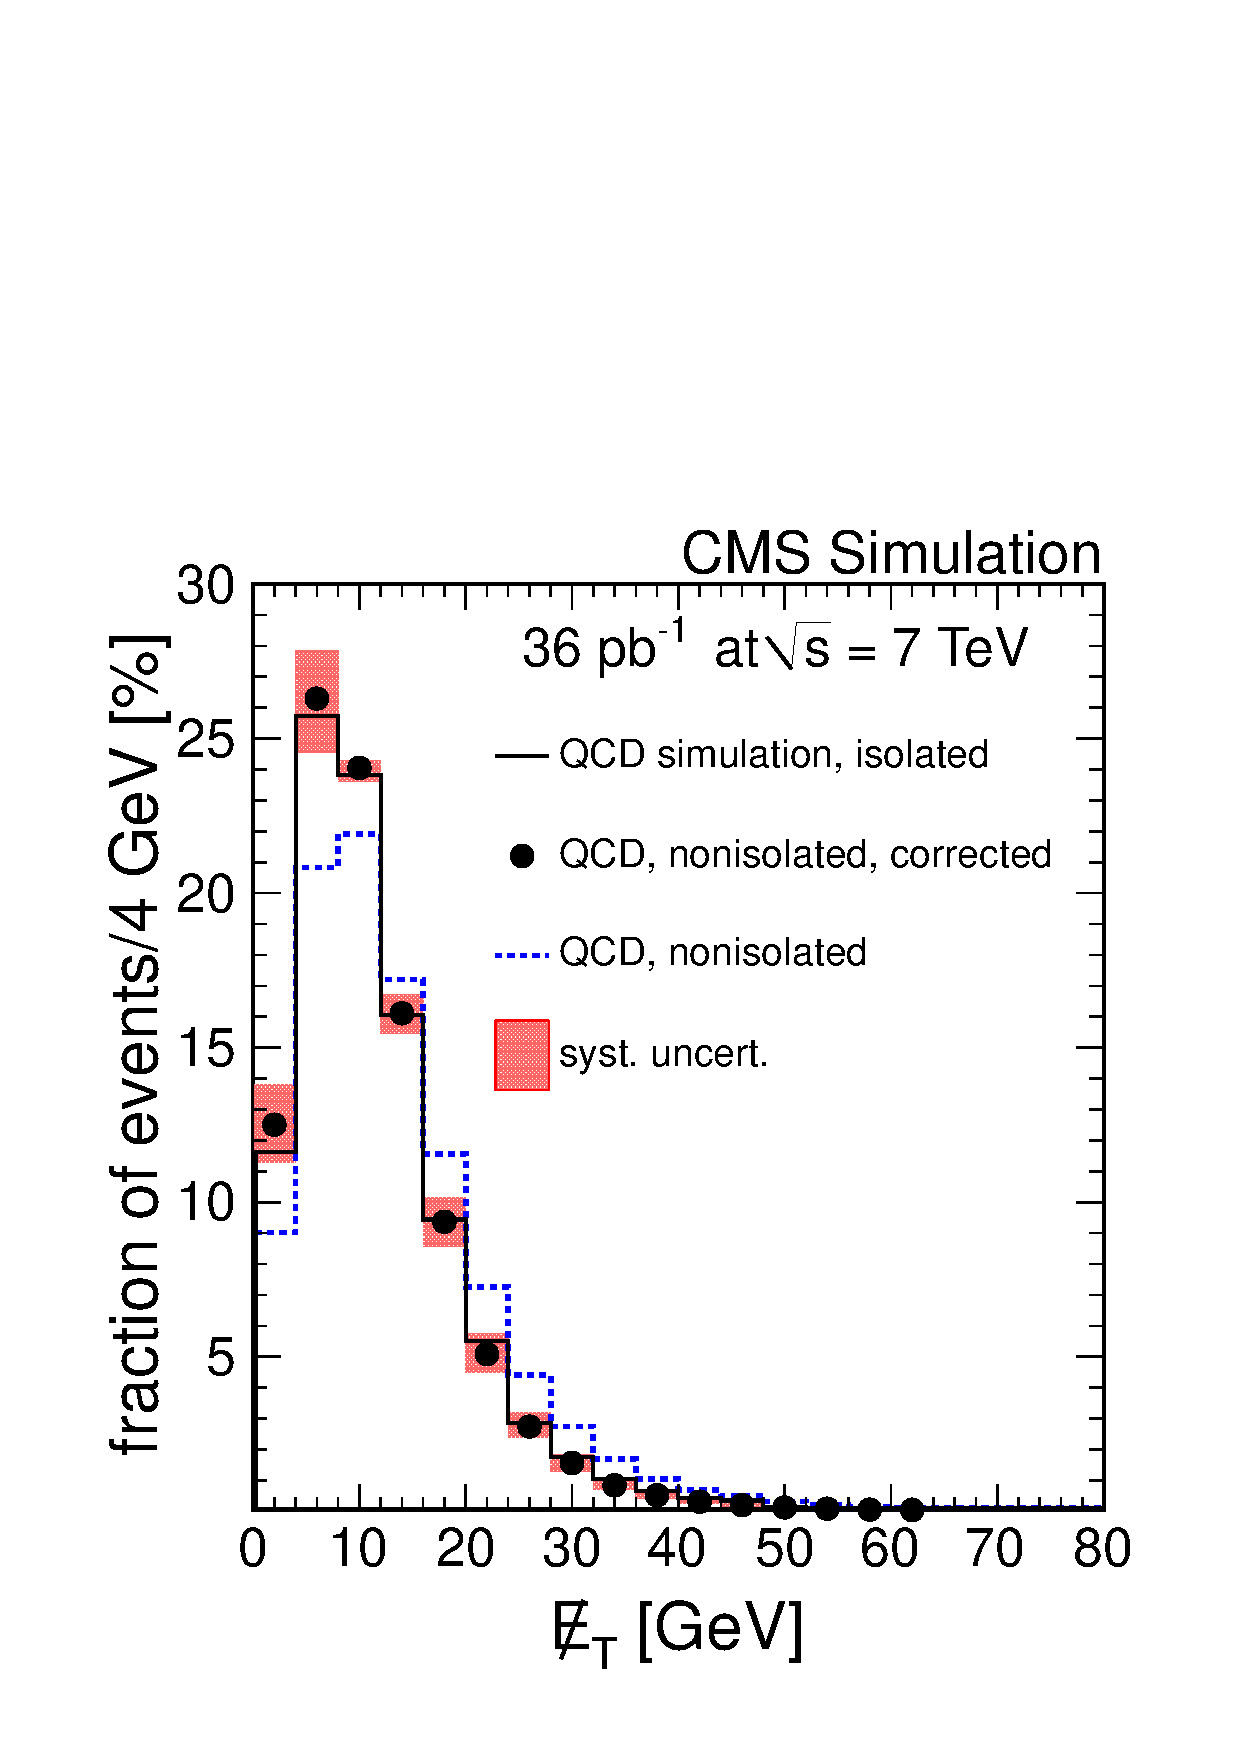
\includegraphics[width=7.5cm]{figs/qcd_template_MC.pdf}
    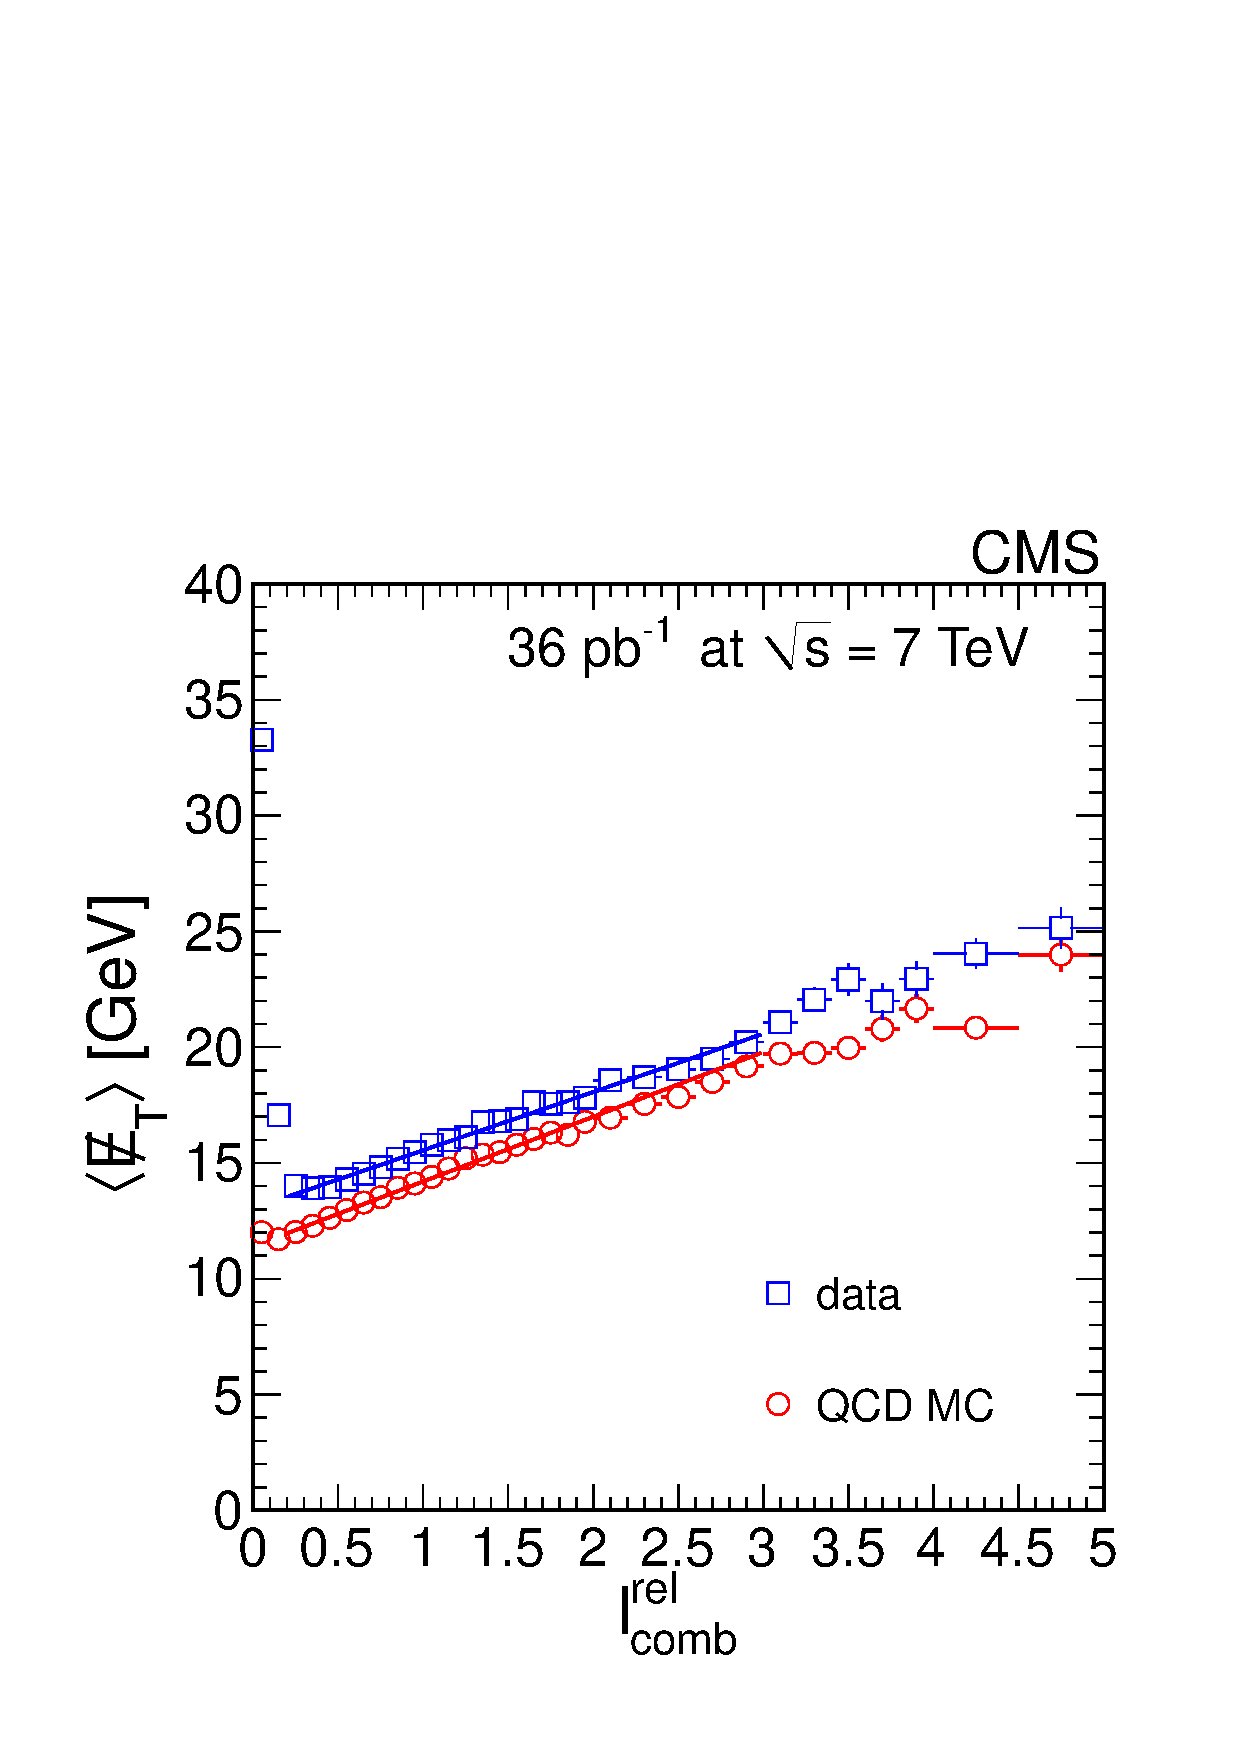
\includegraphics[width=7.5cm]{figs/Wmn_METvsIso.pdf}
    \caption{Left: distribution of the corrected $\MET$ for selected events
with a non isolated muon (black points) superimposed
on the distribution of uncorrected $\MET$ for the same events (blue, dashed line) and
$\MET$ for events with an isolated muon (black, solid histogram). All distributions are from simulated QCD events.
The shaded area represents the systematic uncertainty due to corrections
with factors $\alpha \pm \Delta \alpha$, for $\Delta \alpha = 0.08$.
Right: distribution of the average $\MET$ versus $\IRelComb$
for simulated QCD events (red circles) and
for data (blue squares).
The high values of $\MET$ in the first two bins in $\IRelComb$
are due to the presence of the W signal events. The superimposed lines are linear fits
in the range $[0.2, 3.0]$ of $\IRelComb$.
    \label{figure:Wmunu_QCD}}
}
\end{figure}
\begin{figure}[htbp]
{\centering
    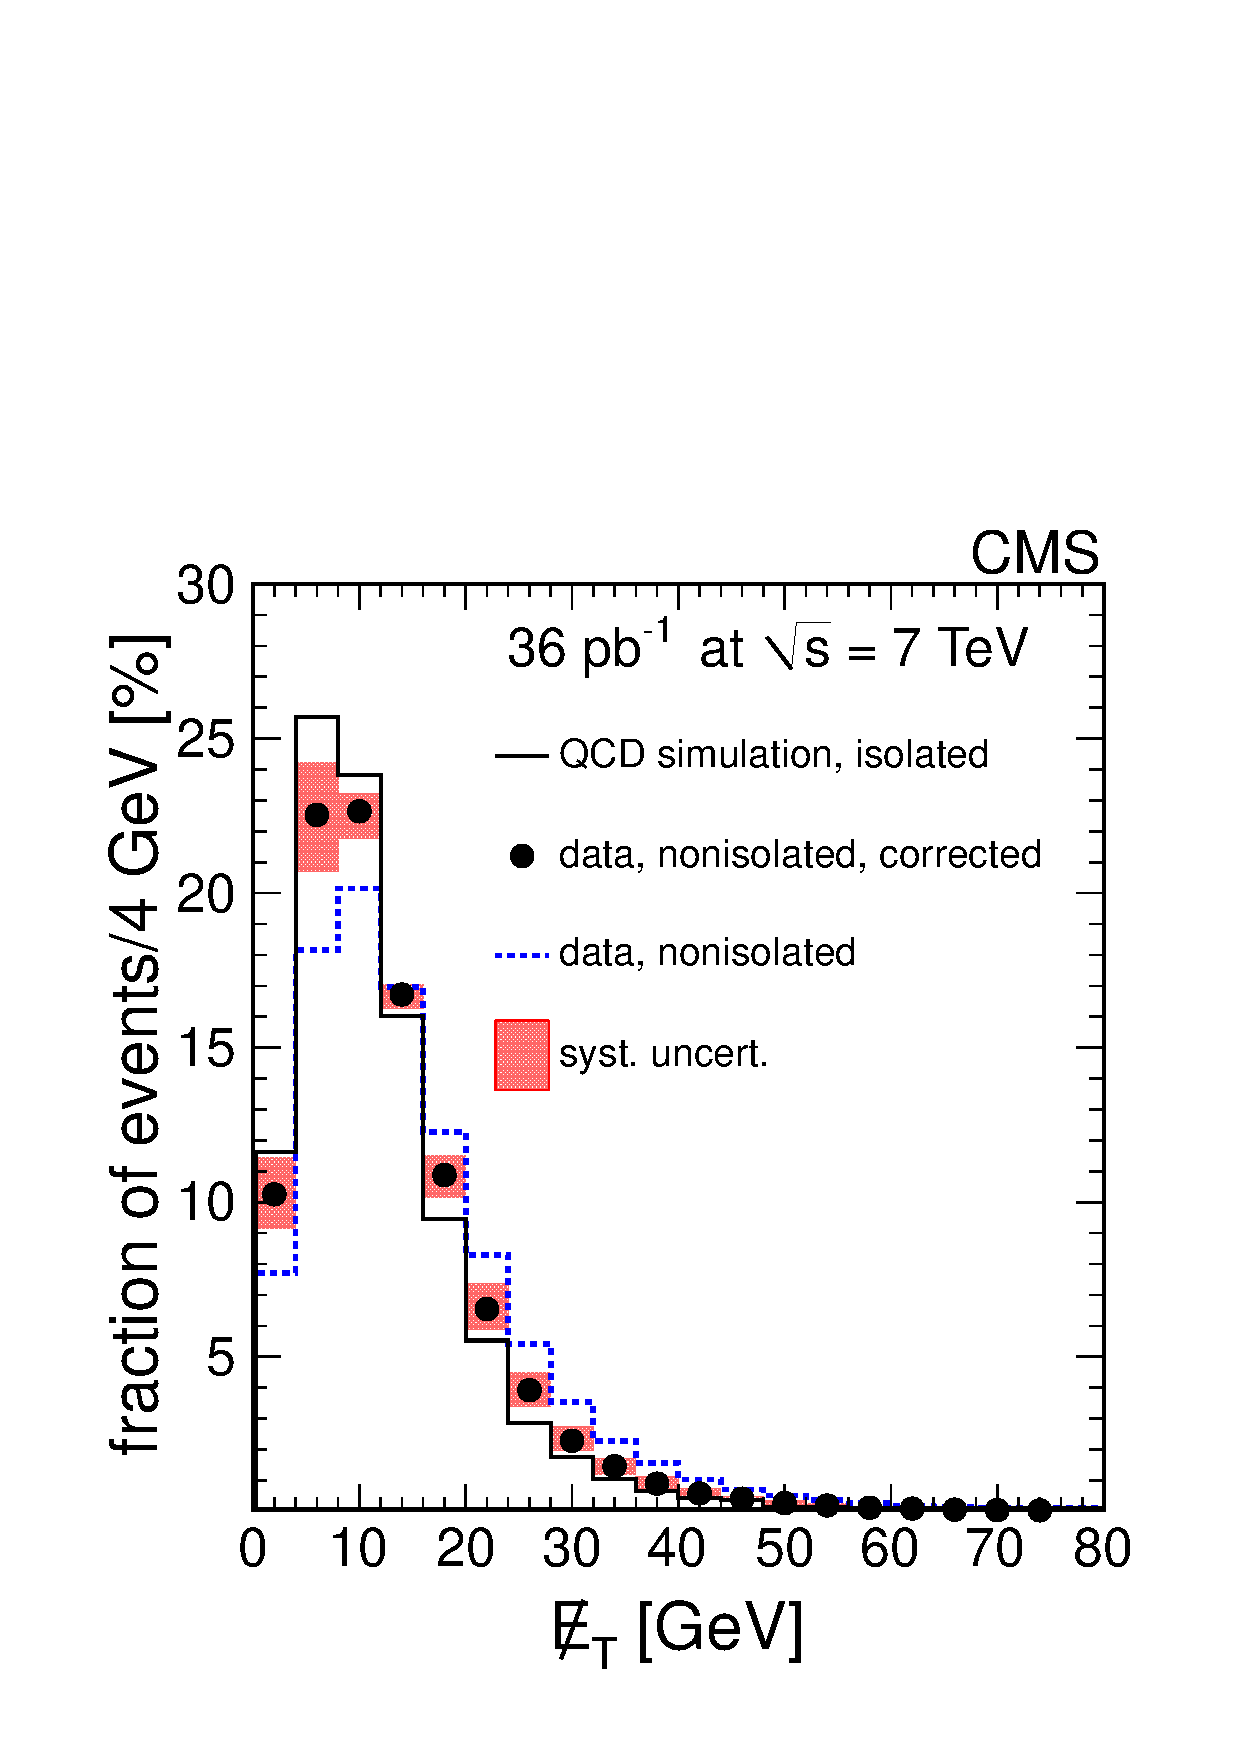
\includegraphics[width=7.5cm]{figs/qcd_template.pdf}
    \caption{
Distribution of the corrected $\MET$ for selected events
with a nonisolated muon in data (black points) superimposed
on the uncorrected $\MET$ distributions for data (blue dashed line) and
simulated QCD events (black, solid histogram, same as
the black, solid histogram in Fig.~\ref{figure:Wmunu_QCD}).
The shaded area represents the systematic uncertainty due to corrections with factors
$\alpha \pm \Delta \alpha$ for $\Delta \alpha = 0.08$.
    \label{figure:Wmunu_QCD_data}}
}
\end{figure}

The same positive correlation between $\MET$ and $\IRelComb$ is observed in the data
(blue squares in Fig.~\ref{figure:Wmunu_QCD}, right).
A correction $\MET^\prime = \MET/(1+\alpha\,\IRelComb)$, with $\alpha \approx 0.2$,
was applied.
The shapes obtained in data are shown in Fig.~\ref{figure:Wmunu_QCD_data} where
the uncorrected and corrected data shapes from events selected by inverting the isolation requirement, together with the
simulation expectation for events with an isolated muon, are shown.
The shaded area in Fig.~\ref{figure:Wmunu_QCD_data} is bounded by the two distributions, obtained using two extreme correction
parameters $\alpha \pm \Delta \alpha$, with $\Delta \alpha = 0.08$, as evaluated in simulations.
This area is taken as a systematic uncertainty on the QCD background shape.

Several parameterizations for the correction are considered,
but the impact on the corrected distribution and therefore on the final result is small.
Associated uncertainties on the cross section and ratios are evaluated as the differences between
the fit results obtained with the optimal $\alpha$ value and
two extreme cases, $\alpha \pm \Delta \alpha$.


The following signal yields are obtained: $140\,757 \pm 383$ for the inclusive sample,
$56\,666\pm240$ for the $\Wmmn$ sample, and $84\,091\pm291$ for the $\Wpmn$ sample.

The $\MET$ distributions are presented in
Fig.~\ref{figure:Wmunu_exp_fit} (full sample) and Fig.~\ref{figure:Wmn_PlusMinus}
 (samples selected by the muon charge) superimposed on the individual fitted
contributions of the W signal and the EWK and QCD backgrounds.
Figures~\ref{figure:Wmunu_exp_fit} and~\ref{figure:Wmn_PlusMinus}
show the $\MET$ distributions for data and fitted signal, plus background components.
 Figure~\ref{figure:Wmunu_exp_fit_mt}
% and~\ref{figure:Wmn_PlusMinus_mt}
shows the $\MT$ distributions for data and signal, plus background components, fitted
from the $\MET$ spectra.

% The fitted W parameters are summarized in Tables~\ref{table:Wmunu_tot_xs}
% for the two choices of fit parameters. The error shown is only statistical.
 \begin{figure}[!ht] {\centering
   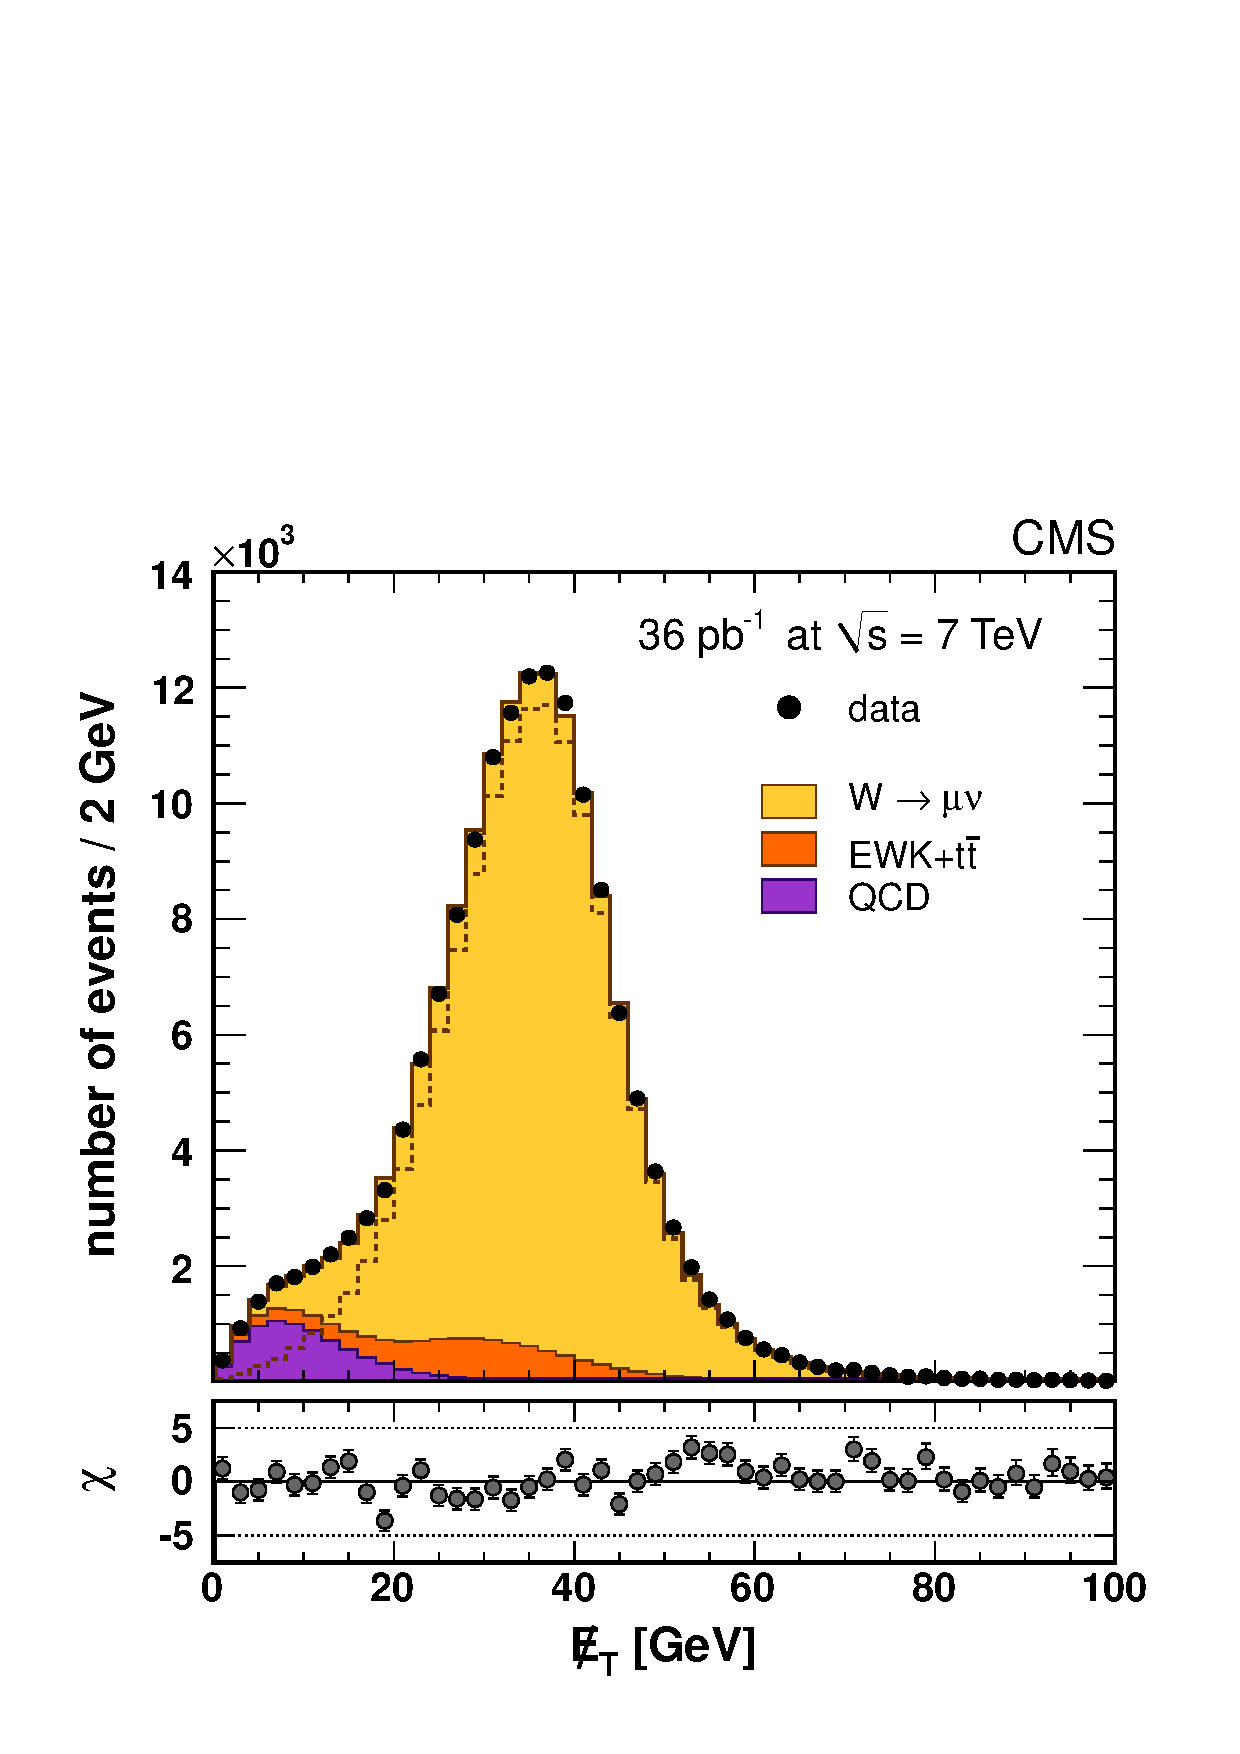
\includegraphics[width=7cm]{figs/Wmn_MET.pdf}
   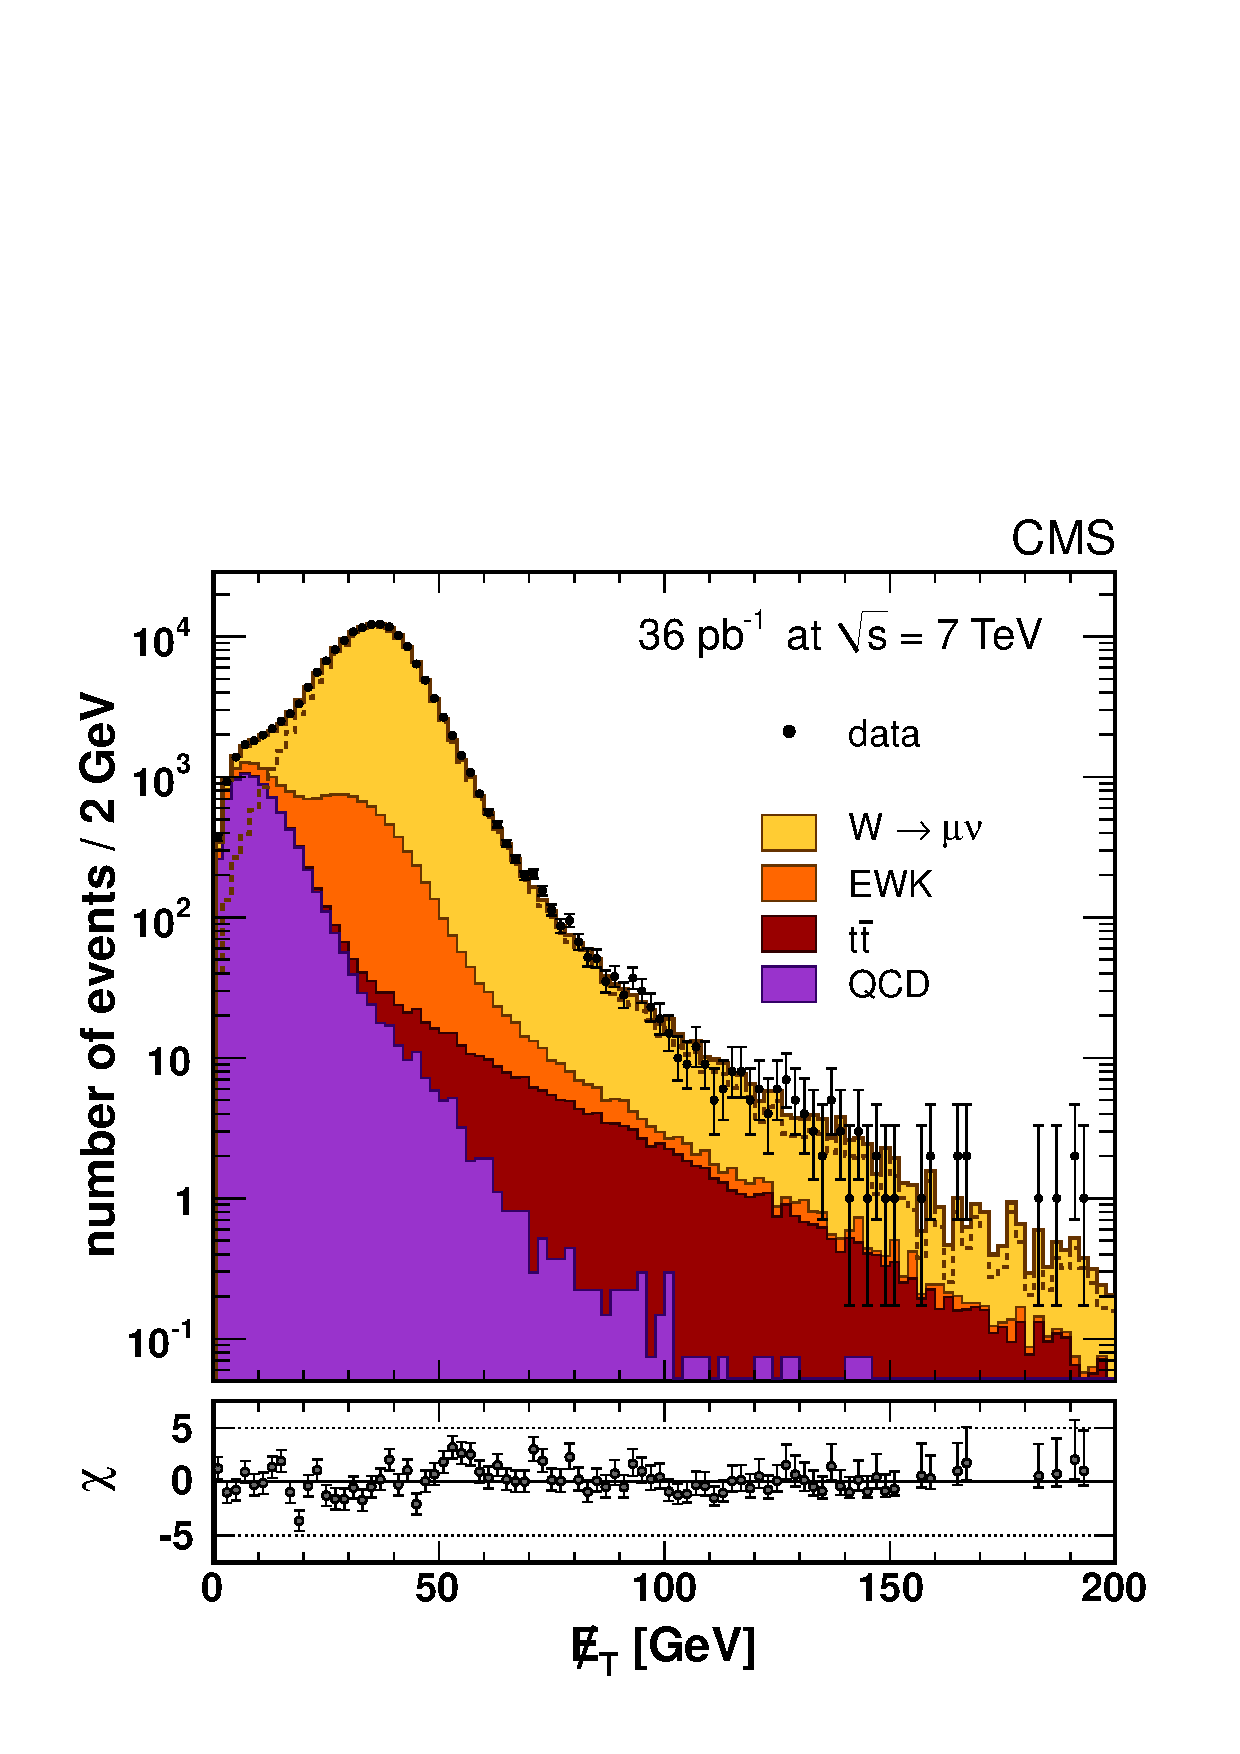
\includegraphics[width=7cm]{figs/Wmn_MET_log.pdf}
     \caption{
The $\MET$ distribution for the selected $\Wmn$ candidates on
a linear scale (left) and on a logarithmic scale (right).
The points with the error bars represent the data. Superimposed are the
contributions obtained with the fit
for QCD background (violet, dark histogram), all other backgrounds
(orange, medium histogram), and signal plus  background (yellow, light histogram).
The black dashed line is the fitted signal contribution.
     \label{figure:Wmunu_exp_fit}}
}
 \end{figure}

\begin{figure}[!ht] {\centering
   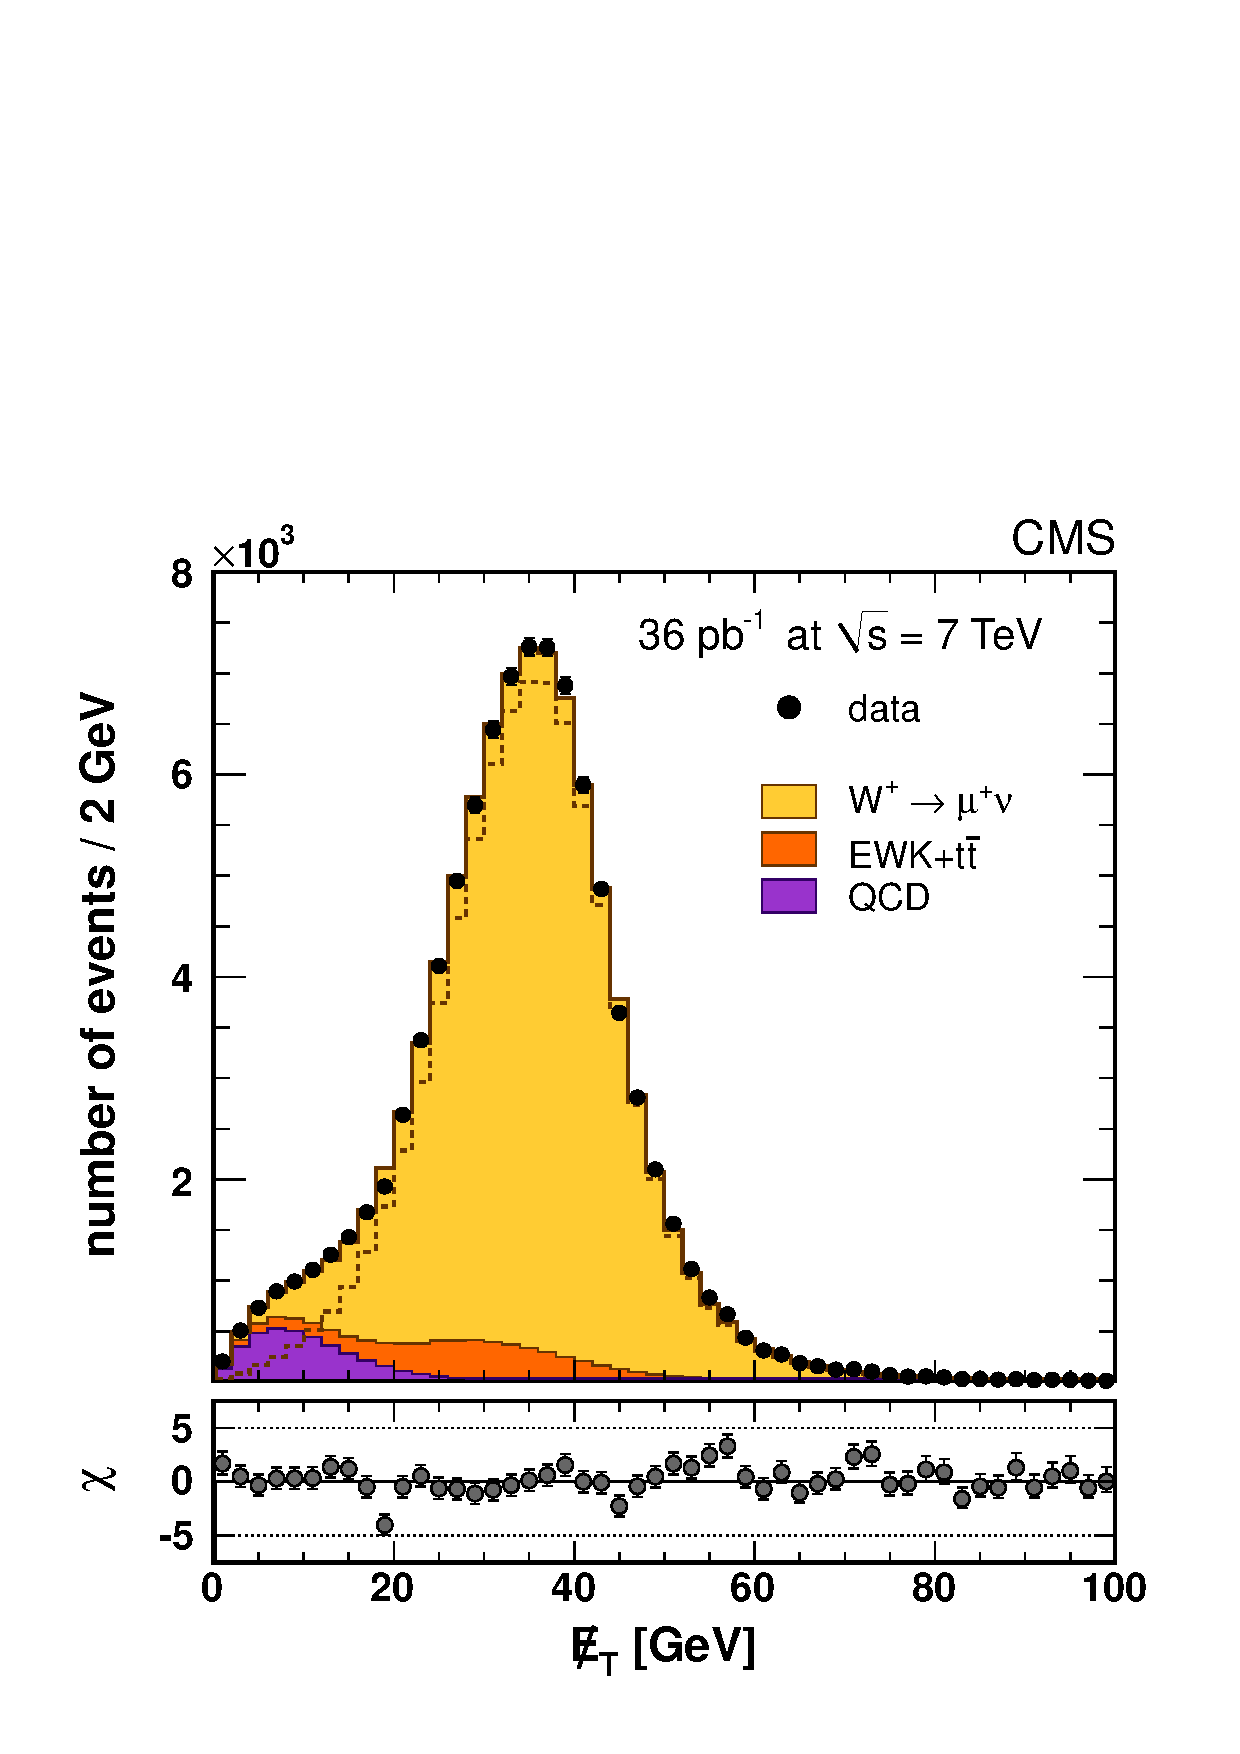
\includegraphics[width=7cm]{figs/Wmn_MET_plus.pdf}
   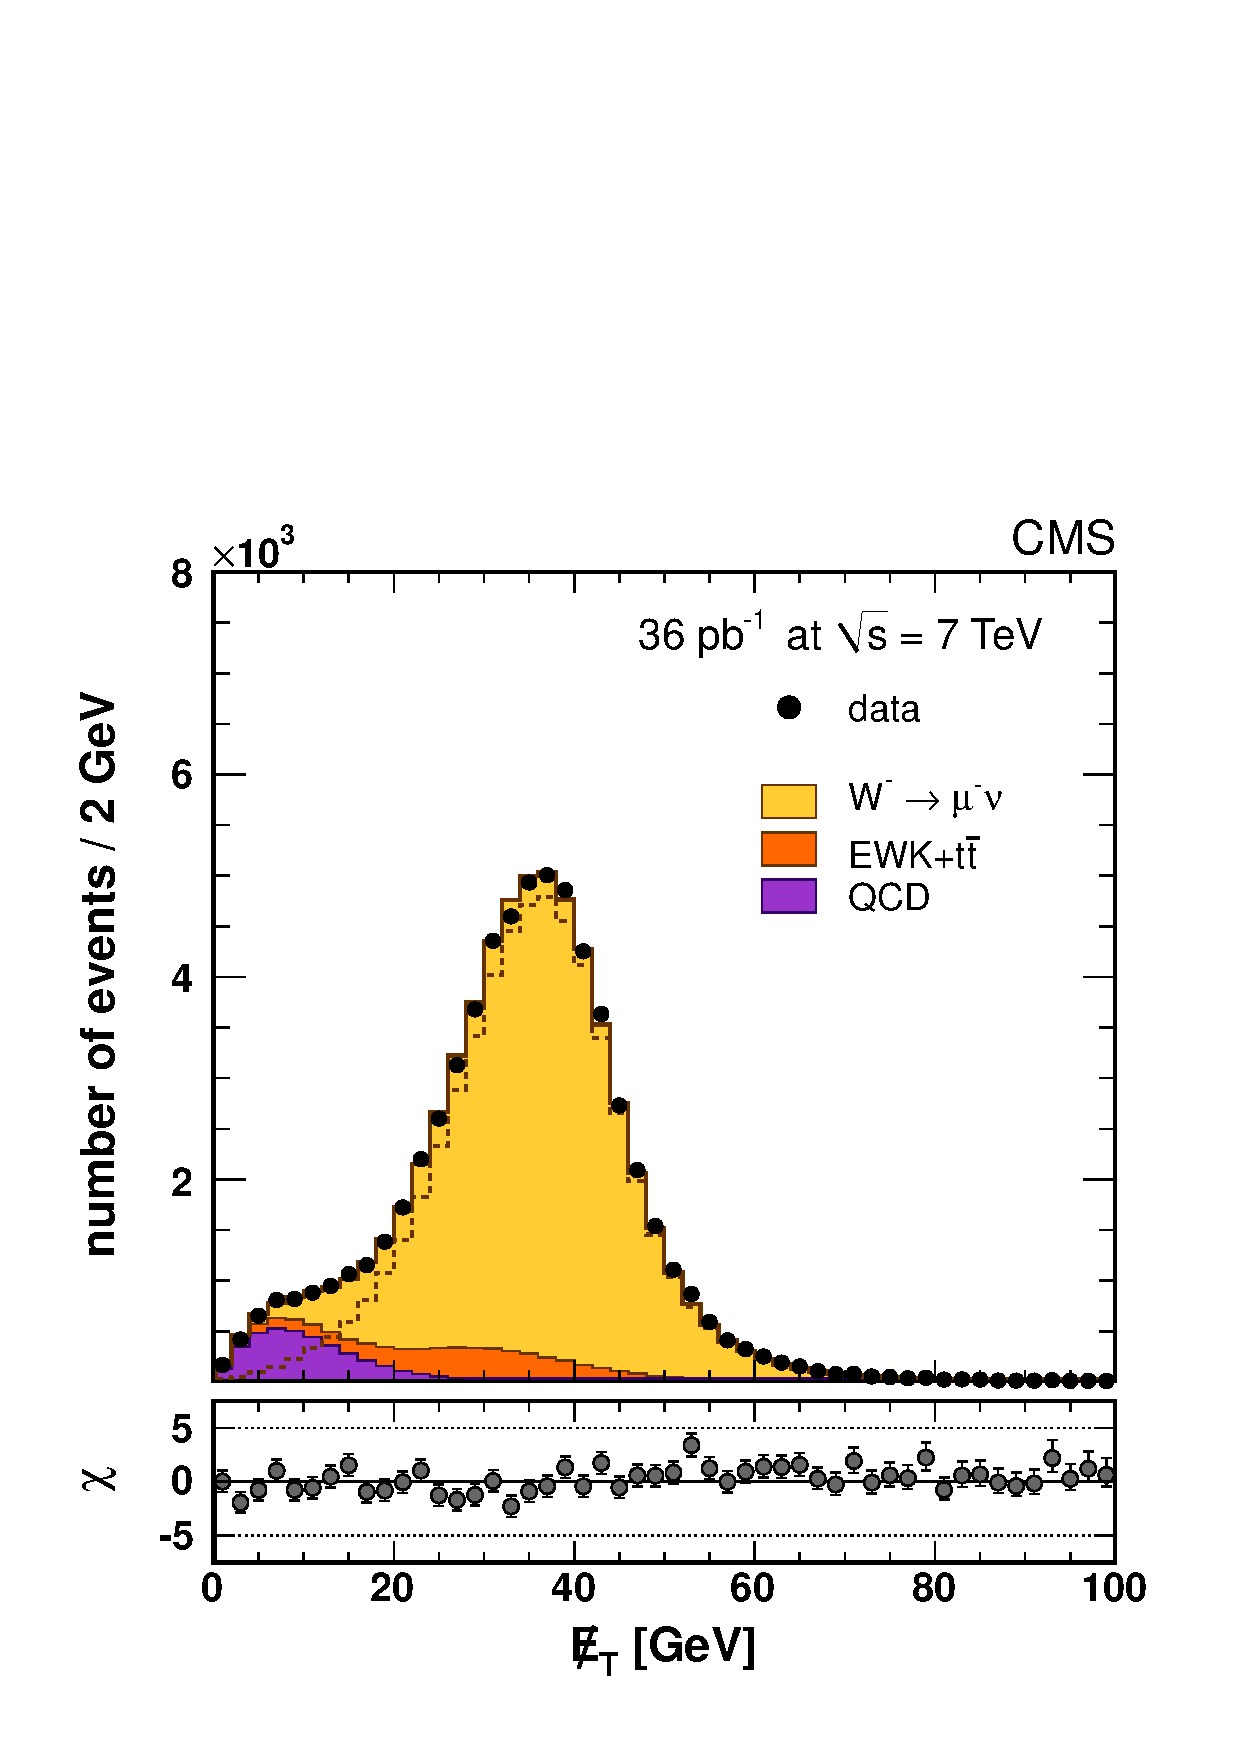
\includegraphics[width=7cm]{figs/Wmn_MET_minus.pdf}
    \caption{
The $\MET$ distributions for the selected W$^+$ (left) and W$^-$ (right) candidates.
The points with the error bars represent the data. Superimposed are the contributions
obtained with the fit for QCD background (violet, dark histogram), all other backgrounds
(orange, medium histogram), and signal plus background (yellow, light histogram).
The black dashed line is the fitted signal contribution.
    \label{figure:Wmn_PlusMinus}}
}
\end{figure}

 \begin{figure}[!ht] {\centering
   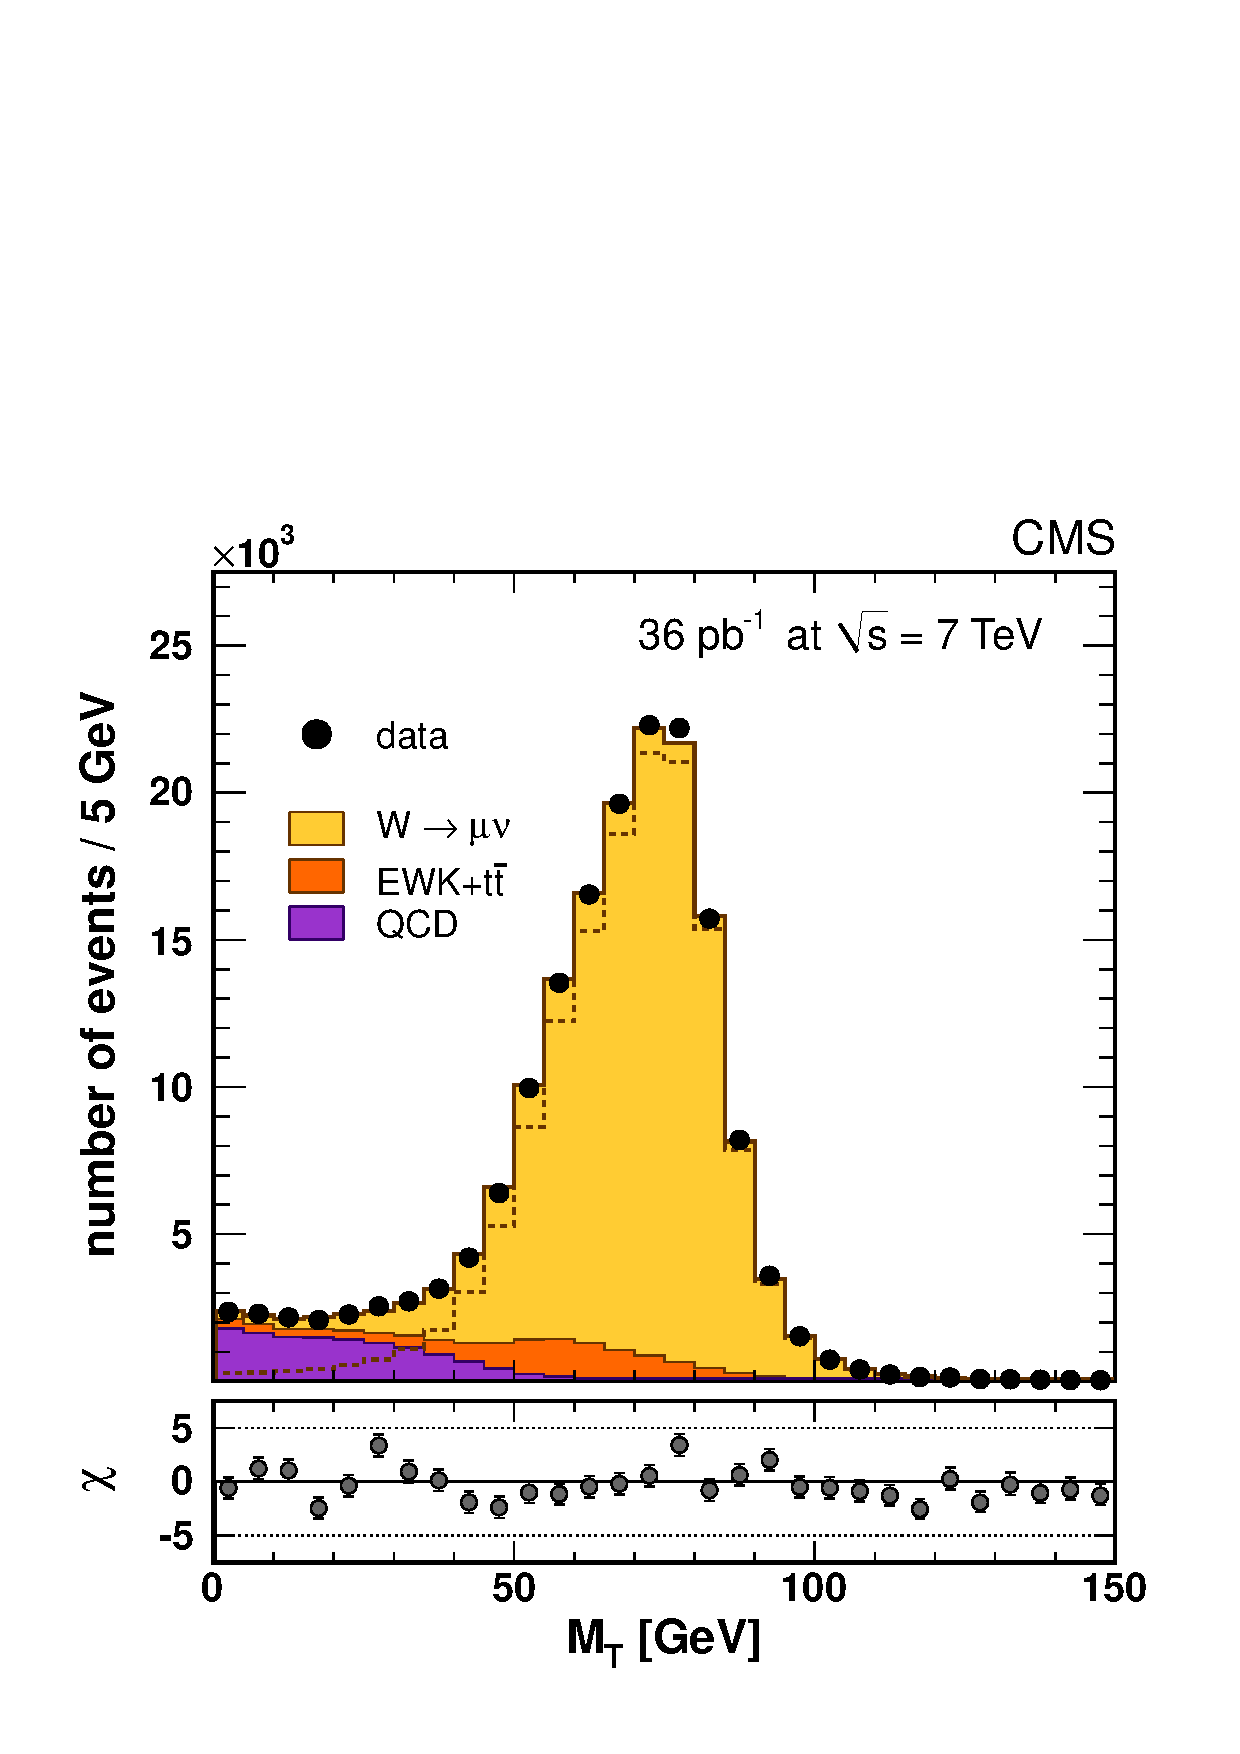
\includegraphics[width=7cm]{figs/Wmn_MT.pdf}
   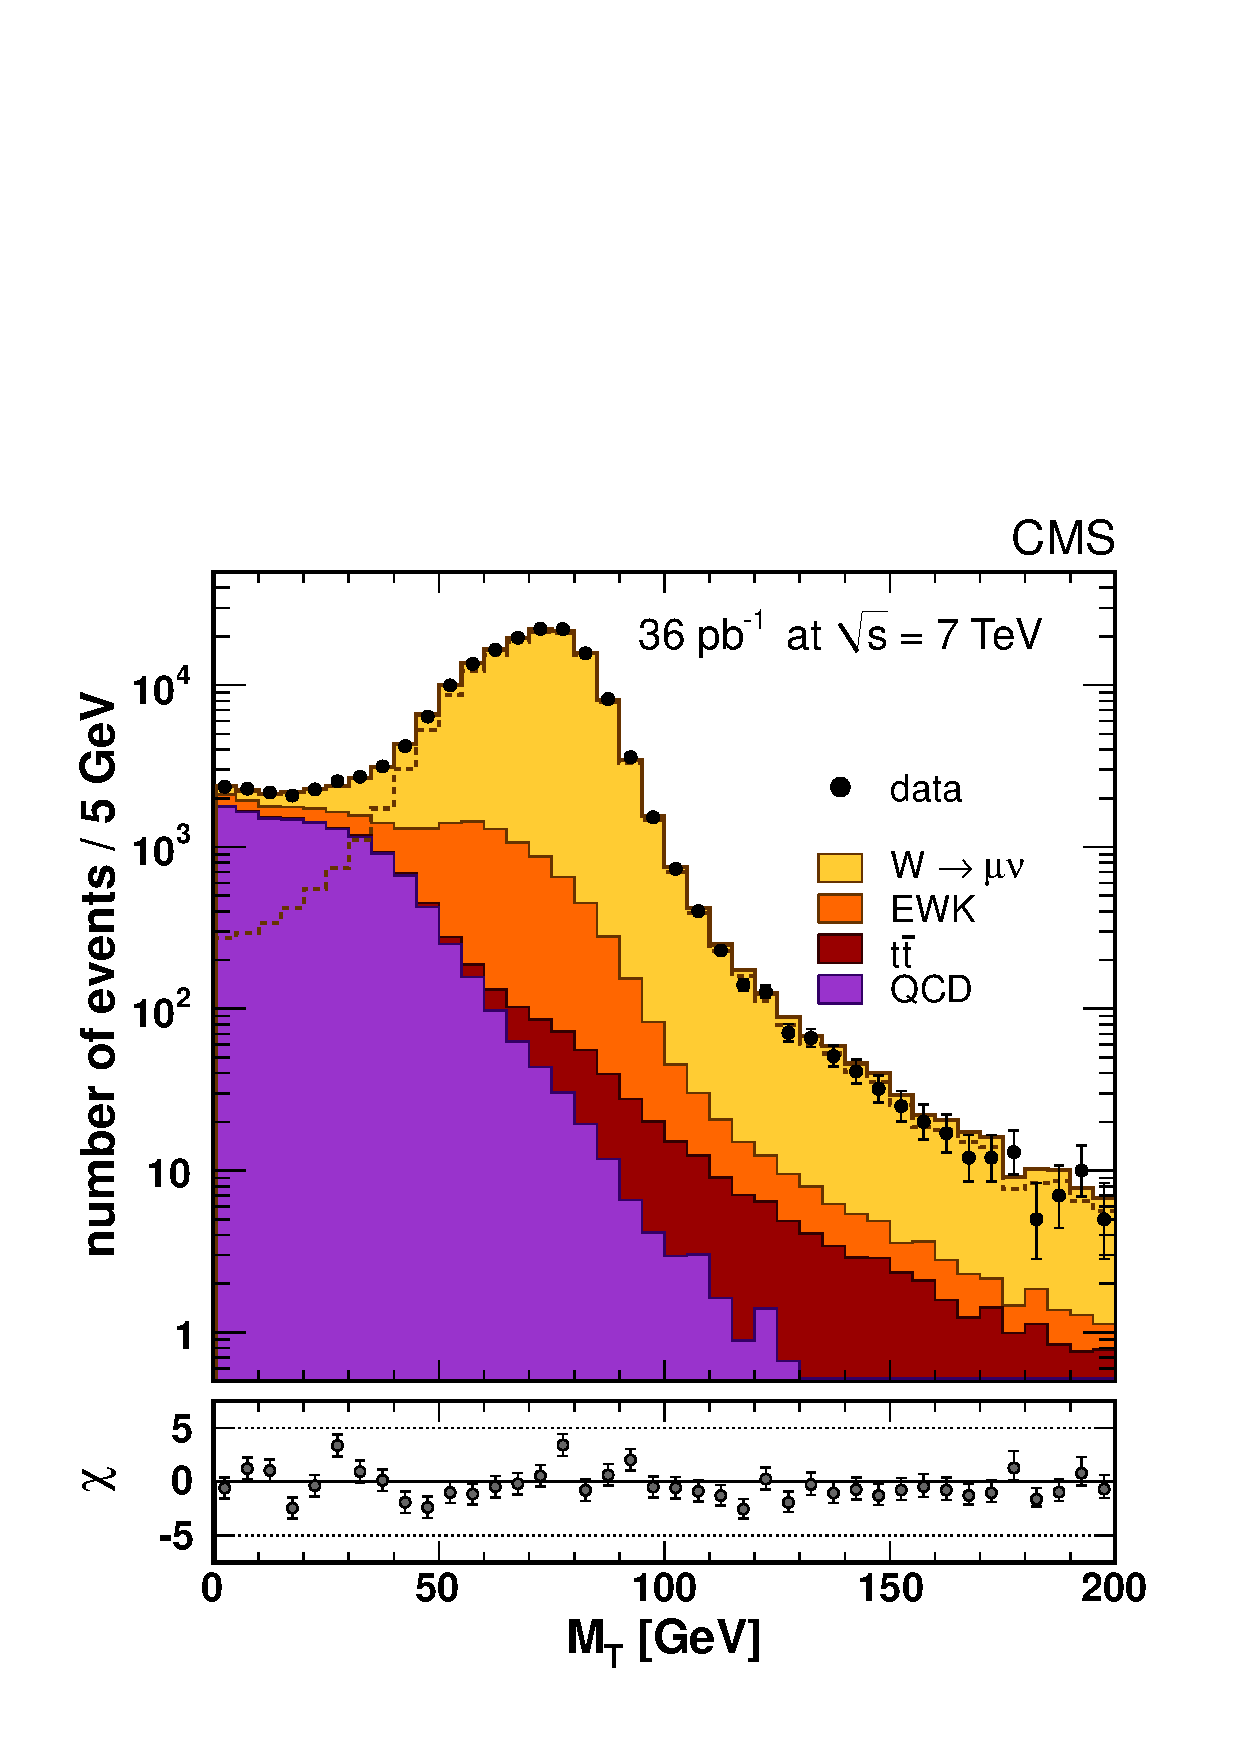
\includegraphics[width=7cm]{figs/Wmn_MT_log.pdf}
     \caption{
The $\MT$ distribution for the selected $\Wmn$ candidates on
a linear scale (left) and on a logarithmic scale (right).
The points with the error bars represent the data. Superimposed are the
contributions obtained with the fit
for QCD background (violet, dark histogram), all other backgrounds
(orange, medium histogram), and signal plus background (yellow, light histogram).
The black dashed line is the fitted signal contribution.
     \label{figure:Wmunu_exp_fit_mt}}
}
 \end{figure}



\section{\texorpdfstring{The $\Zll$ Signal Extraction}{The Z-> ll Signal Extraction}}
\label{sec:ZsignalExtraction}

The $\Zll$ yield can be obtained by counting the
number of selected candidates after subtracting the residual background.
The $\Zll$ yield and lepton efficiencies are also determined using a simultaneous fit
to the invariant mass spectra of multiple dilepton categories.
The simultaneous fit deals correctly with correlations
in determining the lepton efficiencies and the $\Zo$ yield
from the same sample.
The Z yield extracted in this way does not need to be corrected for efficiency effects
in order to determine the cross section, and
the statistical uncertainty on the $\Zo$ yield absorbs the uncertainties
on the determination of lepton efficiencies that would be propagated as systematic
uncertainties in the counting analysis.
Both methods were performed for the $\Zee$ analysis, while only
the simultaneous fit was used for the $\Zmm$ analysis
after taking into account the results from the previous studies~\cite{WZCMS:2010}.
%at lower luminosity which disfavour the use of the counting analysis.

\subsection{EWK and QCD Backgrounds}
\label{sec:bkgZll}

For the $\Zee$ analysis the background contributions from EWK processes $\Ztt$, $\ttbar$,
and diboson production are estimated from the yields of events selected in NLO MC samples
normalized to the NNLO cross sections and scaled to the considered integrated luminosity.
They amount to \ZEEEWKBKG events, where the uncertainty combines the NNLO
and luminosity uncertainties. Data are used to estimate the background
originating from W+jets, $\gamma$+jets, and QCD multijet events where the
selected electrons come from misidentified jets or photons
(referred to as 'QCD background').
This background contribution is estimated using the distribution
of the relative track isolation, $\ITRK/\Et$,
and amounts to $4.9 \pm 8.4\, \textrm{(stat.)} \pm 8.4\, \textrm{(syst.)}$ events.
As a cross-check, the ``same-sign/opposite-sign'' method was used,
which is based on the signs of the charges of the two electron candidates, the measured
charge misidentification for electrons that pass the nominal selection criteria, and the
hypothesis that the QCD background is charge-symmetric.
The QCD background estimate with this method is $59 \pm 17
\textrm{(stat.)} \pm 160\, \textrm{(syst.)}$ events.
The two methods are consistent with the presence of negligible QCD background in our sample.

Backgrounds in the $\Zmm$ analysis containing two isolated global muons
have been estimated with simulations to be very small.
This category of dimuon events is defined as the ``golden'' category.
The simulation prediction of the smallness of the $\ttbar$ and QCD backgrounds was validated with data.
First, the selected dimuon sample was enriched with $\ttbar$ events by applying
a requirement on $\MET$, because of the presence of neutrinos in $\ttbar$ events,
and an agreement between data and the simulation prediction was found
with the dimuon invariant mass requirement inverted,
where the residual Z signal is negligible.
The QCD component has been checked using the same-sign dimuon events and dimuon events with
both muons failing the isolation requirement, and was found to be in agreement with the simulation predictions.
The conclusion from the maximum amount of measured data-simulation discrepancy
was that the uncertainty in the residual background subtraction
has a negligible effect on the $\Zmm$ measured yield.
The backgrounds to the $\Zmm$ categories having one global and one looser muon
are significantly larger than in the golden category.
Simulation estimates in this case are not used for such backgrounds and
fits to the dimuon invariant mass
distributions are performed including parameterized background components, as
described in Section~\ref{sec:Zmumu}.

Backgrounds estimates in the $\Zee$ and $\Zmm$ analyses are summarized in Table~\ref{tab:ZllBG}.
%--------------------------------------------------
\begin{table} %
\begin{center}
\caption[.]{\label{tab:ZllBG}
Estimated background-to-signal ratios in the $\Zee$ and $\Zmm$ (only for candidates
in the golden category) channels.
The QCD background for the $\Zee$ channel has been estimated with data,
while all other estimates are based on MC simulations, and their corresponding uncertainties
are statistical only.}
\begin{tabular}{|l|c|c|}
\hline
Processes & $\Zee$ sel. & $\Zmm$ sel. \\
\hline\hline
Diboson production   & $(0.157\pm 0.001)\%$ & $(0.158\pm 0.001)\%$ \\
$\ttbar$             & $(0.117\pm 0.008)\%$ & $(0.141\pm 0.014)\%$ \\
$\Ztt$               & $(0.080\pm 0.006)\%$ & $(0.124\pm 0.005)\%$ \\
W+jets               & $(0.010\pm 0.002)\%$ & $(0.008\pm 0.002)\%$ \\
\hline
Total EWK plus $\ttbar$  & $(0.365\pm 0.010)\%$ & $(0.430\pm 0.015)\%$ \\
\hline
QCD            & $(0.06\pm 0.14)\%$ &  $(0.013\pm 0.001)\%$ \\
\hline
Total background                & $(0.42\pm 0.14)\%$ & $(0.444\pm 0.015)\%$ \\
\hline
\end{tabular}
\end{center}
\end{table}



%--------------------------------------------------


\subsection{\texorpdfstring{The $\Zee$ Signal Extraction}{The Z->ee Signal Extraction}}

In the following sections the use of a pure $\Zee$ sample
for the determination of the residual energy-scale and resolution corrections is first discussed.
Then the signal extraction with the counting analysis and the
simultaneous fit methods are presented.

\subsubsection{Electron Energy Scale}
\label{sec:e-escale}

The lead tungstate crystals of the ECAL are subject to transparency loss
during irradiation, followed by recovery in periods with no
irradiation. The magnitude of the changes to the energy response is
dependent on instantaneous luminosity and was, at the end of the 2010
data taking period, up to 1$\%$ in the barrel region, and 4$\%$ or more in
parts of the endcap. The changes are monitored continuously by injecting
laser light and recording the response. The corrections derived from
this monitoring are validated by studying the variation of the $\pi^0$ mass
peak as a function of time for different regions of the ECAL (using $\pi^0$ data
collected in a special calibration stream), and by studying the overall $\Zee$ mass peak and width.
%The correction
%calculations are still being developed and commissioned, and the
%corrections provided for the current reconstruction do not yet achieve
%the target precision. However, the validation and testing show that the
%residual variation of the energy scale with time, using these
%corrections, is less than 0.3$\%$ in the barrel and less than 1$\%$ in the
%endcap.
%
% from Isabel
%
With the current corrections, residual variations of the energy scale with time are
at the level of 0.3\% in the barrel and less than 1\% in the endcaps.


\par
%
% Isabel suggests to rewrite this section
%
%
The remaining mean scale correction factors to be applied to the data and the
resolution corrections (smearing) to be applied to the simulated sample
are estimated from $\Zee$ events. Invariant mass distributions for electrons
in several $\eta$ bins in the EB and EE are derived
from simulations and compared to data. A simultaneous fit of a Breit--Wigner convolved with a
Crystal-Ball function to each $\Zee$ mass distribution is performed  in order
to determine the energy scale correction factors for the data and the resolution
smearing corrections for the simulated samples. The energy scale correction
factors are below 1$\%$ while the resolution smearing corrections are below 1$\%$
everywhere, with the exception of the transition region between the EB and the EE,
where they reach 2$\%$.
Those corrections are propagated in the analysis and proper systematic uncertainties
for the cross section measurements are estimated as discussed in Section~\ref{subsec:ELEsystematics}.
%
%
% The remaining mean scale correction factors to be applied to the data and the
% resolution correction (smearing) to be applied to the simulated sample
% are estimated as follows.
% The $\Zee$ events are divided into categories that correspond to all possible
% combinations of four $\eta$ bins in the EB and two $\eta$ bins in the EE.
% An invariant mass distribution is derived from simulations in each category.
% A simultaneous fit of a Breit-Wigner convolved with a Crystal-Ball function
% to the $\Zee$ mass distribution is performed in each of the $\eta$ bins, in order
% to determine the energy scale correction factors for the data and the resolution
% smearing correction factors for the simulated samples.
% The energy scale correction factors for the data and the resolution smearing correction
% factors for the simulated samples for the tight selection are reported
% in Table~\ref{tab:EnergyScaleResolution}.
%
% \begin{table}[ht] %
%   \begin{center}
%   \caption{ Energy scale correction factors for the data and
% resolution smearing correction factors for the simulated samples
% to be applied per electron for various $\eta$ bins.
%   \label{tab:EnergyScaleResolution}}
%   \begin{tabular}{|l|c|c|}
%     \hline
%     Region  & Energy scale & Resolution Correction (smearing) [GeV] \\
%     \hline\hline
% $0.0<|\eta|<0.4$ & $0.9940\pm0.0010$ & $0.29\pm0.20$ \\
% $0.4<|\eta|<0.8$ & $0.9958\pm0.0011$ & $0.30\pm0.23$ \\
% $0.8<|\eta|<1.2$ & $0.9992\pm0.0012$ & $0.37\pm0.22$ \\
% $1.2<|\eta|<1.5$ & $1.0079\pm0.0020$ & $1.07\pm0.19$ \\
% $1.5<|\eta|<2.0$ & $0.9955\pm0.0019$ & $1.04\pm0.22$ \\
% $2.0<|\eta|<2.5$ & $1.0003\pm0.0013$ & $0.18\pm0.15$ \\
%     \hline
%     \end{tabular}
%   \end{center}
% \end{table}

\par
%
% This probably deserves to be put in a separate section instead of "Electron energy Scale"
% (Luca)
%
\subsubsection{Counting Analysis}
After energy scale corrections, applied to electron ECAL clusters before
any threshold requirement, 10 fewer events ($-0.12\%$) were selected compared to the number of selected
events before the application of the energy scale corrections.
This brings the final $\Zee$ sample to $\ZEESAMPLEN$ and, after
background subtraction, the $\Zo$ yield is $\ZEEYIELD$ events.
This yield is used for the cross section estimation.
%
% If this is not the result of the fit but just the counting
%


\par
The dielectron invariant mass spectra for the selected sample
with the tight selection before and after the application of the corrections are
shown in Fig.~\ref{fig:Zee} along with the predicted distributions.
The data and simulation distributions are normalized to account for the difference in selection
efficiency.

%%%%%
\begin{figure}
  \begin{center}
   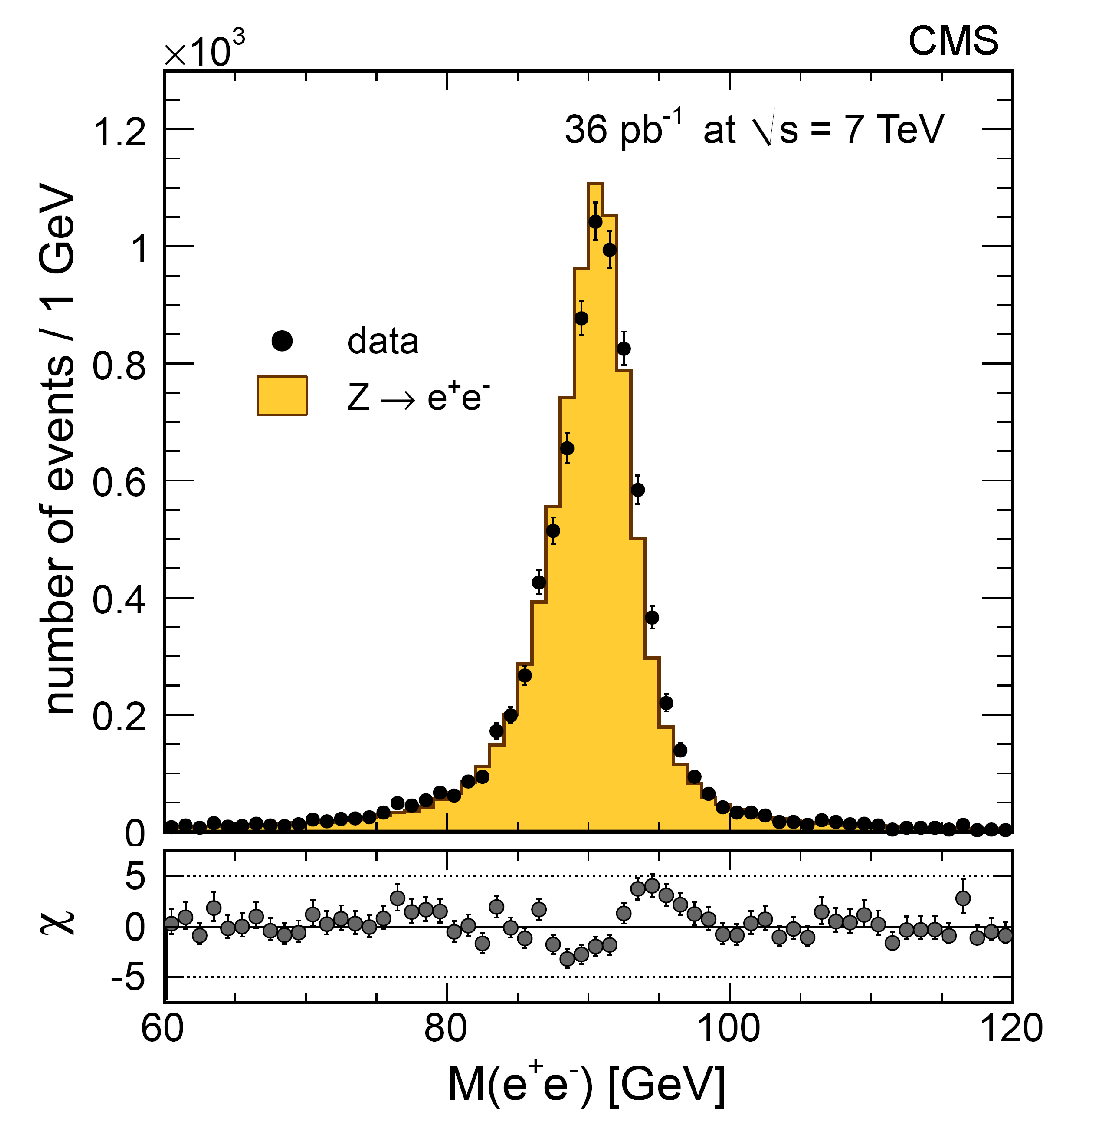
\includegraphics[width=0.48\textwidth]{figs/Zee_mass_Linear.pdf}
   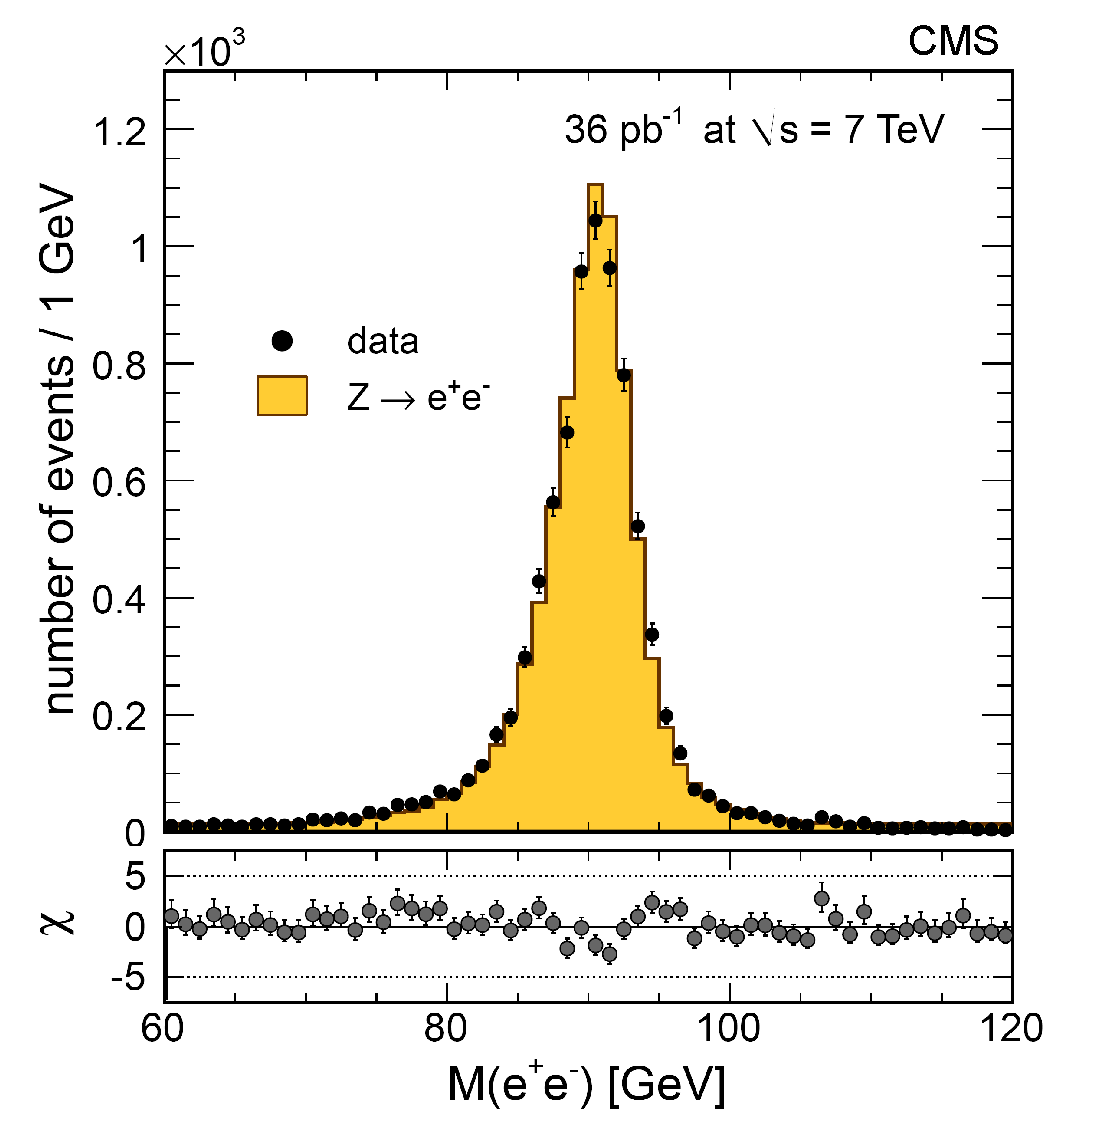
\includegraphics[width=0.48\textwidth]{figs/Zee_mass_Linear_corrected.pdf}
   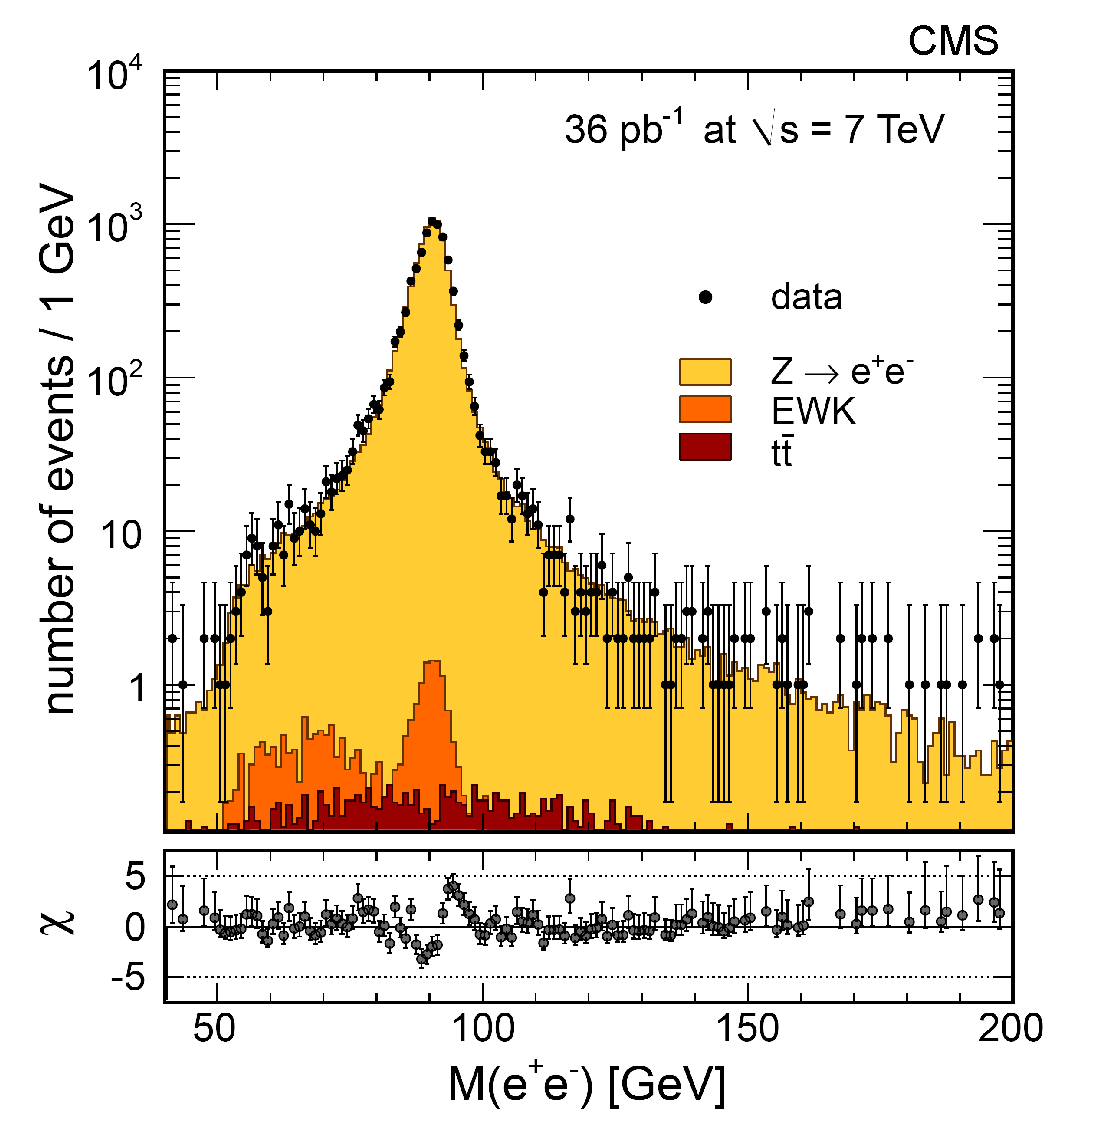
\includegraphics[width=0.48\textwidth]{figs/Zee_mass_Logarithmic.pdf}
   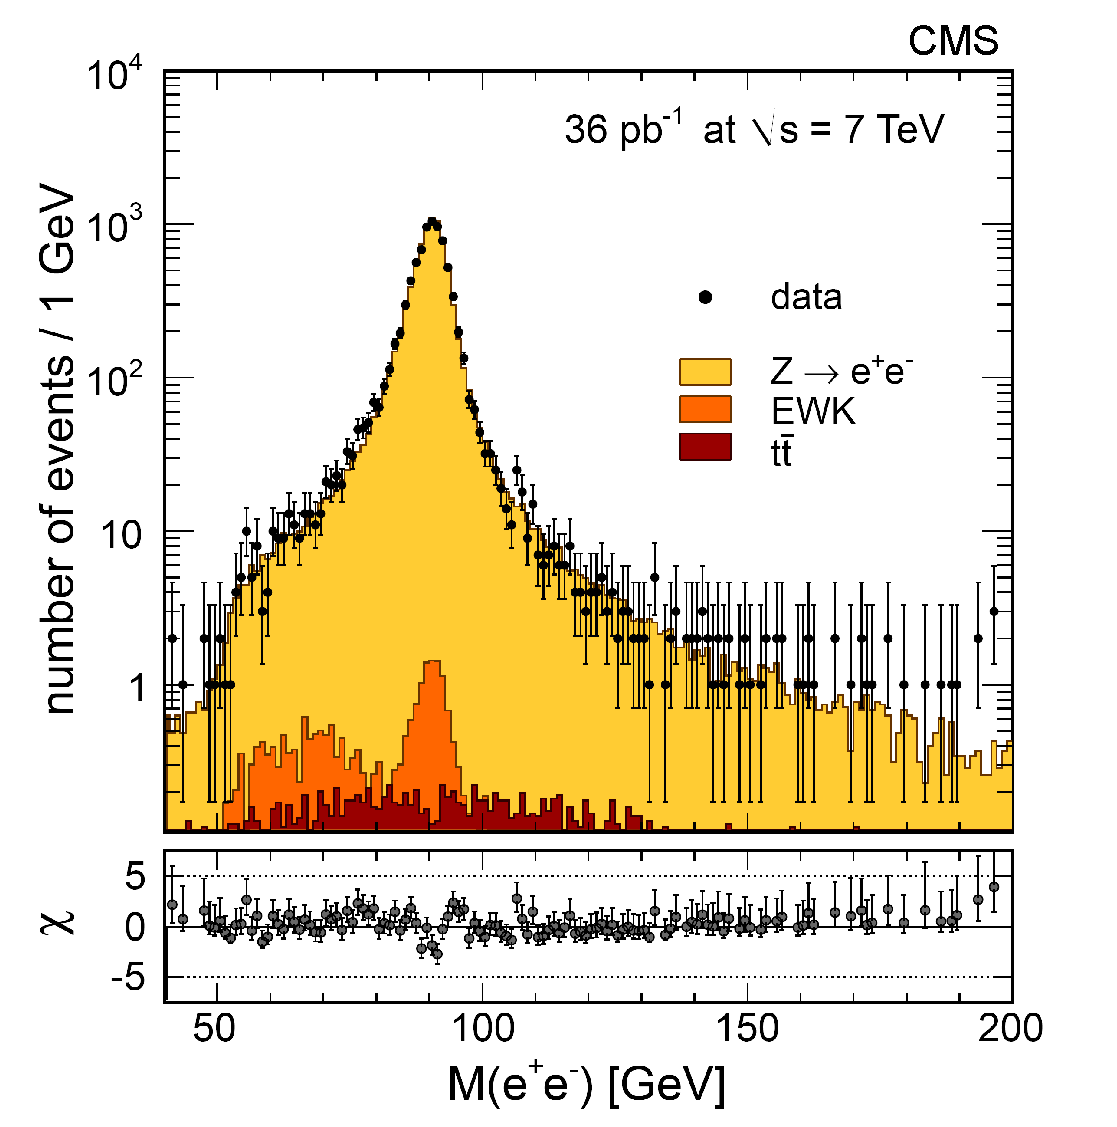
\includegraphics[width=0.48\textwidth]{figs/Zee_mass_Logarithmic_corrected.pdf}
   \caption{ \label{fig:Zee}
Distributions of the dielectron invariant mass for the selected $\Zee$ candidates on
a linear scale (top) and on a logarithmic scale (bottom) before (left)
and after (right) applying energy-scale correction factors.
The points with the error bars represent the data.
Superimposed are the expected distributions from simulations, normalized
to an integrated luminosity of $36$~pb$^{-1}$. The expected distributions are
the Z signal (yellow, light histogram), other EWK processes (orange, medium histogram),
and $\ttbar$ background (red, dark histogram).
Backgrounds are negligible and cannot be seen on the linear-scale plots.
}
  \end{center}
\end{figure}
%%%%%


\subsubsection{Simultaneous Fit}

The $\Zo$ event yield and the electron efficiencies can be extracted from
a simultaneous fit. Two categories of events are
considered: events where both electrons satisfy
the tight selection with $\Et>25\GeV$, and events that consist of
one electron with $\Et>25\GeV$ that passes the tight selection, and one
ECAL cluster with $\Et>25\GeV$ that fails
the selection, either at the reconstruction or electron identification level.

In each category, a signal-plus-background function is fitted to the observed mass spectrum.
The signal shape is taken from signal samples simulated with POWHEG at the NLO generator level,
and is convolved with a Crystal-Ball function modified to include an extra
Gaussian on the high end tail with floating mean and width.
In the first category, the nearly vanishing background is fixed to the
value reported in Table~\ref{tab:ZllBG}. In the second
category of events, the background is modeled by an exponential distribution.

%Fig.~\ref{fig:Zmass_TT_TF} shows the fit to the Tag-Tag events (left plot) and to
%Tag-Fail events (right plot).
The estimated cross section is $988 \pm 10\, \mathrm{(stat.)} \pm 4\mathrm{(syst.)}\,\mathrm{pb}$.
The cross section is in good agreement with the counting analysis estimate of
 $992 \pm 11\, \mathrm{(stat.)}\,\mathrm{pb}$, considering only the statistical uncertainty.
Both techniques give equivalent results. The counting analysis estimate is used for the
cross section measurement in the $\Zee$ channel.

%\begin{figure}
%  \begin{center}
%   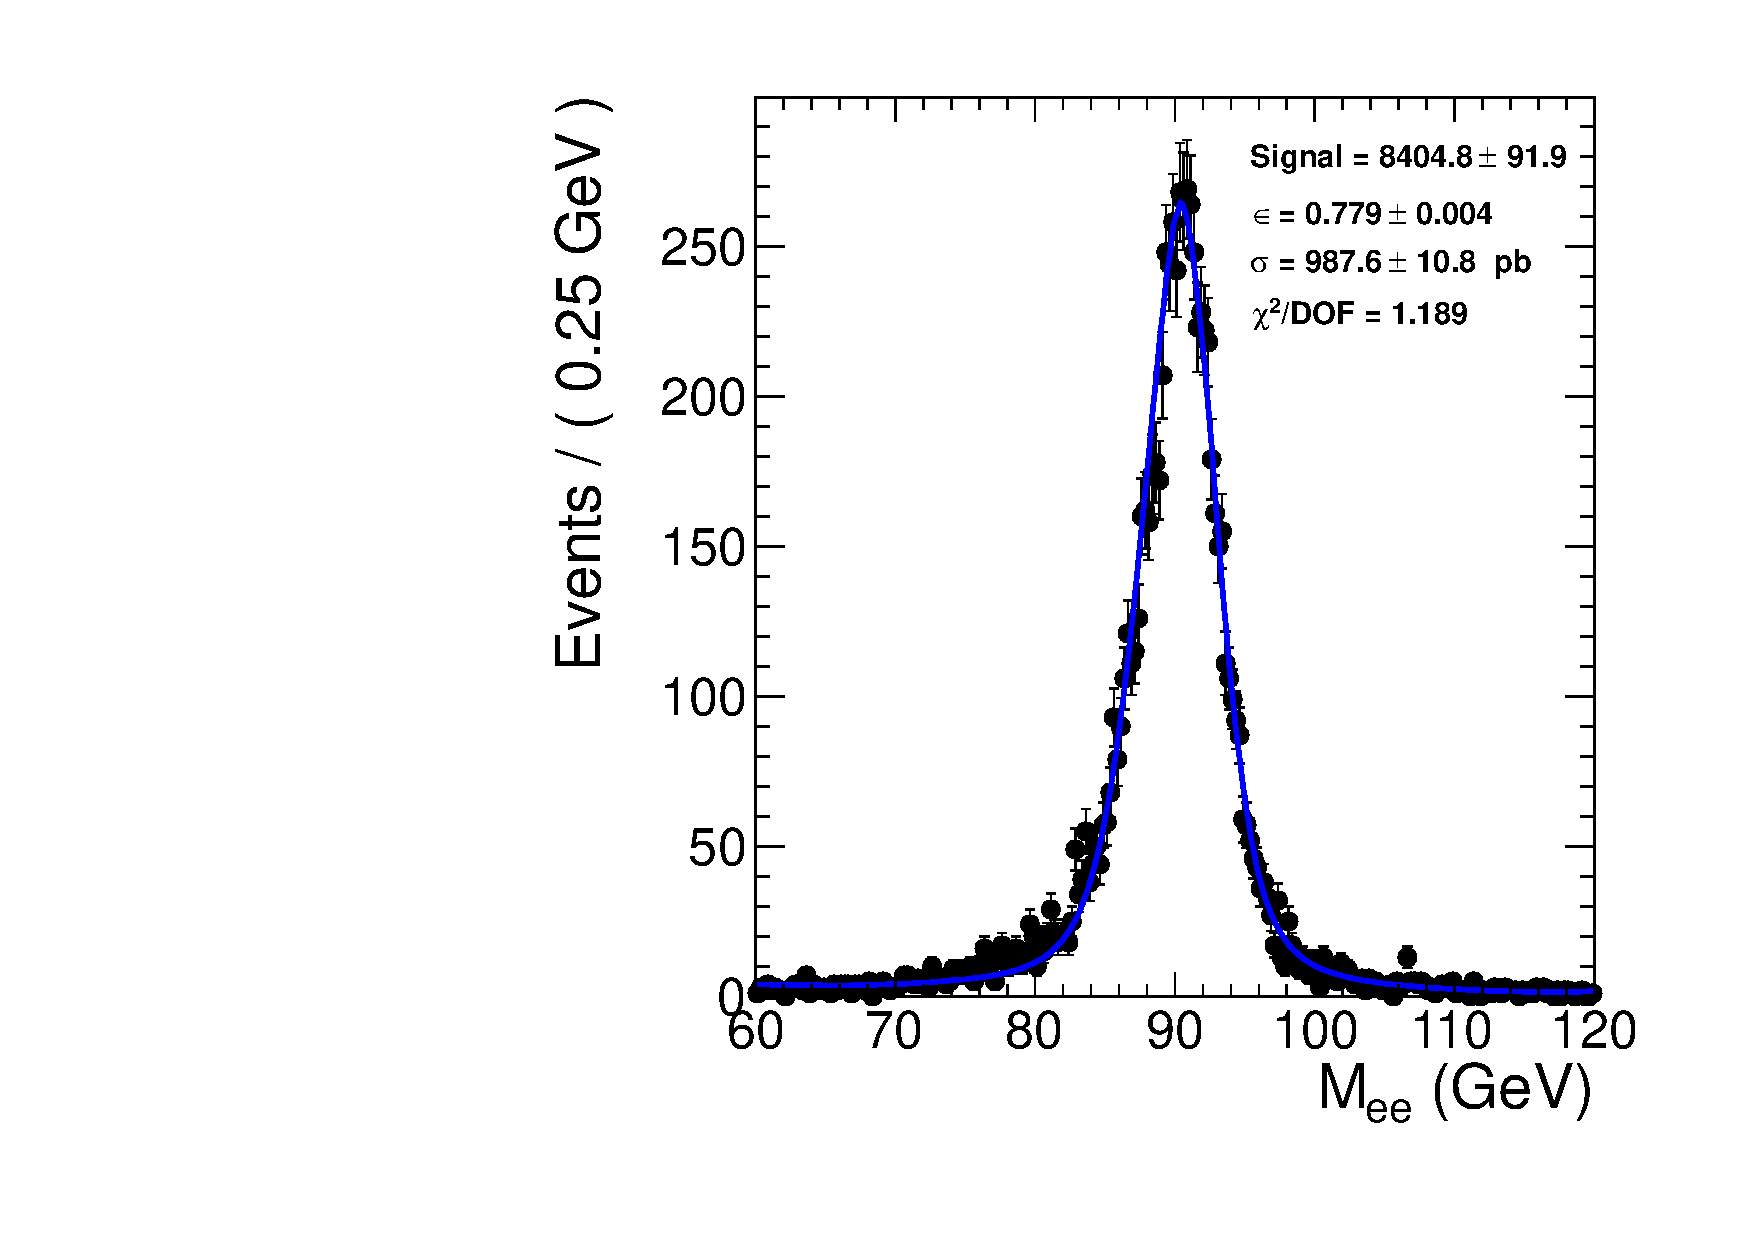
\includegraphics[width=0.48\textwidth]{figs/Zmass_TT_36143nb.pdf}
%   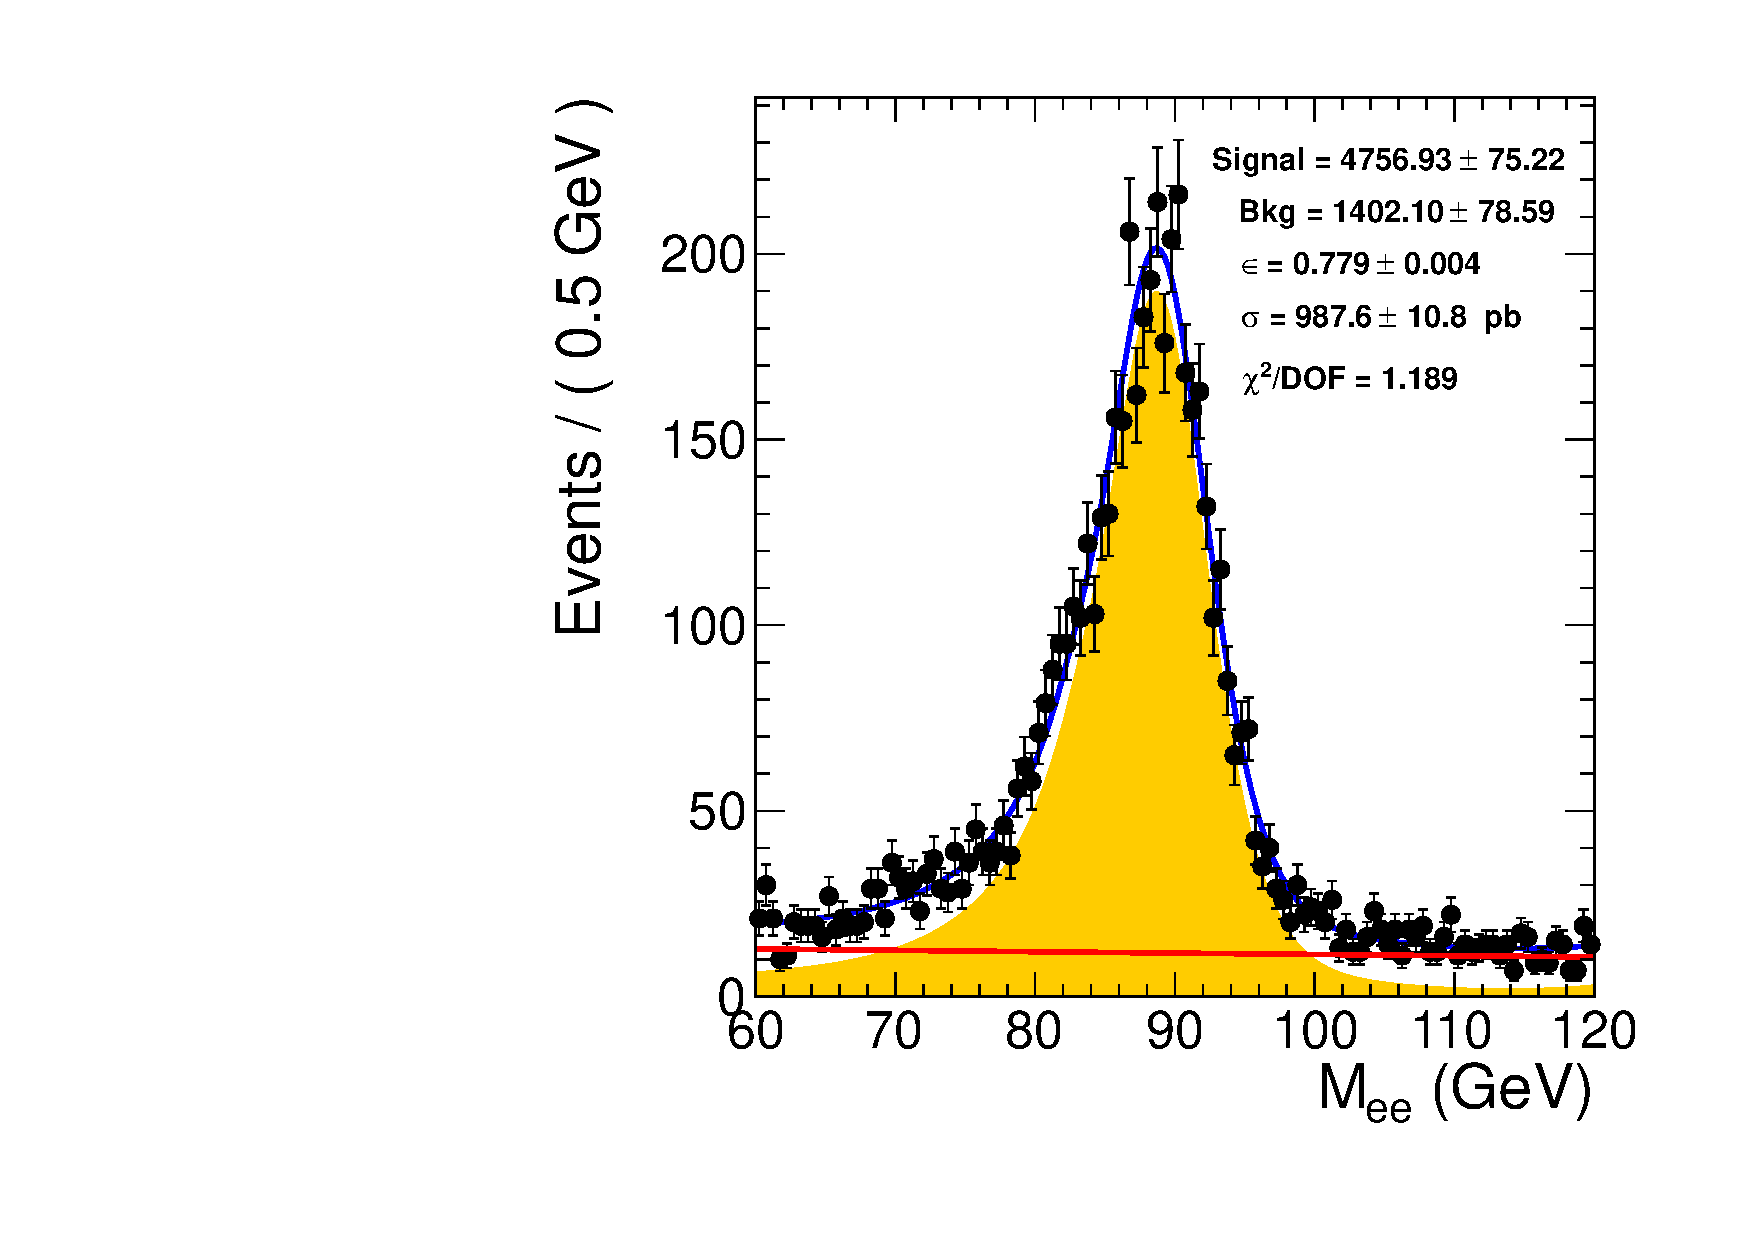
\includegraphics[width=0.48\textwidth]{figs/Zmass_TF_36143nb.pdf}
%   \caption{ \label{fig:Zmass_TT_TF}
%Fits to the Tag-Tag mass distributions (left plot) and Tag-Fail mass distributions (right plot)
%used in the simultaneous determination of the Zee yield and the electron efficiencies. }
%  \end{center}
%\end{figure}

%The electron $p_T$ distribution for $\Zee$ is shown in
%Fig.~\ref{fig:ZpT} in Appendix~\ref{sec:KinDist}.  Also,
%Fig.~\ref{fig:Zkin} shows the dielectron transverse
%momentum ($q_T$) and rapidity ($Y$) distributions.




\subsection{\texorpdfstring{The $\Zmm$ Signal Extraction}{The Z->mu mu Signal Extraction}}
\label{sec:Zmumu}

The yield of the $\Zmm$ events is determined from a fit simultaneously with the
average muon reconstruction efficiencies in the tracker and in
the muon detector, the muon trigger efficiency,
as well as the efficiency of the applied isolation requirement.
\Zmm candidates are obtained as pairs of muon candidates of different types
and organized into categories according to different requirements:
\begin{itemize}
\item $\Zmumu$: a pair of isolated global muons, further split into two samples:
\begin{itemize}
\item $\ZmumuTwoHlt$: each muons associated with an HLT trigger muon;
\item $\ZmumuOneHlt$: only one of the two muons associated with an HLT trigger muon;
\end{itemize}
\item $\Zmus$: one isolated global muon and one isolated
  stand-alone muon;
\item $\Zmut$: one isolated global muon and one isolated tracker track;
\item $\ZmumuNonIso$: a pair of global muons, of which one is isolated and the
other is nonisolated.
\end{itemize}

%The $\Zmumu$ category is also referred to as ``golden'' sample.
With the exception of the $\ZmumuOneHlt$ category, each global muon must correspond to an HLT trigger muon.
The five categories are explicitly forced to be mutually exclusive in the event
selection: if one event falls into the first category it is excluded from the second;
if it does not fall into the first category and falls into the second, it is excluded
from the third, and so on. In this way non-overlapping, hence statistically
independent, event samples are defined. The expected number of events in which more than
one dimuon combination is selected is almost negligible.
In those few cases all possible combinations are considered.

The five signal yields in each category can be written in terms of
the five unknowns, the Z signal yield $\NZtomumu$ and four efficiency terms, as follows:
\begin{eqnarray}
 \label{eqNmumuTwoHlt}
   \NmumuTwoHlt & = & \NZtomumu \effHlt^2 \effIso^2 \effTrk^2 \effSa^2,  \\
  \label{eqNmumuOneHlt}
   \NmumuOneHlt & = & 2 \NZtomumu \effHlt (1 - \effHlt) \effIso^2 \effTrk^2 \effSa^2,  \\
  \label{eqNmus}
   \Nmus & = & 2 \NZtomumu \effHlt \effIso^2 \effTrk (1 - \effTrk) \effSa^2,  \\
  \label{eqNmut}
   \Nmut & = & 2 \NZtomumu \effHlt \effIso^2 \effTrk^2 \effSa(1 -\effSa), \\
  \label{eqNmumuNonIso}
   \NmumuNonIso & = & 2 \NZtomumu \effHlt^2  \effIso (1 - \effIso)  \effTrk^2 \effSa^2.
\end{eqnarray}
The various efficiency terms in Eqs.~(\ref{eqNmumuTwoHlt}) to~(\ref{eqNmumuNonIso}),
the average efficiencies
of muon reconstruction in the tracker, $\effTrk$, in the muon detector as
a stand-alone muon, $\effSa$, the average efficiency of the isolation requirement,
$\effIso$, and the average trigger efficiency, $\effHlt$,
can be factorized because the muon selection
factorizes the requirements on the tracker and muon detector quantities separately.
Neither selection on $\chi^2$ per degree of freedom nor requirement of the muon reconstruction through the
tracker-muon algorithm is applied in order to
avoid efficiency terms that cannot be described as a product of contributions from the tracker and
the muon detector.
%We verified on Monte Carlo that the possible effects of any residual correlation
%can be either incorporated in the proper definition of the efficiencies or
%is negligible.
% Above, $\effTrk$ is
% the efficiency to reconstruct a track {\it and} to pass the track selection,
% and $\effSa$ is the efficiency to reconstruct a track in the muon detector {\it and} to pass the
% stand-alone muon selection, according to the selection described in Section~\ref{sec:muonid}.

The dimuon invariant mass spectra for the five categories are divided into
bins of different sizes, depending on the number of observed events.
The distributions of the dimuon invariant mass for the different categories can be written
as the sum of a signal peak plus a background component.


Figure~\ref{fig:zGolden36pb} shows the dimuon invariant mass spectrum for the $\Zmm$ golden events
on both a linear scale and a logarithmic scale, and Figs.~\ref{fig:zNoGold1}
and~\ref{fig:zNoGold2} show the
invariant mass distributions for the remaining categories.
The spectra are in agreement with the simulation.

\begin{figure}[hbtp]
    \begin{minipage}{73mm}
      \begin{center}
%        \resizebox{1.0\textwidth}{!}{{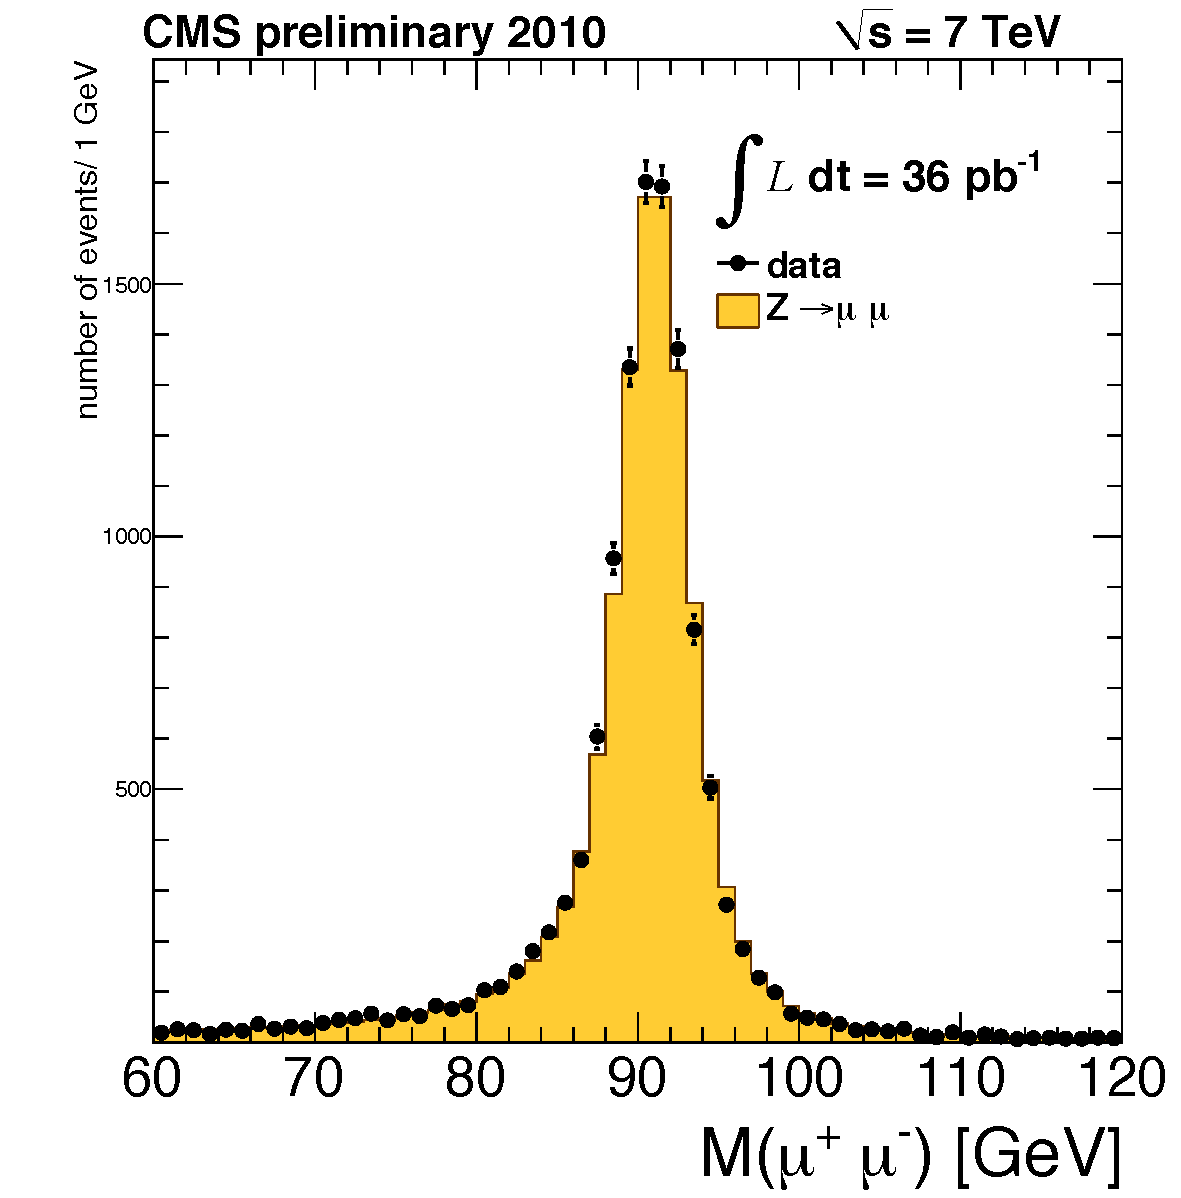
\includegraphics{figs/zGoldenLin_36pb.pdf}}}
        \resizebox{1.0\textwidth}{!}{{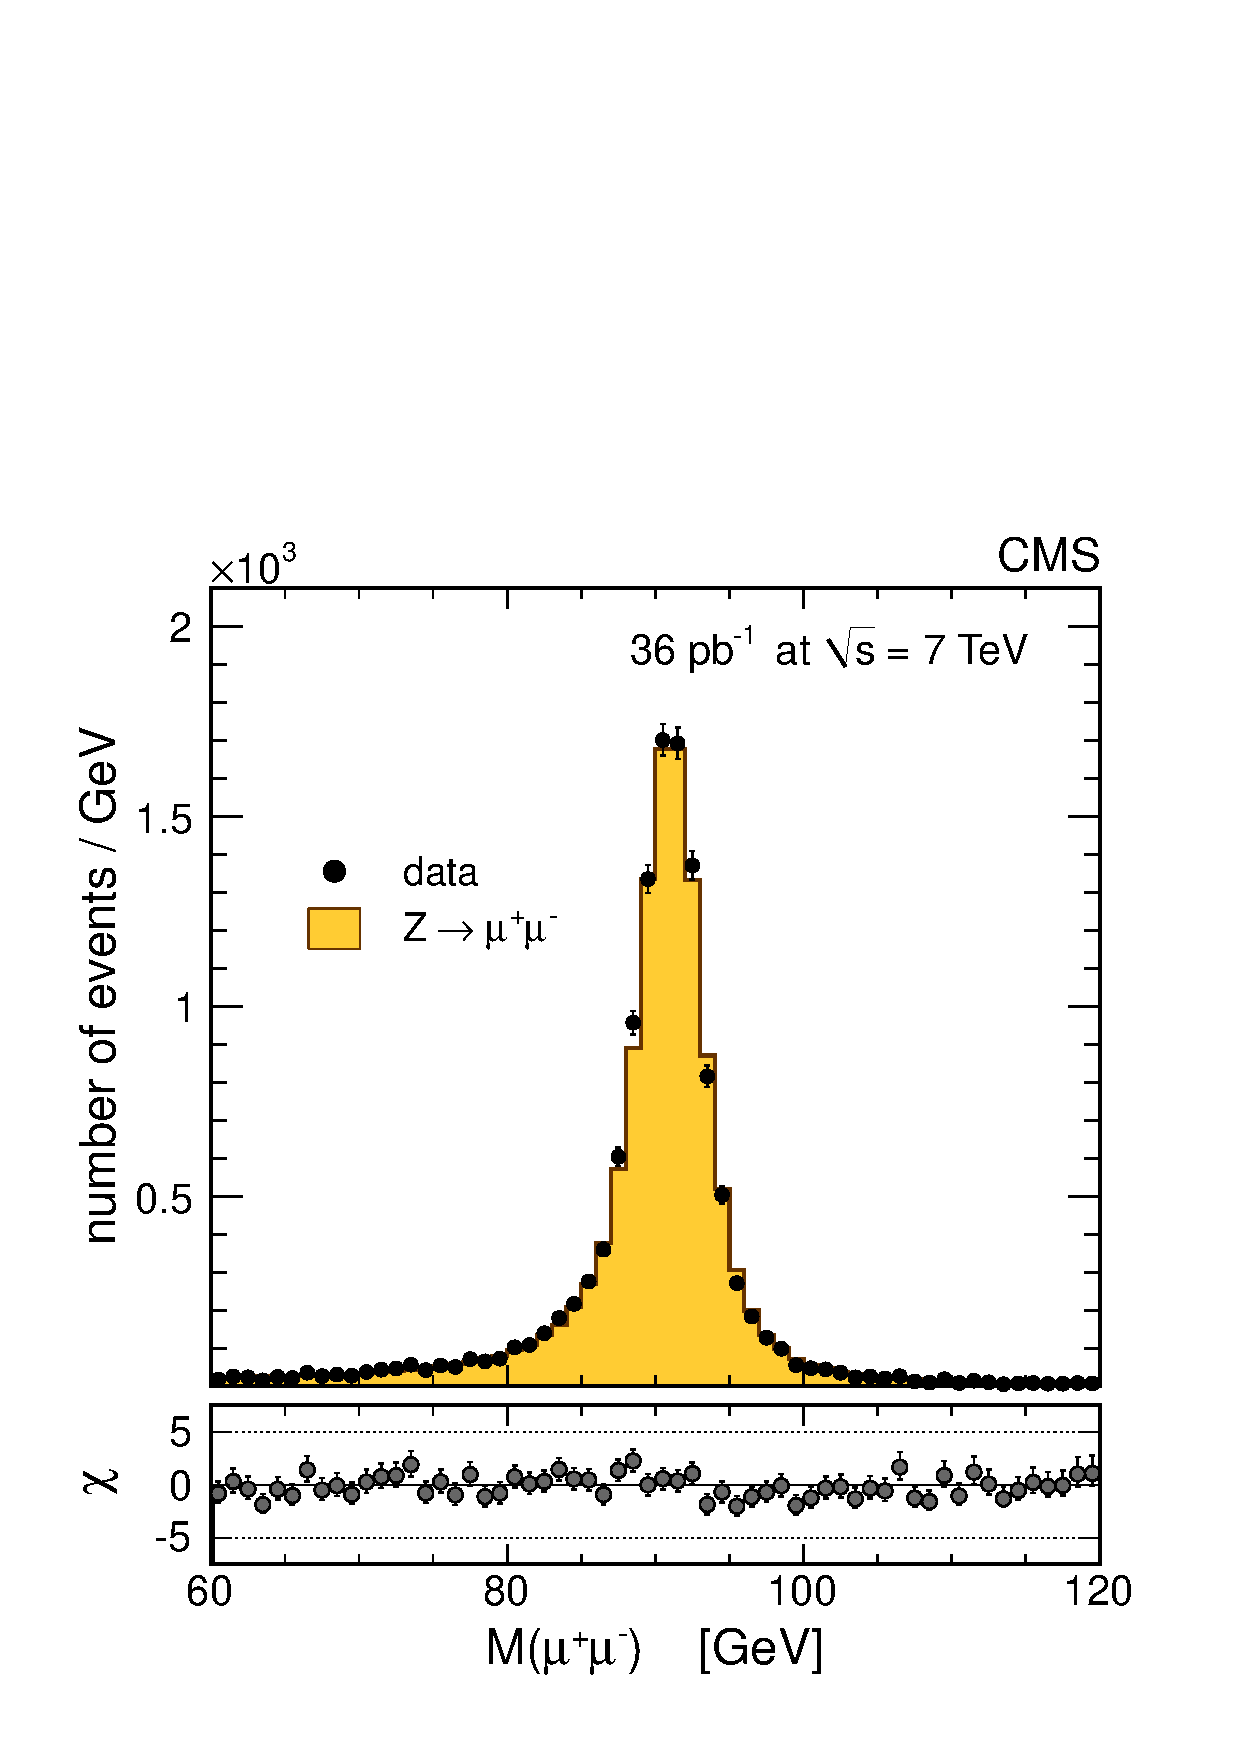
\includegraphics{figs/Zmumu_lin.pdf}}}
      \end{center}
    \end{minipage}
    \begin{minipage}{73mm}
       \begin{center}
%       \resizebox{!}{1.0\textwidth}{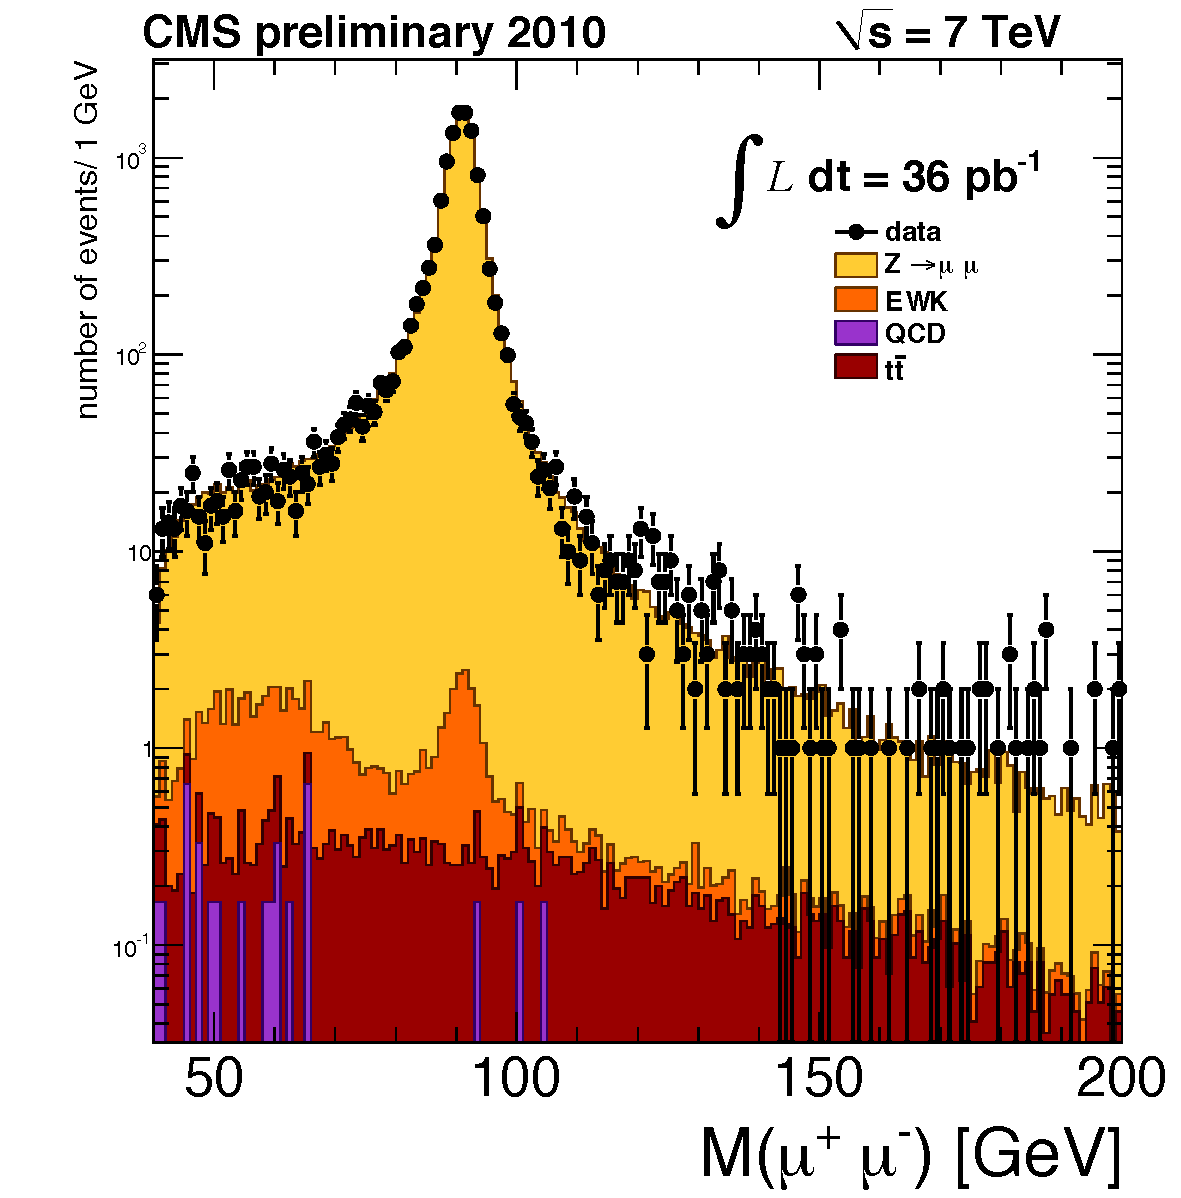
\includegraphics{figs/zGoldenLog_36pb.pdf}}
       \resizebox{!}{1.0\textwidth}{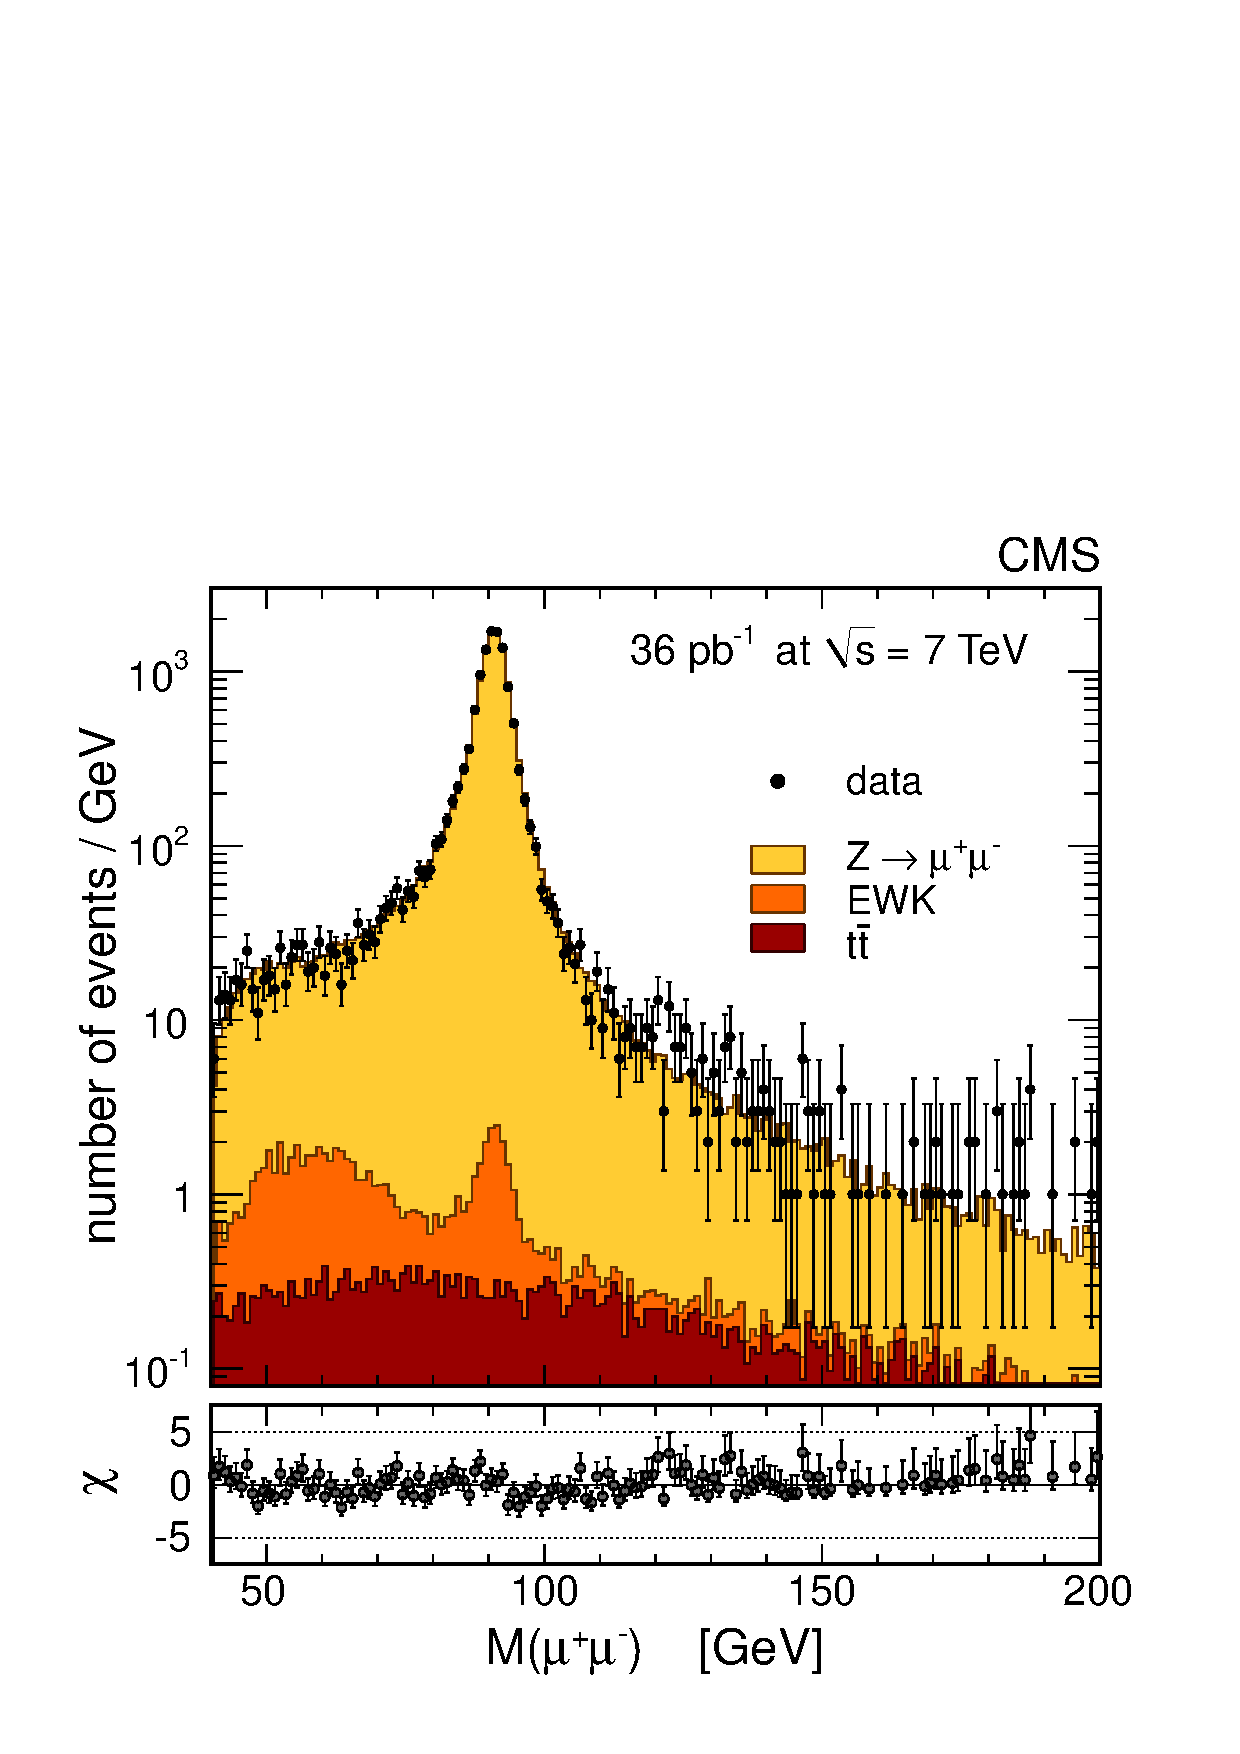
\includegraphics{figs/Zmumu_log.pdf}}
      \end{center}
    \end{minipage}
\caption{
Distributions of the dimuon invariant mass for the selected $\Zmm$ golden candidates on
a linear scale (left) and on a logarithmic scale (right).
The points with the error bars represent the data.
Superimposed are the expected distributions from simulations, normalized
to an integrated luminosity of $36$~pb$^{-1}$. The expected distributions are
the Z signal (yellow, light histogram), other EWK processes (orange, medium histogram),
and $\ttbar$ background (red, dark histogram).
Backgrounds are negligible and cannot be seen on the linear-scale plots.
}
\label{fig:zGolden36pb}
\end{figure}

\begin{figure}[hbtp]
    \begin{minipage}{73mm}
      \begin{center}
        \resizebox{1.0\textwidth}{!}{{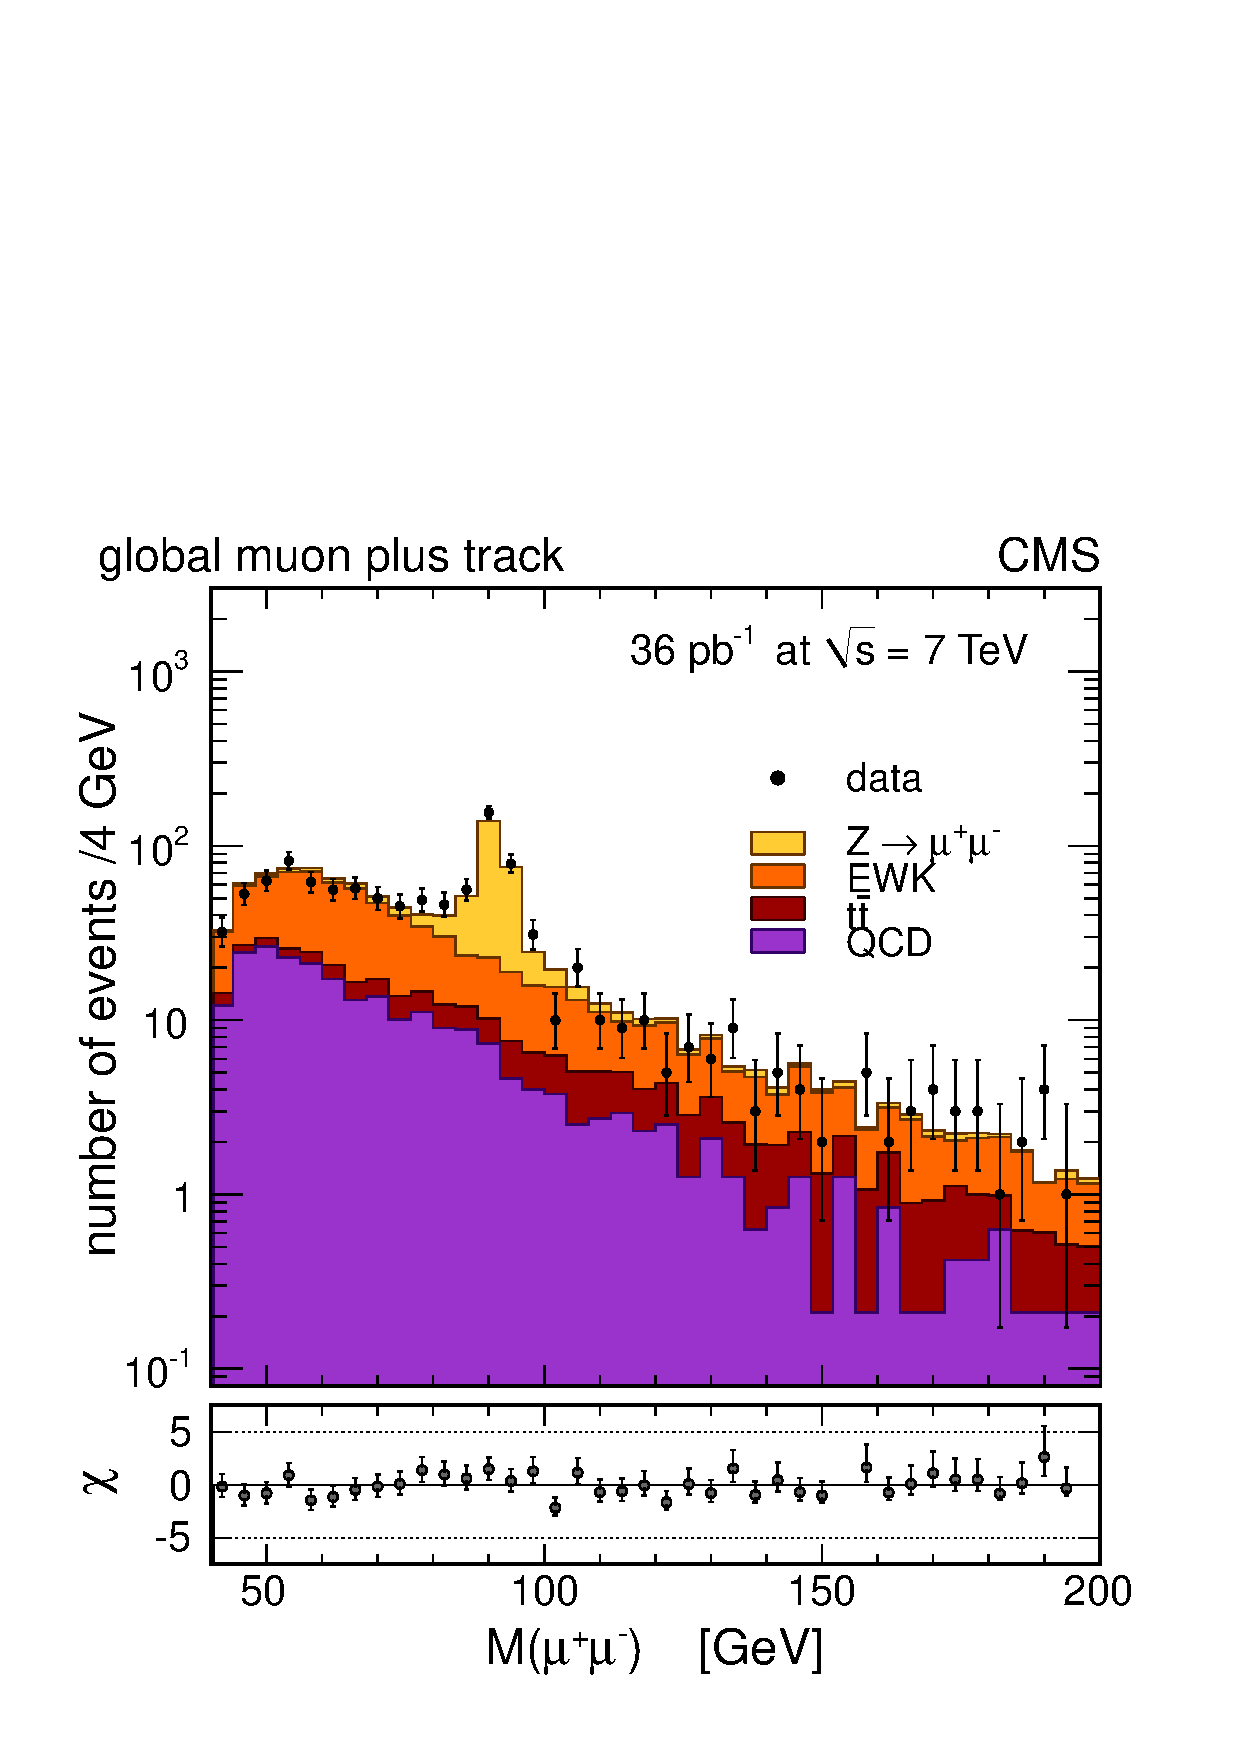
\includegraphics{figs/ZMuTrk_log.pdf}}}
      \end{center}
    \end{minipage}
    \begin{minipage}{73mm}
       \begin{center}
       \resizebox{!}{1.0\textwidth}{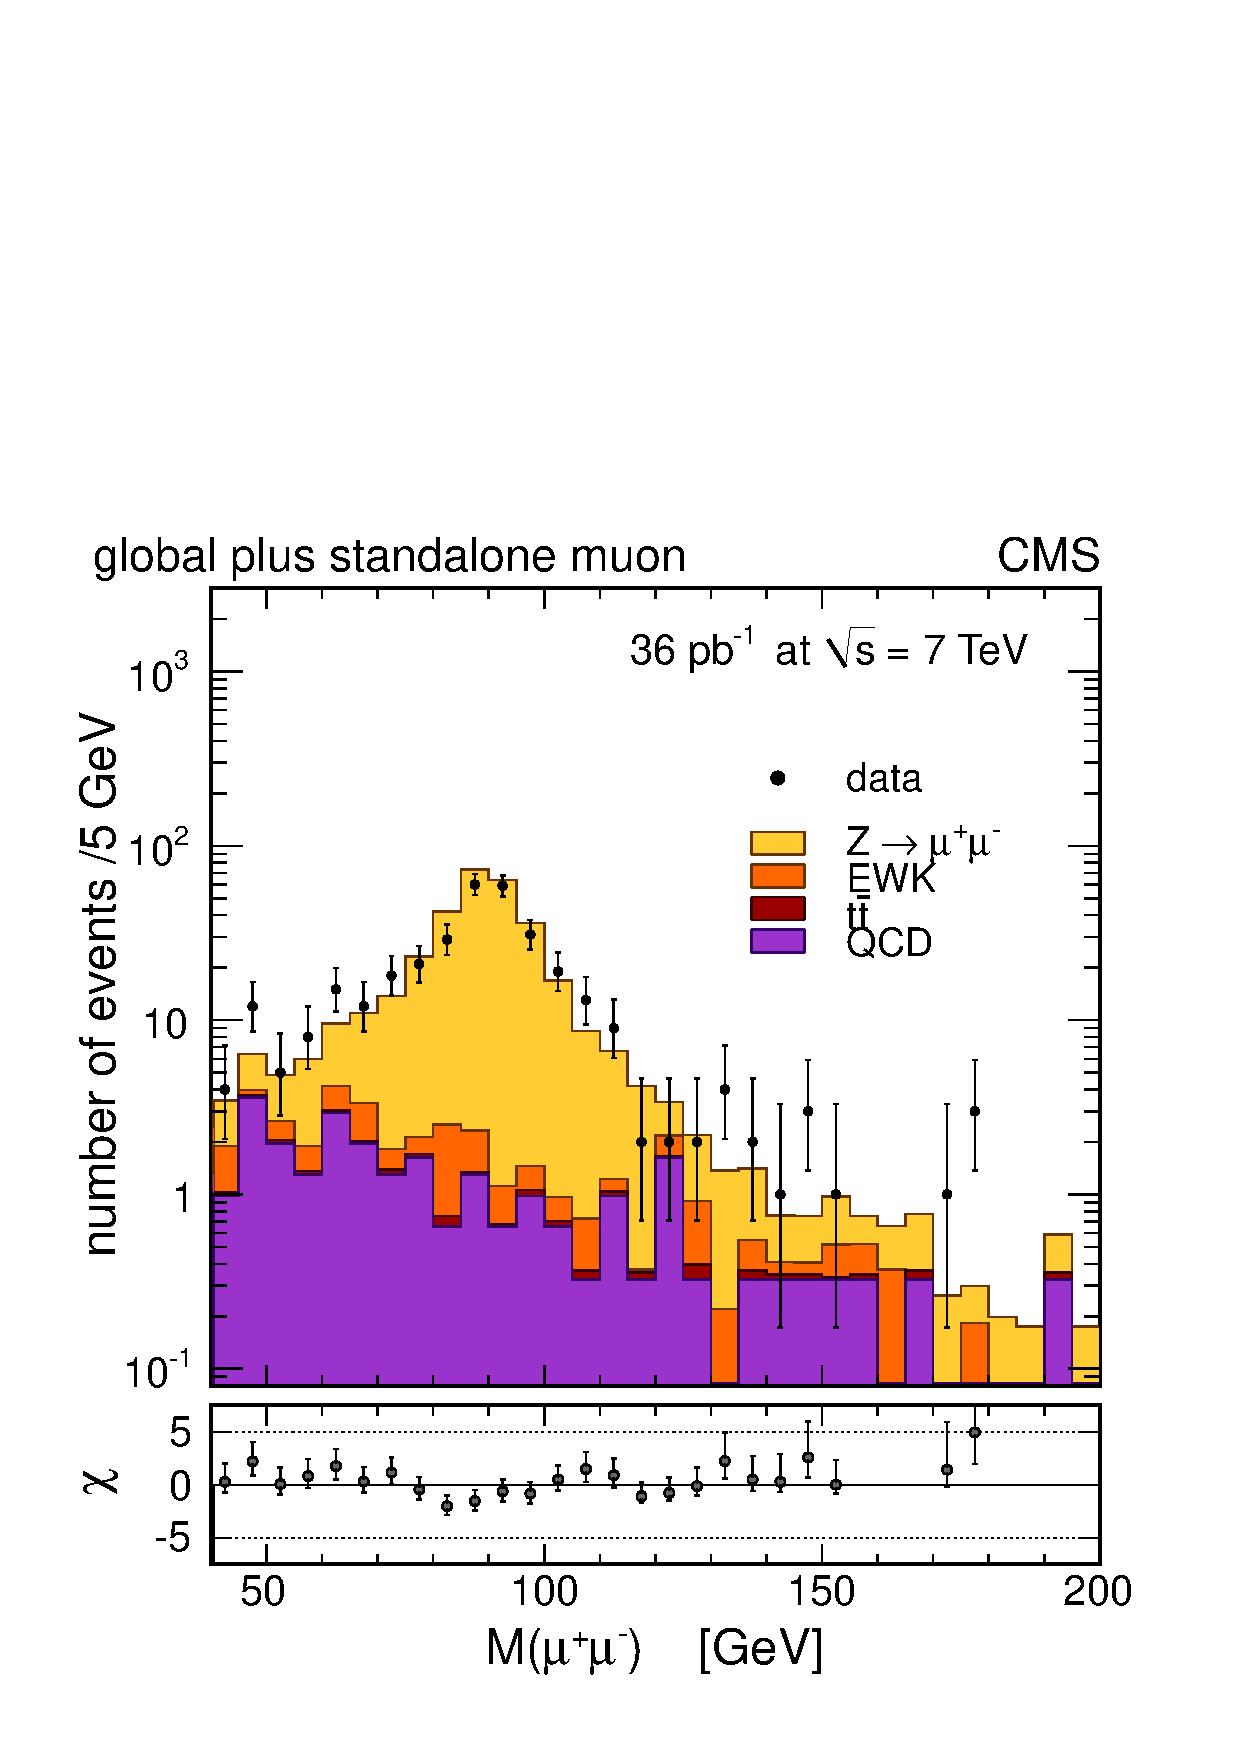
\includegraphics{figs/ZMuSta_log.pdf}}
      \end{center}
    \end{minipage}
\caption{Distributions of the dimuon invariant mass for the selected
$\Zmut$ (left) and $\Zmus$ (right) candidates.
The points with the error bars represent the data.
Superimposed are the expected distributions from simulations, normalized
to an integrated luminosity of $36$~pb$^{-1}$. The expected distributions are
the Z signal (yellow, light histogram), other EWK processes (orange, medium histogram),
$\ttbar$ background (red, dark histogram) and QCD background (violet, black histogram).
}
\label{fig:zNoGold1}
\end{figure}
\begin{figure}[hbtp]
    \begin{center}
     \begin{minipage}{73mm}
       \begin{center}
        \resizebox{!}{1.0\textwidth}{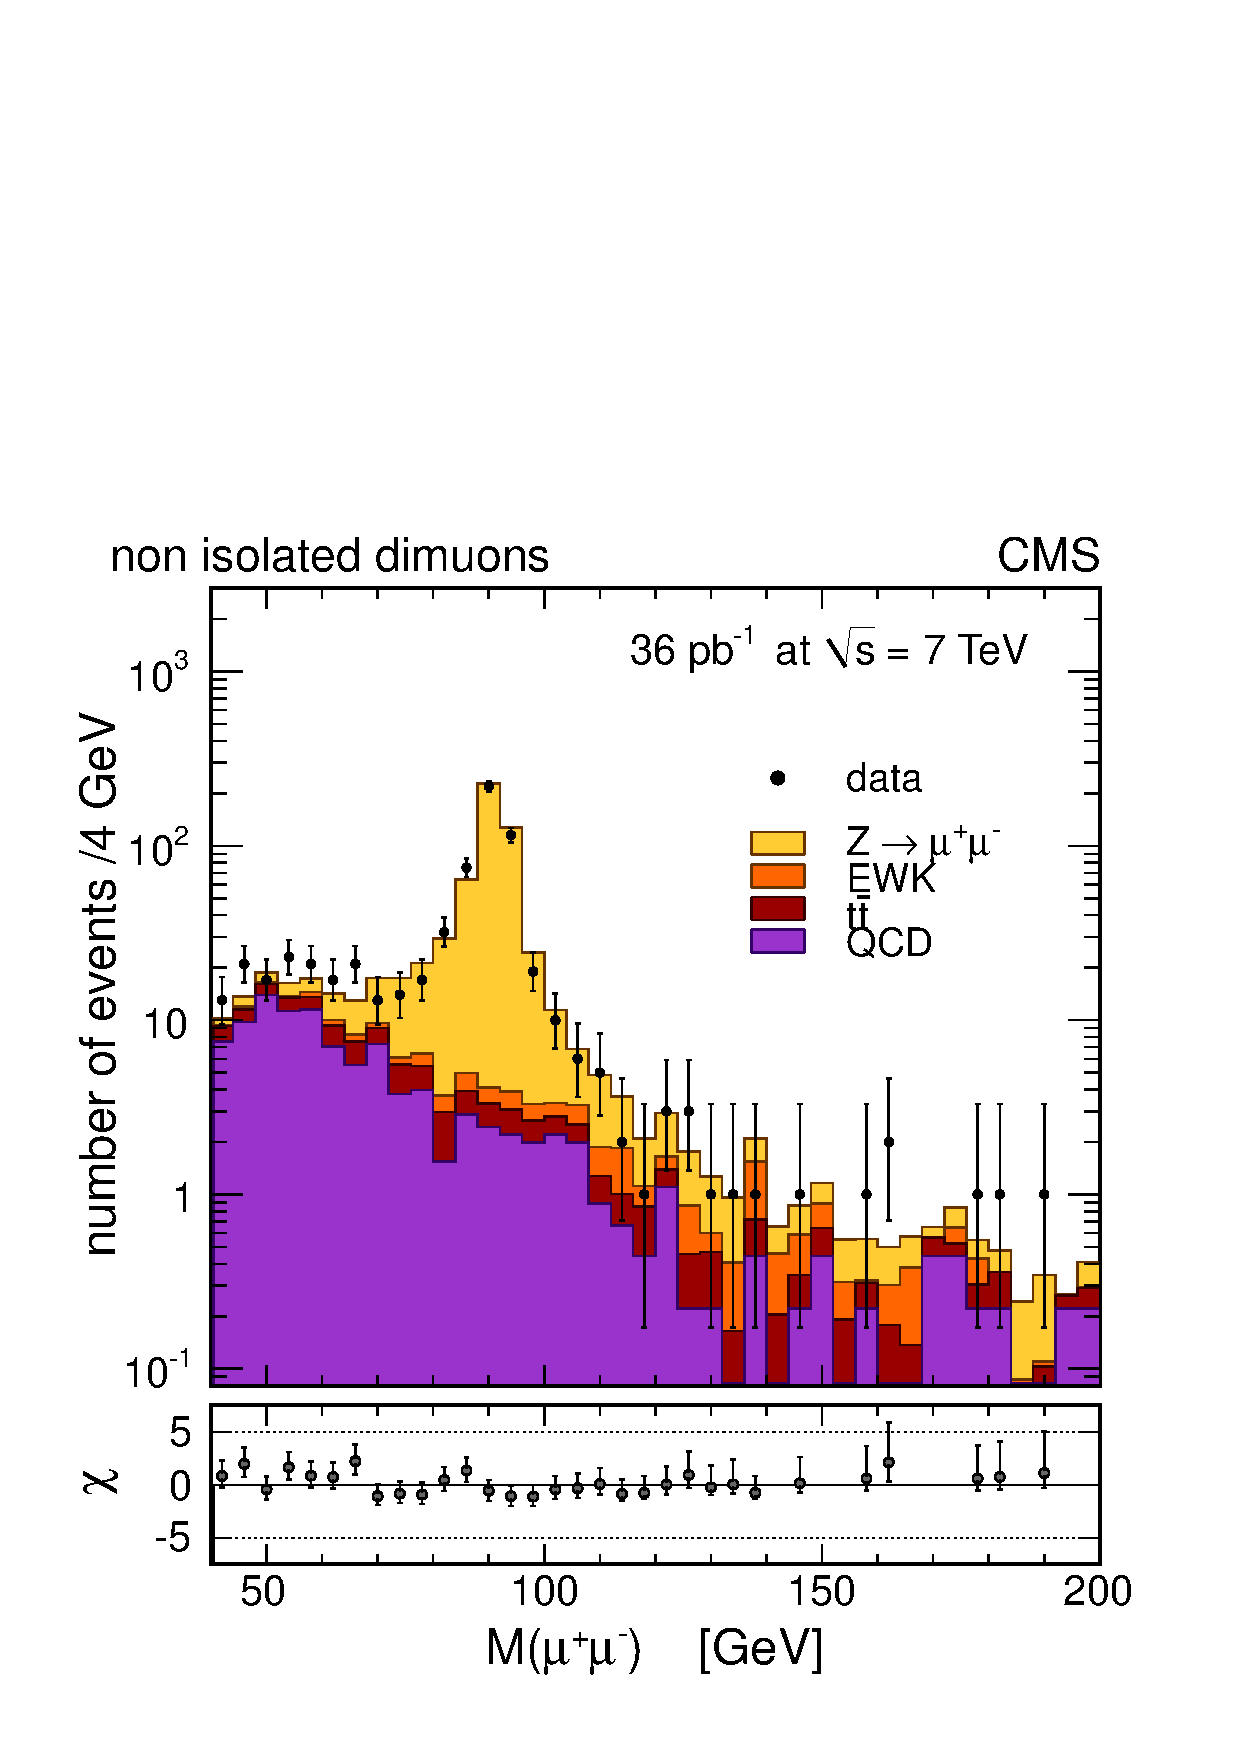
\includegraphics{figs/ZNotIso_log.pdf}}
       \end{center}
     \end{minipage}
   \end{center}
\caption{Distributions of the dimuon invariant mass for the selected
$\ZmumuNonIso$ candidates.
The points with the error bars represent the data.
Superimposed are the expected distributions from simulations, normalized
to an integrated luminosity of $36$~pb$^{-1}$. The expected distributions are
the Z signal (yellow, light histogram), other EWK processes (orange, medium histogram),
$\ttbar$ background (red, dark histogram), and QCD background (violet, black histogram).
}
\label{fig:zNoGold2}
\end{figure}

%, and the background can be considered
%negligible in the 'golden' categories (of the order of few per mille).
% \begin{eqnarray}
%    \NmumuTwoHlt (m) & = & \NmumuTwoHlt f_{peak}(m)\,, \\
%    \NmumuOneHlt (m) & = & \NmumuOneHlt f_{peak}(m)\,, \\
%    \Nmus (m) & = & \Nmus f^s_{peak}(m) + b_{\mu s}(m)\,, \\
%    \Nmut (m) & = & \Nmut f_{peak}(m) + b_{\mu t}(m)\,, \\
%    \NmumuNonIso (m) & = & \NmumuNonIso f_{peak}(m) + b_{\mu\mu}^{\mathrm{non\,iso}}(m)\,. \\
% \end{eqnarray}
The signal-peak distribution can be considered to be identical in the categories
$\Zmumu$ and $\Zmut$  because the momentum resolution in CMS is determined predominantly
by the tracker measurement for muons with $\Pt \leq 200$ GeV.
The binned spectrum of the dimuon invariant mass in the
$\Zmumu$ category, which has the most events of all categories,
is taken as shape model for all categories but $\Zmus$.
The large size of the golden sample ensures that the statistical
uncertainty of the invariant mass distribution has a negligible effect on the cross
section measurement.
The small presence of background is neglected in this distribution.
The uncertainty due to this approximation has been evaluated and
taken as the systematic uncertainty as described in Section~\ref{sec:muonSyst}.

Because only tracker isolation is used, the shape obtained from golden events
can also be used to model the $\ZmumuNonIso$ peak distribution.
A requirement on calorimetric isolation would have distorted the dimuon invariant mass
distribution of events with one nonisolated muon because of FSR,
as has been observed both in simulation and data.

The model of the invariant mass shape for the $\Zmus$ category is also derived from golden dimuon events.
The three-momentum for one of the two muons is taken from only the muon detector track fit,
in order to emulate a stand-alone muon.
To avoid using the same event twice in forming the $\Zmus$ shape model,
the higher-$\Pt$ (lower-$\Pt$) muon is chosen for even (odd) event numbers.

Background shapes are modeled as products of an exponential times a polynomial
whose degree depends on the category.
% :
% \begin{eqnarray}
%   b_{\mu t}(m) & = & N^b_{\mu t} (1 + a_1 m + a_2 m^2) e^{-\alpha m} \\
%   b_{\mu\mu}^{\mathrm{non\,iso}}(m) & = &
%   N_{\mu\mu}^{b\,\,{\mathrm{non\,iso}}} (1 + b_1 m + b_2 m^2) e^{-\beta m} \\
%   b_{\mu s}(m) & = & N^b_{\mu s} (1 + c_1 m + c_2 m^2) e^{-\gamma m}
% \end{eqnarray}
Different background models and different binning sizes are considered for the
categories other than $\Zmumu$ and a systematic uncertainty related to the fitting
procedure is determined accordingly.

%  f_{peak}^{s}(m) & = & \frac{1}{\sqrt{2\pi\sigma_s^2}} e^{-\frac{(m - M)^2}{2 \sigma_s^2} } \\
%The peak function for the $\Zmus$ category, $f_{peak}^{s}(m)$, is modeled as a
%Gaussian, due to the poor resolution, and the low statistics in that sample:

A simultaneous binned fit based on a Poissonian likelihood~\cite{PoisLR} is performed
for the different categories.
%We define, for each category, minus two times the negative logarithmic
%of the following Poissonian likelihood ratio~\cite{PoisLR}:
% \begin{equation}
% \chi^2_{\lambda} = -2 \ln{\lambda(m)} =  -2 \ln{\frac{\mathrm{Poiss}(n_i,
%     \nu_i)}{\mathrm{Poiss}(n_i, n_i)}} = \sum_{i=1}^{n_{\mathrm{bins}}} \nu_i - n_{i} + n_i \log{\frac{n_i}{\nu_i}}\,,
% \end{equation}
% where $\nu_i$ is the expected number of events in the $i^{\mathrm{th}}$-bin in $m$,
% $n_i$ is the measured number of events in that
% bin, and $\mathrm{Poiss}(n,\nu)$ is a Poissonian distribution.
% The simultaneous fit is performed minimizing the sum $R$ of the five $\chi^2_\lambda,j$ from
% the different categories $j=1,\cdots, 5$, i.e.:
% \begin{equation}
% R =  \sum_{j=1}^{5} \chi^2_{\lambda,j}   = 2  \sum_{j=1}^{5} \sum_{i=1}^{n_{\mathrm{bins}}^{(j)}} \nu^{(j)}_i - n^{(j)}_{i} + n^{(j)}_i \log{\frac{n^{(j)}_i}{\nu^{(j)}_i}}\,.
% \label{eq:PoisLR}
% \end{equation}
% For sufficiently large $\nu_i$, as in our case, the minimum of $R$ follows with good approximation a $\chi^2$ distribution,
% allowing a goodness-of-fit test.
% Using only the number of events for the two categories with the largest statistics,
% $\ZmumuTwoHlt$ and $\ZmumuOneHlt$, the Z yield and the four efficiencies can be obtained minimizing the
% following expression, which can be obtained from Eq.~\ref{eq:PoisLR} using a single bin in the Gaussian approximation for $\ZmumuTwoHlt$
% and $\ZmumuOneHlt$:
% \begin{eqnarray*} \label{chi2}
% R & = &
% \frac{(\NmumuTwoHlt - \NZtomumu\effHlt^2\effIso^2\effTrk^2\effSa^2)^2}{\NmumuTwoHlt} +  \\
% & & \frac{(\NmumuOneHlt - 2\NZtomumu\effHlt(1-\effHlt)\effIso^2\effTrk^2\effSa^2)^2}{\NmumuOneHlt} +  \\
% & & \chi^2_{\lambda, \mu s} +
% \chi^2_{\lambda, \mu t} +
% \chi^{\nonIso\,\, 2}_{\lambda, \mumu}\, ,
% \end{eqnarray*}
% where we use the event counts only in the  $\ZmumuOneHlt$ and $\ZmumuTwoHlt$ 'golden'
% categories and the Poissonial terms $\chi^2_{\lambda, \mu s}$, $\chi^2_{\lambda, \mu t}$ and
% $\chi^{\nonIso\,\, 2}_{\lambda, , \mumu}$ for the remaining categories.
% The likelihood ratio fit is equivalent to an ordinary $\chi^2$
% for sufficiently large statistics and we verified that, with the current data sample,
% it gives the same central value and statistical uncertainty.
%We perform the fit in the range $60 < m < 120~\mathrm{GeV}/c^2$.
%Full details on the signal and background modeling assumptions and
%correlation studies are present in~\cite{CMS_AN_2010-345}.
Table~\ref{fig:fitRes_36pb} reports the signal yield and single-muon efficiencies determined from
the simultaneous fit and the ratios of the fitted to simulation efficiencies.
A goodness-of-fit test gives a probability ($p$-value) of 0.36 for this fit.

%The resulting fit $p$-value shows the good quality of the fit.
%With the analyzed statistics, a second degree polynomial function is
%taken for modeling  the background shape.

\begin{table}[htbp] %L.L.
\begin{center}
\caption{Signal yield and efficiencies determined from data with the simultaneous fit, and
  ratios of efficiencies determined from the fit and the simulation.}
\label{fig:fitRes_36pb}
\begin{tabular}{|c|c|c|}
\hline
Quantity & Fit results from data & Data/simulation\\
\hline\hline
$\NZtomumu$ &13\,728 $\pm$ 121   & \\
\hline
$\effHlt$ & 0.9203 $\pm$ 0.0019  &0.9672 $\pm$ 0.0020   \\
$\effIso$ & 0.9813 $\pm$ 0.0010& 0.9962 $\pm$  0.0011 \\
$\effSa$ & 0.9762  $\pm$ 0.0012 & 0.9964 $\pm$ 0.0013 \\
$\effTrk$ & 0.9890 $\pm$ 0.0006  & 0.9949 $\pm$ 0.0007  \\
\hline
\end{tabular}
\end{center}
\end{table}

%In order to correct the fitted yield $\NZtomumu$ for the presence of background,
%the estimated irreducible background fraction is subtracted.
%$f_{bkg}=0.44 \pm 0.02\%$.

The background in the $\Zmumu$ golden category (of the order of few per mille)
was neglected in the fit. In order to correct the fitted yield $\NZtomumu$ for
the presence of this background, we subtract the small estimated irreducible
background fraction.

A $(1.0\pm 0.5)\%$ overall efficiency correction due to the loss of muon events because of trigger
prefiring is also applied (Section~\ref{sec:muonEff}).

The estimated cross section is $968\pm 8 \mathrm{(stat.)}$~pb.

As cross-check, a simpler analysis based on event counting was also performed.
The same selection was applied, and the number of events with two global muon, reported
in Sec~\ref{sec:muonid}, was used as signal yield. 
The signal yield was then corrected for the relevant efficiencies that have 
been evaluated with a \TNP method in a single $\Pt$ and $\eta$ bin, resulting in a
cross section estimate of $969\pm 8 \mathrm{(stat.)}$~pb, in good agreement
with the simultaneous fit method.

